\newcommand{\ClassPath}{../../../yukibook.cls}
\documentclass{\ClassPath/yukibook}


\begin{document}

    \yukibook{Planificación y administración de redes} % Title
    {Rubén Gómez}  % Author
    {2021-2022}    % Year
    {Técnico superior en Administración de \linebreak Sistemas informáticos en red} % Name of degree
    {}% catch phrase
    {}% the phrase's author
    {img/portada.png} %cover
    {28436c}
    {sgbd} %mini-title

    \coverpage
    \licensepage

    \tableofcontents

    %--------------------------------------------------------------------------
    % Start your parts, chapters and sections here
    %--------------------------------------------------------------------------
    \part{Planificación y administración de redes}
    \graphicspath{{img/redes/}}
    \chapter{Introducción a los sistemas de comunicación}

\section{Introducción}

Desde el principio de los tiempos, el ser humano se ha comunicado con sus congéneres de distintas maneras: comenzó a través de la voz (se cree que hace unos 100.000 años), con algún tipo de protolenguaje, para posteriormente comenzar a utilizar sistemas de comunicaciones permanentes (la escritura).

Por todos es conocido la evolución histórica de distintos sistemas escritos, entre los que podemos destacar (\href{https://es.wikipedia.org/wiki/Anexo:Cronolog%C3%ADa_de_las_tecnolog%C3%ADas_de_la_comunicaci%C3%B3n}{referencia}):
\begin{itemize}
    \item \textbf{Pinturas rupestres}: Realizadas en cuevas o rocas en las que se pueden observar escenas de caza, distintos animales, grabado de manos, figuras humanas... Algunas de las pinturas encontradas cuentan con más de 50.000 años. Tenemos un ejemplo cercano en las \href{https://es.wikipedia.org/wiki/Cueva_de_Santimami\%C3\%B1e}{cuevas de Santimamiñe} en donde tenemos pinturas datadas entre 14.000 y 9.000 años a. C.

    \item \textbf{Escritura cuneiforme}: Es uno de los primeros sistemas de escritura realizados, y se utilizaban tablillas de arcilla húmeda en las que se grababa mediante un tallo vegetal. Con este sistema se han datado tablas anteriores al 3.200 a.C. y en distintos idiomas.

    \item \textbf{Escritura jeroglífica y el papiro}: En el antiguo Egipto se crea la escritura mediante signos que comienza por escribirse en paredes para posteriormente inventar el papiro (cuya datación más antigua es del 2.500 a.C.) y de esta manera se comienza a tener un sistema de comunicación fácilmente manejable e intercambiable.

    \item \textbf{Uso de palomas mensajeras}: El uso de palomas mensajeras para el envío de comunicaciones data de la época anterior a 1.500 a.C. y se ha estado utilizando hasta este siglo en algunos países durante desastres naturales.

    \item \textbf{Telégrafo}: A partir de mediados del siglo XVIII y durante el inicio del siglo XIX hubo bastantes avances en las investigaciones del electromagnetismo y de esta manera se comenzó a investigar cómo usarlo para el envío de señales. En 1837 Samuel Morse patenta el \href{https://es.wikipedia.org/wiki/Tel%C3%A9grafo#Historia_del_tel%C3%A9grafo}{telégrafo}. En \textbf{1858} se une Irlanda y Terranova mediante el \textbf{primer cable trasatlántico}.

    \item \textbf{Teléfono}: Como evolución al telégrafo, que sólo permitía el envío de señales, nace el teléfono de la mano de \href{https://es.wikipedia.org/wiki/Antonio_Meucci}{Antonio Meucci} (aunque normalmente se le atribuye el invento a \href{https://es.wikipedia.org/wiki/Alexander_Graham_Bell}{Alexander Graham Bell}). En 1860 realizó una demostración pública transmitiendo voz a una considerable distancia.
\end{itemize}

Tal como podemos ver, ha habido distintos sistemas de comunicación utilizados durante siglos para el envío y recepción de información.

\section{Comunicación de la información}

Tal como hemos visto, los sistemas de comunicación de la información no es algo nuevo, ¿pero qué necesidades tiene un sistema de comunicación?

\begin{itemize}
    \item \textbf{Emisor}: Es el origen y la fuente de la información que se pretende comunicar.
    \item \textbf{Receptor}: Es el destinatario, el que va a recibir la información.
    \item \textbf{Mensaje}: Es la información que queremos transmitir entre el emisor y el recepetor.
    \item \textbf{Código}: Es el conjunto de reglas utilizadas a la hora de representar el mensaje. El emisor y receptor deben utilizar el mismo código para que la comnunicación sea correcta.
    \item \textbf{Canal}: Es el medio físico por el que se va a enviar el mensaje.
    \item \textbf{Señal}: Es el componente físico por el que se envía la información.
\end{itemize}

Para entender de mejor manera un sistema de comunicación y los componentes que lo forman, vamos a poner dos ejemplos:

\subsubsection*{Ejemplo 1: Comunicación oral}

\begin{wrapfigure}{r}{0.25\linewidth}
    \centering
    \vspace{-35pt}
    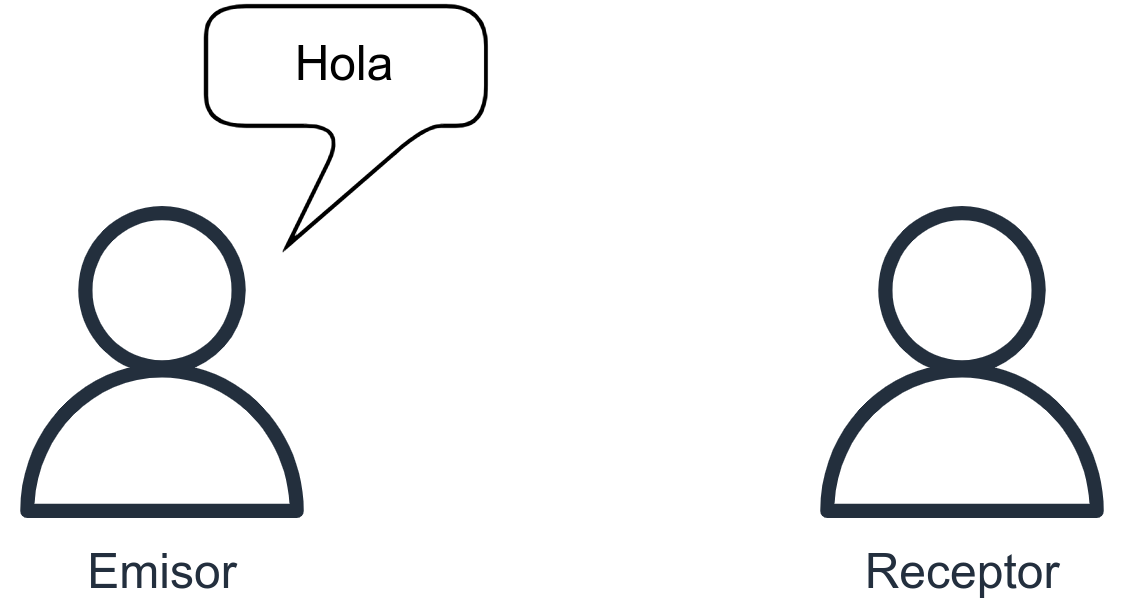
\includegraphics[width=\linewidth]{comunicacion-1.png}
    \vspace{-30pt}
\end{wrapfigure}
En este ejemplo vemos que hay dos personas, las cuales se han identificado cada una de ellas como “Emisor” y “Receptor”, y así de esta manera conocemos quién es el origen y quién el destino de la comunicación.

En este caso, el \textbf{mensaje} es “Hola”, haciendo uso del \textbf{código} conocido como “castellano”. La \textbf{señal} que se va a utilizar es la voz, ya que están hablando y el \textbf{canal} por el que se envía el mensaje es el aire.

Es un ejemplo sencillo que utilizamos cada día.

\subsubsection*{Ejemplo 2: Comunicación escrita por mensajería}

\begin{wrapfigure}{r}{0.25\linewidth}
    \centering
    \vspace{-35pt}
    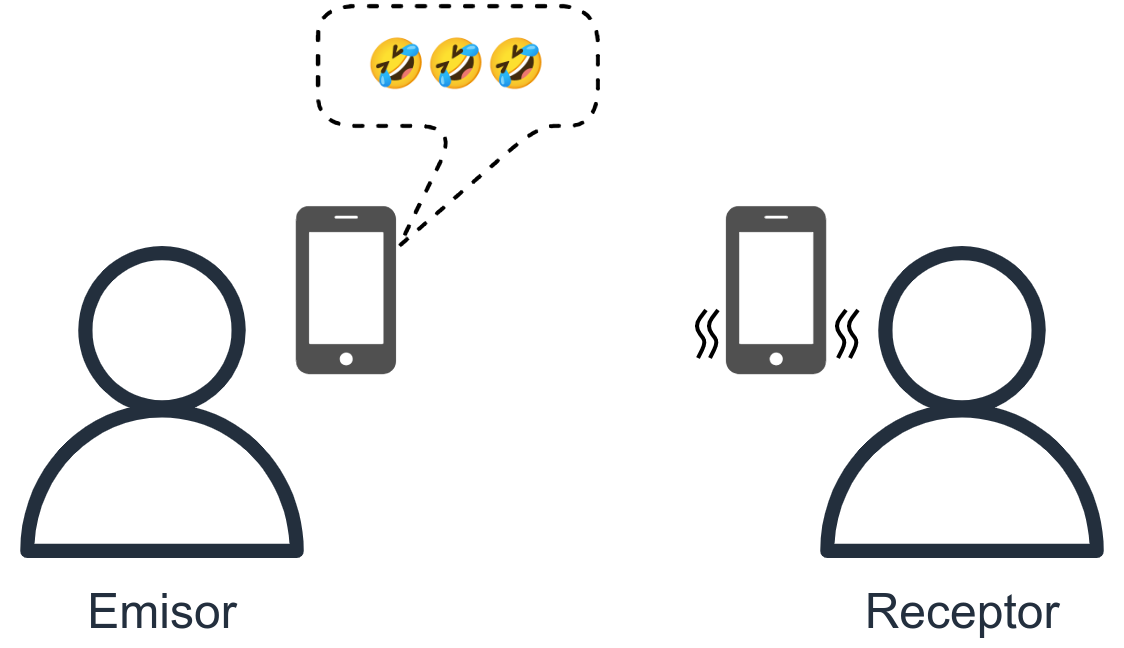
\includegraphics[width=\linewidth]{comunicacion-2.png}
    \vspace{-30pt}
\end{wrapfigure}
AL igual que en el ejemplo anterior, vemos que hay dos personas, las cuales se han identificado cada una de ellas como “Emisor” y “Receptor” pero que en este caso se van a comunicar haciendo uso de un teléfono móvil, tal como hacemos en nuestro día a día a través de una aplicación de mensajería o red social.

Teniendo en cuenta esto, en este ejemplo realmente existen dos sistemas de comunicación que están mezclados y uno está por encima del otro:

\begin{itemize}
    \item \textbf{Entre personas}: Similar al ejemplo anterior, el emisor y el receptor se están comunicando, con el mensaje compuesto por tres \href{https://es.wikipedia.org/wiki/Emoji}{emojis} que representan estar riendo. El \textbf{código} es el idioma que estén utilizando, el \textbf{canal} sería el programa utilizado y la \textbf{señal} podríamos decir que es el móvil.

    \item \textbf{Entre dispositivos}: En este caso, el emisor y receptor es el móvil de cada usuario. El mensaje es el mismo, pero convertido a un sistema digital (como el \hyperlink{binario}{binario}). El \textbf{canal} en este caso sería el aire y la \textbf{señal} es la utilizada por el móvil, por ejemplo el 5G.
\end{itemize}

Tal como se puede ver en este caso, una comunicación puede depender a su vez de otro sistema de comunicación.

\subsection{Esquema de la comunicación}
Para simplificar cómo se realiza la comunicación, podemos utilizar el siguiente esquema:

\begin{center}
    \vspace{-10pt}
    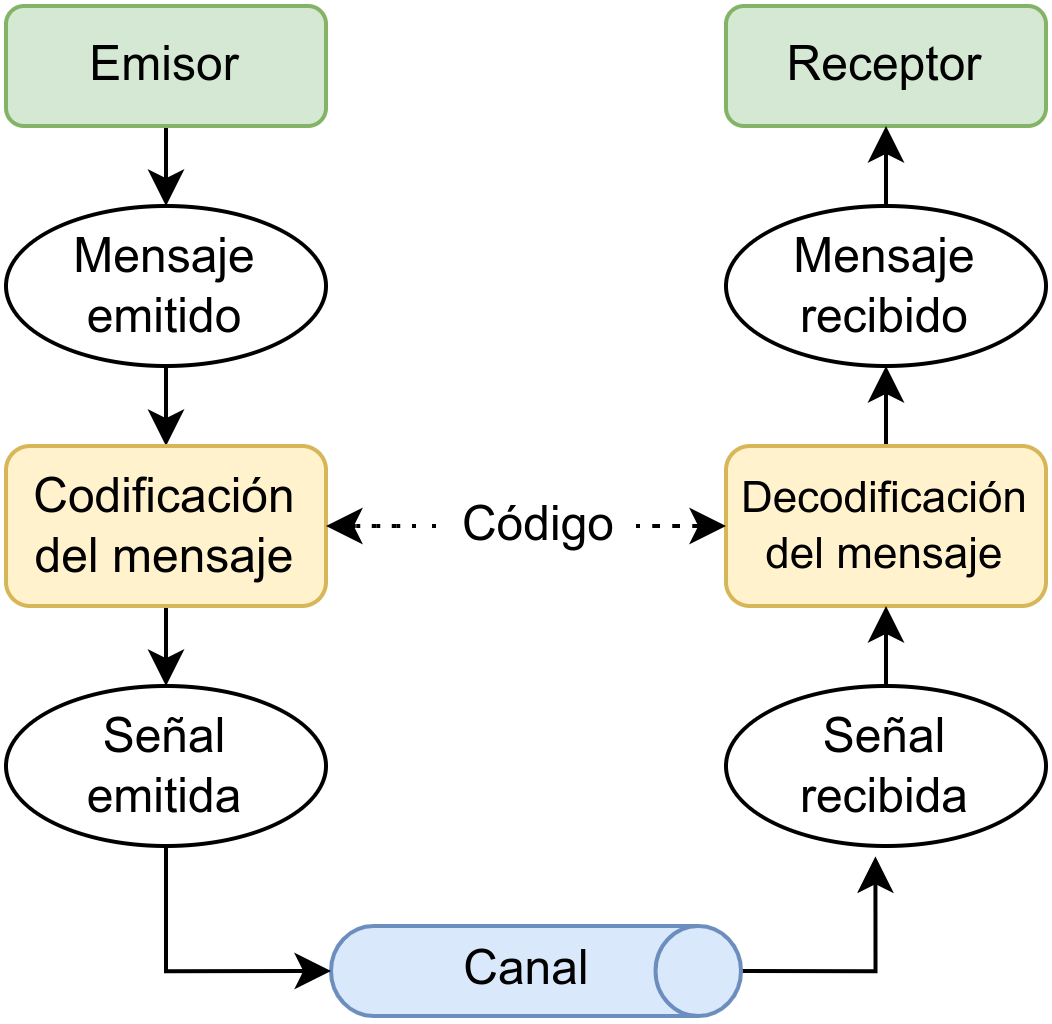
\includegraphics[width=0.6\linewidth]{comunicacion-esquema.png}
    \vspace{-10pt}
\end{center}


\section{Sistemas de numeración}
La información que queremos retransmitir debe estar representada de alguna manera, y tal como hemos visto previamente, \textbf{a través de un código que tanto emisor como receptor deben conocer}.

En sistemas orales, o escritos, lo habitual es hacer uso de un idioma concreto mediante un alfabeto conocido. En informática se hace uso de distintos sistemas de numeración para representar tanto números como el resto de información.

\subsection{Sistema decimal}
El ser humano, desde hace tiempo ha utilizado como sistema para contar el sistema decimal, representado mediante el sistema \href{https://es.wikipedia.org/wiki/N%C3%BAmeros_ar%C3%A1bigos}{arábigo}. Posiblemente se adoptó este sistema por contar con 10 dedos en las manos.

El sistema numérico decimal está basado en diez símbolos ordenados (0, 1, 2, 3, 4, 5, 6, 7, 8, 9), situados de manera ponderada (cada posición tiene un peso específico), que permiten representar las cantidades deseadas. Debido a que hacemos uso de diez símbolos se dice que utiliza la \textbf{base 10}.

\subsubsection*{Representación}
Cuando se combina con otros sistemas de numeración, debemos indicar la base en la forma $ \mathbf{19_{(10}} $ , es decir, poniendo un pequeño “\textbf{(10}” a la derecha del número representado la base 10.

La representación de cualquier combinación del sistema decimal se puede representar en forma de potencia, donde la base es 10 (como ya hemos visto antes) y el exponente es la posición en la que se sitúa el símbolo.

Vamos a tomar como ejemplo el siguiente número: \textbf{146}. La representación en forma de potencias:

\begin{center}
    \vspace{-10pt}
    $ 146 =1\times10^2 + 4\times10^1 + 6\times10^0 $

    $ 146 = 1\times100 + 4\times10 + 6\times1 $

    $ 146 = 100+40+6 $
\end{center}

Como se puede comprobar, lo que hemos hecho ha sido coger cada símbolo representado y lo hemos multiplicado por la base (en este caso base 10) y a la base le hemos puesto el exponente de la posición en la que se encuentra. \textbf{El símbolo de más a la derecha tiene como exponente el cero}, y hacia la izquierda el exponente se incrementa en uno para cada posición.


\hypertarget{binario}{}
\subsection{Sistema binario}

En informática el sistema binario es el más importante ya que es el sistema que internamente utilizan los circuitos digitales. En este sistema sólo se hace uso de dos símbolos, el “0” y el “1”, y por tanto \textbf{su base es 2}. Los dos dígitos se denominan \textbf{bits} (contracción de \textbf{binary digit}).

\subsubsection*{Representación}

Para representar que estamos haciendo uso del sistema binario debemos indicar la base al lado del número, por ejemplo: $\mathbf{ 101001_{(2}} $. Como se puede ver es añadir “\textbf{(2}” en pequeño al final del último símbolo.


\subsection{Sistema hexadecimal}

Esta vez necesitamos dieciséis símbolos ordenados, así que es un sistema de \textbf{base 16}. Para la representación se hace uso de los símbolos numéricos que conocemos (0, 1, 2, 3, 4, 5, 6, 7, 8, 9) y para representar los siguientes, las letras “A”, “B”, “C”, “D”, “E” y “F”, de esta manera formamos los 16 símbolos que necesitamos.

Teniendo en cuenta esto, podemos hacer la representación directa de que $\mathbf{A_{(16} = 10_{(10}}$ y que $\mathbf{E_{(16} = 14_{(10}}$.

En informática es muy habitual hacer uso del sistema hexadecimal a la hora de trabajar con \textbf{bytes} (que es una “palabra” de \textbf{8 bits}). Un símbolo hexadecimal se representa como 4 bits, por lo que necesitaríamos 2 símbolos hexadecimales para un byte.

También se usa durante la edición de código en formato de datos, o durante la programación en ensamblador.

\subsubsection*{Representación}
Al igual que con los sistemas anteriores, debemos añadir la base cuando estemos utilizando el sistema hexadecimal: $\mathbf{ F17A_{(16}} $ , $\mathbf{ FBE1D_{(16}} $ , $\mathbf{ 1FAB27_{(16}} $


\subsection{Sistema octal}
En ordenadores antiguos era habitual hacer uso del sistema octal. Hoy día se usa más como sistema intermedio entre binario y hexadecimal.

Esta vez nos basamos en ocho símbolos ordenados (0, 1, 2, 3, 4, 5, 6, 7), que, al combinarlos, permiten representar las cantidades deseadas. Debido a que hacemos uso de ocho símbolos se dice que utiliza la \textbf{base 8}.

\subsubsection*{Representación}
Para representar la base, debemos añadir “(8” a la derecha del número que hayamos indicado, como por ejemplo: $\mathbf{ 770_{(8} }$ , $\mathbf{ 175_{(8}} $


\subsection{Conversiones entre los distintos sistemas de numeración}

Hasta ahora no nos habíamos encontrado con distintos sistemas de numeración, pero ahora que conocemos cuatro de ellos, tenemos que saber que existe la posibilidad de realizar conversiones entre ellos.


Una vez entendidos los distintos sistemas de numeración nos tiene que quedar claro que aunque la representación de los símbolos sea la misma, el número o cantidad representada no es la misma. Por ejemplo:

\errorbox{
    \begin{center}
        $\mathbf{ 1010_{(10}  \neq  1010_{(2}  \neq  1010_{(16}  \neq 1010_{(8}} $
    \end{center}
}

A continuación se va a explicar cómo realizar conversiones entre los distintos sistemas de numeración que hemos visto, y a modo de resumen está la \hyperlink{tabla_conversiones_directas}{tabla de conversiones directa}.

\subsubsection{Conversión de decimal a...}
La manera más sencilla para realizar las distintas conversiones partiendo de un número decimal es hacer divisiones sucesivas usando la base a la que queremos realizar la conversión.

\subsubsection*{... binario}
Se trata de dividir sucesivamente el número decimal y los sucesivos cocientes entre dos (la base binaria).

Vamos a utilizar como ejemplo el número decimal $\mathbf{27_{(10}}$ :

\begin{center}
    \vspace{-20pt}
    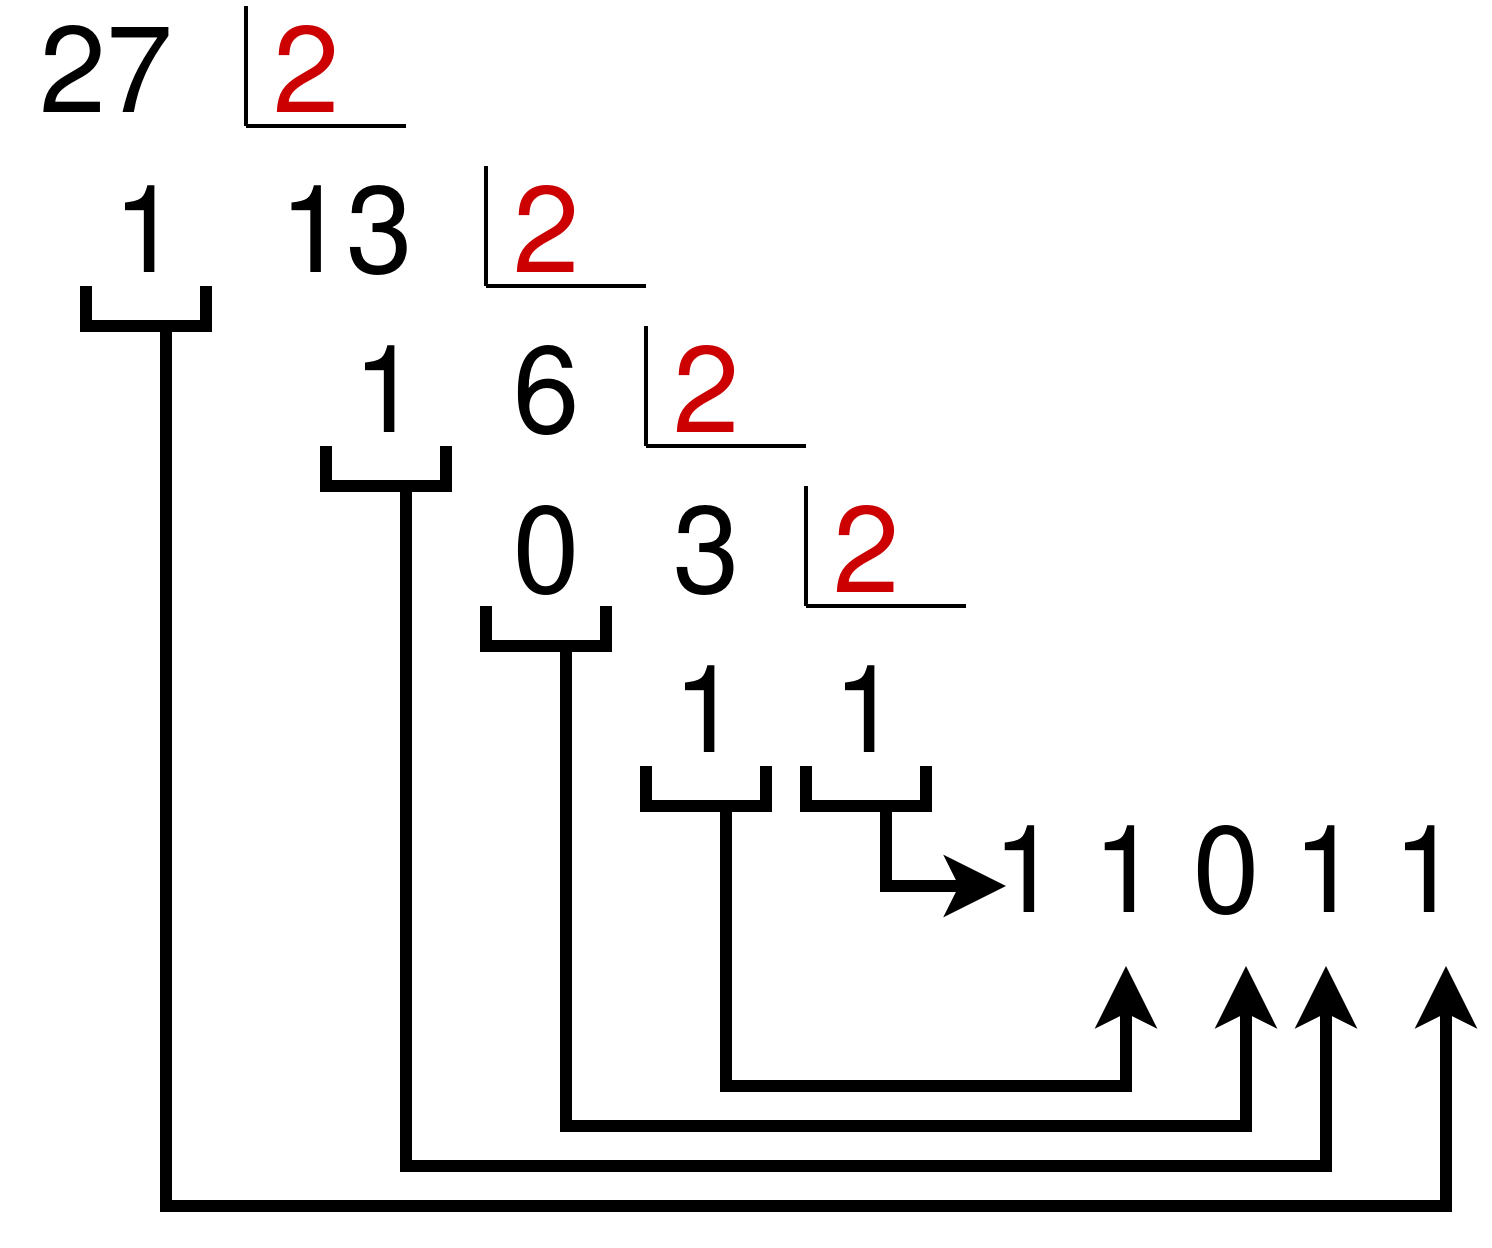
\includegraphics[width=0.29\linewidth]{decimal_binario.png}
    \vspace{-20pt}
\end{center}

\textbf{Los restos los cogemos en orden inverso} para obtener la siguiente equivalencia: $\mathbf{27_{(10} = 11011_{(2}}$

\subsubsection*{... hexadecimal}
Se trata de dividir sucesivamente el número decimal y los sucesivos cocientes entre 16 (la base hexadecimal). Cuando el cociente o resto sea entre 10 y 15, habrá que cambiarlo por la letra correspondiente.

\begin{center}
    \vspace{-10pt}
    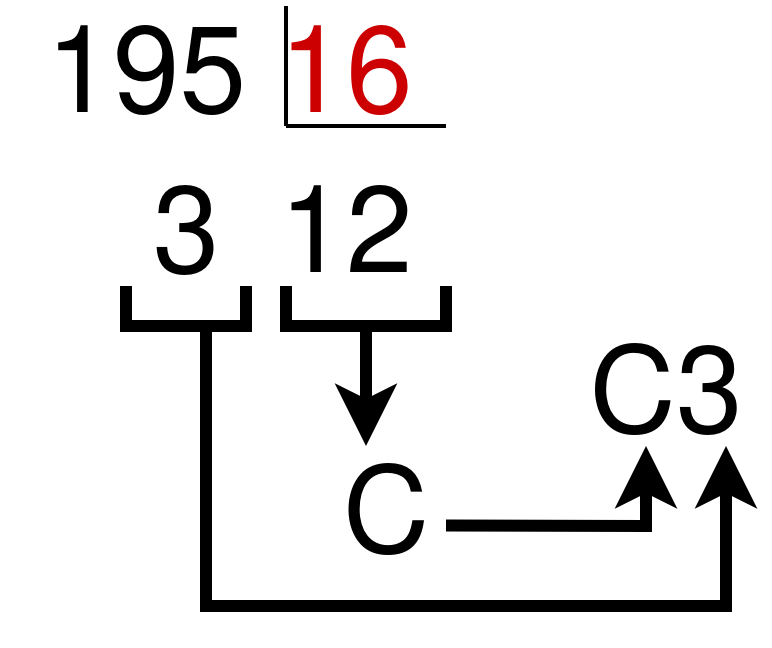
\includegraphics[width=0.2\linewidth]{decimal_hexadecimal.png}
    \vspace{-15pt}
\end{center}

\textbf{Los restos los cogemos en orden inverso} para obtener la siguiente equivalencia: $\mathbf{195_{(10} = C3_{(16}}$

\subsubsection*{... octal}
Al igual que los anteriores, hacemos divisiones sucesivas:

\begin{center}
    \vspace{-10pt}
    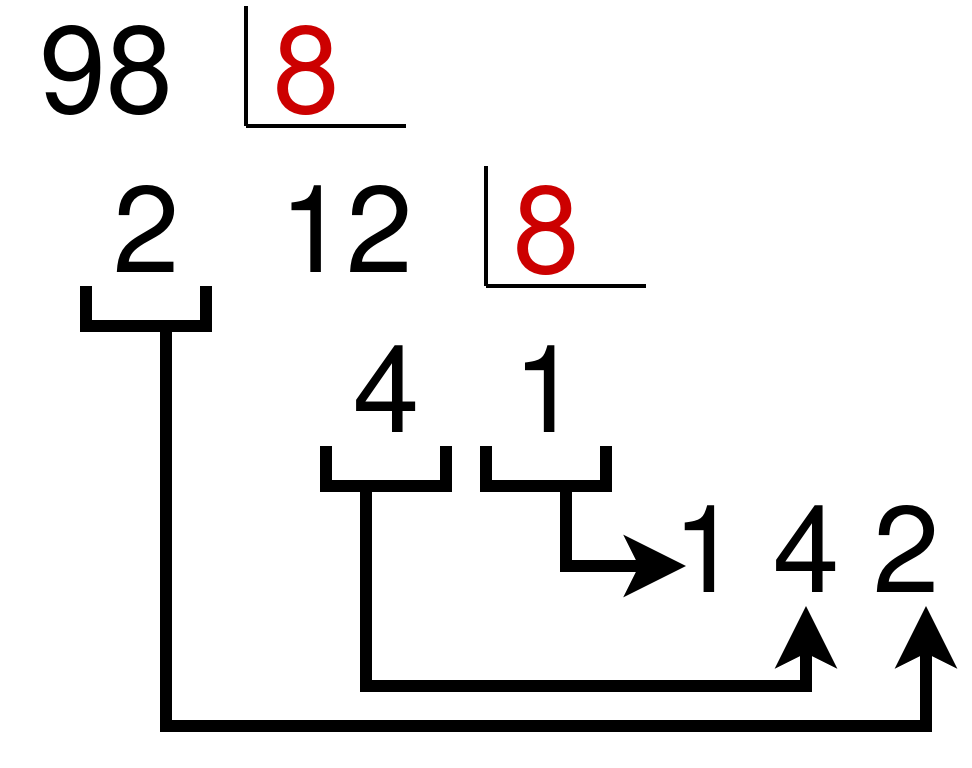
\includegraphics[width=0.25\linewidth]{decimal_octal.png}
    \vspace{-15pt}
\end{center}

\textbf{Los restos los cogemos en orden inverso} para obtener la siguiente equivalencia: $\mathbf{98_{(10} = 142_{(8}}$


\subsubsection{Conversión de binario a...}

\subsubsection*{... decimal}
El sistema de numeración binario es un sistema posicional donde cada dígito binario (bit) tiene un valor basado en su posición relativa al \textbf{LSB} (\textit{Least Significant Bit} = bit menos significativo, que es el que está más a la derecha y que tiene el menor valor).

Cualquier número binario puede convertirse a su equivalente decimal multiplicando cada bit por la base (2) y usando como exponente la posición (siendo 0 el exponente del bit de más a la derecha). Para ilustrarlo, cojamos como ejemplo el número binario $\mathbf{11011_{(2}}$:

\begin{center}
    \vspace{-20pt}

    $ \mathbf{11011_{(2}} $

    $ \mathbf{1\times2^4 + 1\times2^3 + 0\times2^2 + 1\times2^1 + 1\times2^0} $

    $ \mathbf{16 + 8 + 0 + 2 + 1 = 27_{(10}} $
    \vspace{-15pt}
\end{center}

Nótese que el procedimiento consiste en determinar los valores (es decir, las potencias de 2) de cada posición de bit que contenga un 1 y luego sumarlos.

Nótese también que el \textbf{MSB} (\textit{Most Significant Bit} = bit más significativo, el que está más a la izquierda, el que tiene mayor valor) tiene un valor de $\mathbf{2^4}$ a pesar de que es el quinto bit. Esto se debe a que el \textbf{LSB} (\textit{Least Significant Bit}, el bit menos significativo, el que está a la derecha) es el primer bit y tiene un valor de $\mathbf{2^0}$.

\subsubsection*{... octal}
Para convertir un número binario a octal \textbf{se agrupan los dígitos de 3 en 3 empezando desde el lado derecho} hacia la izquierda, sustituyendo cada trío de dígitos binarios por su equivalente en octal.

Si en el lado izquierdo quedase algún bit “suelto” (sin formar un grupo de 3), se pueden poner “0” a la izquierda.

Cogemos como ejemplo el número binario $\mathbf{1100101001001_{(2}}$ para pasarlo a octal, haremos:

\begin{center}
    \vspace{-15pt}
    $\mathbf{001\ \ 100\ \ 101\ \ 001\ \ 001_{(2} = 14511_{(8}}$
    \vspace{-15pt}
\end{center}

\subsubsection*{... hexadecimal}
Similar al caso anterior, pero en este caso \textbf{la agrupación que se realiza debe de ser de 4 en 4 bits}. Si usamos el mismo ejemplo anterior $\mathbf{1100101001001_{(2}}$ :

\begin{center}
    \vspace{-15pt}
    $\mathbf{0001\ \ 1001\ \ 0100\ \ 1001_{(2} = 1949_{(16}}$
    \vspace{25pt}
\end{center}



\subsubsection{Conversión de hexadecimal a...}
\subsubsection*{... binario}
Para pasar de hexadecimal a binario convertiremos cada símbolo hexadecimal a 4 dígitos binarios.

\begin{center}
    \vspace{-15pt}
    $\mathbf{F17A_{(16} = 1111\ \ 0001\ \ 0111\ \ 1010_{(2}}$

    $\mathbf{1A4F_{(16} = 0001\ \ 1010\ \ 0100\ \ 111_{(2}}$
    \vspace{-15pt}
\end{center}


\subsubsection*{... decimal}
Al igual que hemos hecho con las conversiones previas a decimal, se podría realizar haciendo potencias de 16, pero se entiende que es más complicado de realizar.

Por lo tanto, \textbf{la manera más sencilla es pasar primero a binario} como acabamos de ver \textbf{y posteriormente convertir ese binario a decimal} como hemos visto previamente.

\subsubsection*{... octal}
Pasar primero a binario y después a octal.



\subsubsection{Conversión de octal a...}
\subsubsection*{... binario}
Cada dígito en octal se convierte en su representación en 3 bits:

\begin{center}
    \vspace{-15pt}
    $\mathbf{167_{(8} = 001\ \ 110\ \ 111_{(2}}$

    $\mathbf{253_{(8} = 010\ \ 101\ \ 011_{(2}}$
    \vspace{-15pt}
\end{center}
Los ceros de la izquierda se podrían quitar, ya que no alteran el valor.

\subsubsection*{... decimal}
Se puede realizar de dos maneras. La primera es hacer uso de potencias de 8 (similar al paso de pasar de binario a decimal, pero cambiando la base):

\begin{center}
    \vspace{-15pt}
    $\mathbf{157_{(8} = 1\times8^2 + 5\times8^1 + 7\times8^0 = }$

    $\mathbf{1\times64 + 5\times8 + 7\times1 = }$

    $\mathbf{64 + 40 + 7 = 111_{(10}}$

    Resultado: $\mathbf{157_{(8} = 111_{(10}}$
    \vspace{-15pt}
\end{center}

Con números grandes puede ser un poco complicado calcular las potencias de 8, por lo que \textbf{la alternativa es pasarlo primero a binario} como hemos visto, \textbf{y después pasarlo de binario a decimal}.

\subsubsection*{... hexadecimal}
La manera más sencilla es realizar la conversión primero a binario tal como hemos visto, y posteriormente pasar el número binario a hexadecimal como se ha visto previamente.


\chapter{Redes de comunicación}
En el ámbito informático una red de comunicaciones es representada como una red de ordenadores. Las redes de ordenadores son un conjunto de equipos hardware que están conectados entre sí (ya sea mediante cables o de manera inalámbrica) y que a través de un software especializado envían y reciben impulsos eléctricos (u ondas electromagnética) para el transporte de datos. De esta manera podrán compartir información, recursos u ofrecer servicios.


\section{Breve historia de las redes}
A continuación una breve cronología mostrando los hitos más importantes dentro de las redes de comunicaciones, en lo que a ordenadores se refiere (\href{https://en.wikipedia.org/wiki/Computer_network}{Referencia}).

\begin{description}
    \item[\textasciitilde 1950]
    En la década de los 50 se desarrollan los circuitos integrados. Esto hará que en el futuro los ordenadores cada vez se vayan haciendo más pequeños.

    Las redes de ordenadores comienzan a aparecer en las bases militares americanas, en principio para sistemas de radares.

    \item[\char`\~ 1960]
    Se realiza una conexión entre dos mainframes en EEUU para el sistema de reservas aéreas comerciales.

    El \href{https://es.wikipedia.org/wiki/Instituto_de_Tecnolog%C3%ADa_de_Massachusetts}{MIT} utiliza un ordenador para enrutar y mantener conexiones telefónicas.

    En 1966, aparece un paper (artículo científico) describiendo las WAN.

    En 1969 ARPANET (red de ordenadores creadas por el Departamento de Defensa de Estados Unidos) cuenta con 4 nodos (a 50kbit/s de velocidad).

    \item[\char`\~ 1970]
    En 1972 se hace la primera demostración pública de ARPANET.

    A comienzos de la década (1973) se crea Ethernet en la compañía Xerox Parc.

    A finales de la década Xerox intenta hacer que Ethernet se convierta en un estándar de conexión para terminar con las competencias (token ring, …).

    \begin{center}
        \vspace{-10pt}
        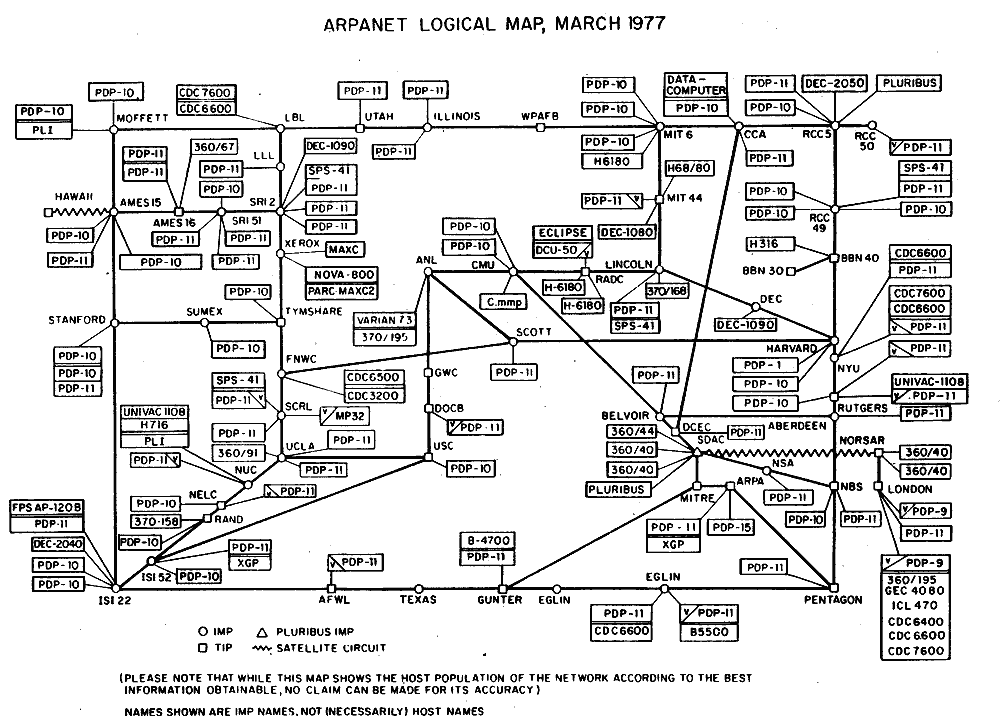
\includegraphics[frame,width=0.9\linewidth]{Arpanet_logical_map_march_1977.png}
        \vspace{-5pt}
        \captionof{figure}{Mapa lógico de ARPANET, marzo de 1977. Origen: \href{https://es.wikipedia.org/wiki/ARPANET\#/media/Archivo:Arpanet_logical_map,_march_1977.png}{ Wikipedia}}\vspace{-13pt}
    \end{center}

    \item[\char`\~ 1980]
    Los ordenadores personales empiezan a generalizarse.

    Aparece el protocolo para enviar y recibir e-mails (SMTP).

    El protocolo TCP/IP se convierte en el utilizado por ARPANET (1983) y es declarado como su estándar para las comunicaciones.

    Aparece el servicio DNS.

    Se crea el modelo de referencia OSI.

    Aparece el primer gusano por la red (Morris worm, 1988). Se estima que infectó al 10\% de los ordenadores conectados a la red.

    Se crea el protocolo BGP.

    El protocolo Ethernet evoluciona y permite conexiones a 10Mbit/s.


    \item[\char`\~ 1990]
    Tim Berners-Lee desarrolla el código para WWW y crea el primer servidor web (1991).

    Se puede decir que aquí es cuando nace la Internet que conocemos actualmente.

    En 1995 Ethernet permite conexiones a 100Mbit/s

    Se establece un control para los nombres de dominio (posteriormente lo asumirá ICANN).

    Aparece Amazon, ebay, Craiglist, IMDB, hotmail, google, yahoo, ...

    Aparece el protocolo IPv6 (1998).

    Aparece el protocolo wifi 802.11b.

    \item[\char`\~ 2000]
    Crisis de las “.com”.

    Internet se generaliza.

    Empiezan a permitirse más TLDs, que no corresponden sólo a países.

    Ethernet permite conexiones a 1Gbit/s

    \item[\char`\~ 2010]
    Ethernet permite conexiones a 400Gbit/s (2018).

    \href{https://en.wikipedia.org/wiki/Starlink}{Starlink} comienza a desplegar su constelación de satélites para dar cobertura en todo el planeta.


\end{description}

\section{Tipos de redes}
A la hora de diferenciar las redes de ordenadores podemos diferenciarlas por distintos conceptos:

\begin{itemize}
    \item Por el medio de transmisión utilizado.
    \item Por la dirección de los datos.
    \item Por el alcance.
    \item Por el grado de acceso.
    \item Por la topología.
    \item ...
\end{itemize}

\subsection{Por el medio de transmisión utilizado}
Más adelante veremos distintos \hyperlink{sistemas_transmision}{sistemas de transmisión}, pero para ir diferenciando podemos crear dos grandes grupos teniendo en cuenta el medio utilizado:

\begin{itemize}
    \item \textbf{Guiados}: Es decir, a través de cables que se encargarn de realizar la transmisión de la señal desde un punto de origen al punto de destino.

    \item \textbf{No guiados}: Se hace uso de algún sistema inalámbrico (mediante antenas) para realizar la transmisión de los datos.
\end{itemize}


\subsection{Por la dirección de los datos}
Si tenemos en cuenta la dirección de los datos en la transmisión, podemos diferenciarlos como:

\begin{itemize}
    \item \textbf{Simplex}: la comunicación sólo se realiza en un único sentido, por lo que sólo es necesario un único canal de transmisión.

    \item \textbf{Half-duplex}: se permite la comunicación en ambos sentidos, pero no de manera simultánea, por lo que emisor y receptor se reparten el tiempo de emisión. Por ejemplo, el \textit{\textbf{walkie-talkie}}.

    \item \textbf{Duplex}: O también conocido como \textit{full-duplex}, permite la comunicación en ambas direcciones y de manera simultánea. Por ejemplo, el \textbf{teléfono}. Para ello es necesario tener una de estas dos opciones:
    \begin{itemize}
        \item Dos canales Half-duplex: uno para cada dirección de la comunicación.
        \item Un único canal por el que se envía la comunicación, pero para ello es necesario algún sistema de multiplexación (como puede ser usar frecuencias separadas).
    \end{itemize}
\end{itemize}


\subsection{Por alcance}
Teniendo en cuenta el alcance al que llegan las redes, podríamos realizar la siguiente distinción:

\subsubsection{Red de área personal (PAN)}
Del inglés \textit{Personal Area Network}, es aquella en la que interactúan distintos dispositivos de muy corto alcance, limitado al área de una persona.

El ejemplo más habitual hoy día sería la comunicación mediante tecnología inalámbrica por Bluetooth en la comunicación entre ordenador, móvil y dispositivos como un \textit{smartwatch}.


\subsubsection{Red de área local (LAN)}
Del inglés \textit{Local Area Network}, es una red que puede abarcar un cierto área de tamaño como una casa, una oficina, un colegio, una universidad...

El ejemplo de una oficina sería una red en la que existen distintos ordenadores, que pueden comunicarse entre sí o compartir información con un servidor ya sea a través de una red cableada o también inalámbrica.

\subsubsection{Red de área metropolitana (MAN)}
Del inglés \textit{Metropolitan Area Network}, y como su nombre indica, el área es mayor y suele abarcar una ciudad para ofrecer los servicios necesarios en la misma.

En este caso también puede ser de manera cableada (normalmente haciendo uso de tecnología más rápida como es la fibra óptica) y también de manera inalámbrica.

Dentro de los servicios que pertenecerían a una MAN podemos poner como ejemplos:
\begin{itemize}
    \item Despliegue de zonas WIFI gratuito en la ciudad.
    \item Comunicación entre sistemas de información (paradas de autobuses, marquesinas, ...).
    \item Sistemas de video-vigilancia municipal.
\end{itemize}

Algunos de estos servicios que están en una MAN pueden ser públicos (como el WIFI) o de acceso restringido (sistemas de seguridad).

\subsubsection{Red de área amplia (WAN)}
Del inglés \textit{Wide Area Network}, es una red que abarca grandes extensiones geográficas y normalmente construidas por grandes empresas o proveedores de internet (ISP, \textit{Internet Service Provider}).


\subsection{Por el grado de acceso}
Teniendo en cuenta quién puede acceder a la red, podríamos definir dos tipos de redes:

\begin{itemize}
    \item \textbf{Red privada}: es una red que sólo ciertas personas pueden acceder y que no normalmente no es accesible desde otras redes. El ejemplo más sencillo es la red que tenemos en casa.
    \item \textbf{Red pública}: es una red a la que puede acceder cualquier persona y que interconecta otras redes sin importar su situación geográfica. Internet es una red pública.
\end{itemize}

\subsection{Por la topología}
La topología de una red indica cómo están interconectados los nodos de la misma y el camino que pueden realizar los datos cuando viajan por esa red. En resumen: \textbf{es el diseño de la red}.

%TODO: completar información






\chapter{Arquitectura en capas}
Un sistema de comunicación se pueden diferenciar en distintos niveles en los que cada uno realiza una función independiente, pero que a su vez interactúan con los niveles limítrofes.

\begin{center}
    \vspace{-10pt}
    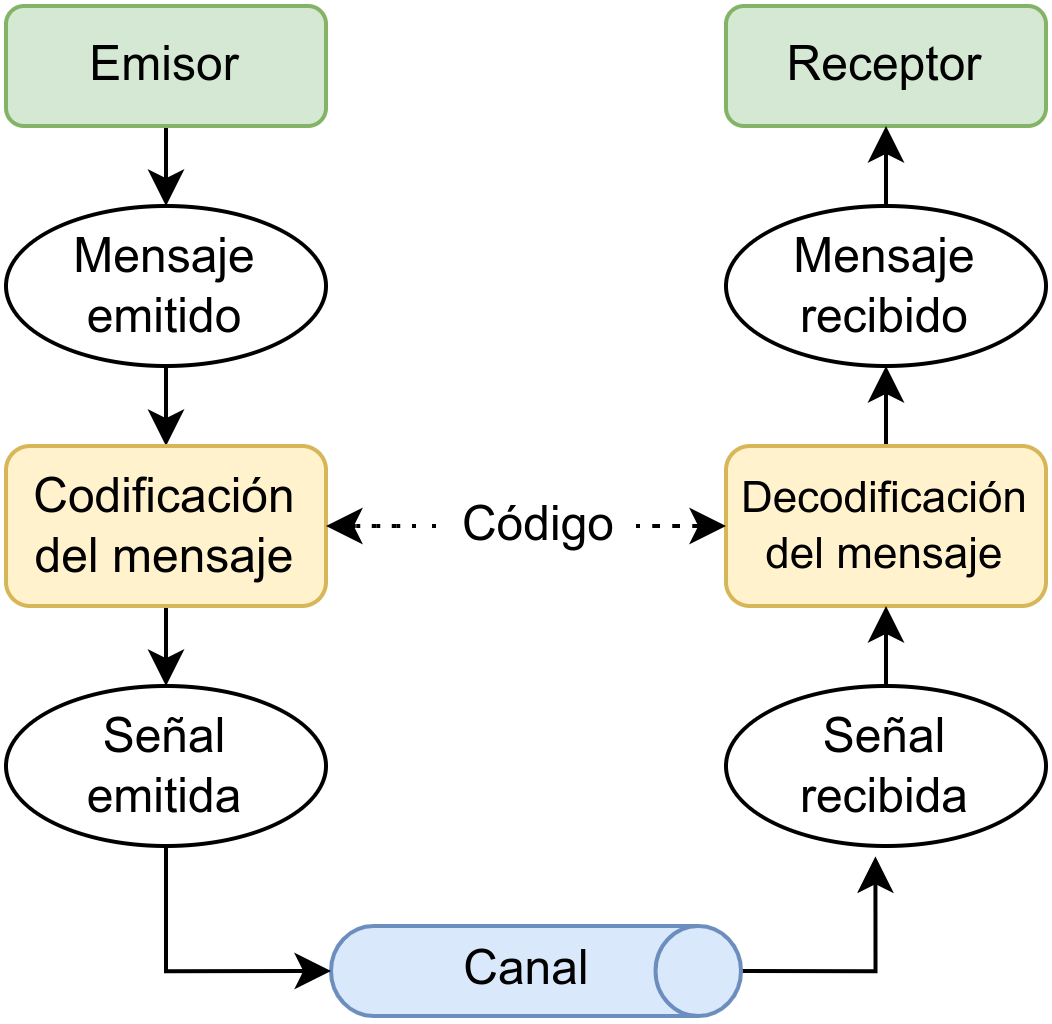
\includegraphics[width=0.4\linewidth]{comunicacion-esquema.png}
    \vspace{-10pt}
\end{center}

Este ejemplo es un modelo simplificado de comunicación, y dentro de una arquitectura de red de ordenadores pueden existir más capas en las que pueden existir distintas funciones extra que no aparecen en este esquema.

\section{Origen}

Al comienzo de las redes de ordenadores cada empresa creaba su propio sistema de comunicación creando su propio hardware y software, lo que hacía imposible la interconexión entre equipamiento de distintas empresas.

Estos sistemas de comunicación constan de unas reglas que los nodos deben conocer para poder comunicarse entre sí, y a ese conjunto de reglas se les denomina \textbf{protocolo de comunicación}.


Para que eso hoy en día no suceda ya que las redes están definidas en varios estándares, como veremos más adelante.

\infobox{Un \textbf{estándar} es un conjunto de normas que pueden abarcar distintos niveles (tanto software como hardware) que ha sido aceptado, o creado, por la gran mayoría de las empresas del sector para poder realizar la interconexión e intercomunicación entre sí.}


\section{Ventajas de la división en capas}

La división en capas nos permite:
\begin{itemize}
    \item Dividir el proceso de comunicación en procesos más pequeños.

    \item Aislar las funciones de cada capa. De esta manera, en caso de realizar modificaciones en la misma, no afecta al resto de capas.

    \item Ocultar la implementación al resto de capas. Siguiendo con el punto anterior, una capa utilizará los servicios de su capa inferior sin saber cómo realiza sus funciones.

    \item Cada capa puede constar de distintos estándares, facilitando la interconexión de distintas tecnologías
\end{itemize}

Una arquitectura de red en capas se implementa por medio de distintos protocolos, formando una familia de protocolos para facilitar la comunicación de distintos sistemas y equipos en la red.

\infobox{Una arquitectura en capas nos permite que cada capa actúe de manera independiente y que incluya sus propios protocolos. Cada capa dispone de una serie de servicios que ofrece a su capa limítrofe superior.}

Desde el comienzo de las redes de ordenadores han existido distintas familias de protocolos, y se puede considerar que hubo una \href{https://en.wikipedia.org/wiki/Protocol_Wars}{guerra de protocolos durante las décadas de 1970 a 1990}. Empresas, organizaciones y países se posicionaban sobre cuál sería el mejor protocolo de comunicaciones y el que saldría ganador para el uso a nivel internacional.

Por destacar algunos protocolos que ya no se usan:

\begin{itemize}
    \item \textbf{\href{https://en.wikipedia.org/wiki/Systems_Network_Architecture}{SNA}} creado en 1974 por IBM.
    \item \textbf{\href{https://en.wikipedia.org/wiki/NetBIOS_Frames}{NetBEUI}} de Microsoft. Que evolucionó a NetBIOS sobre TCP/IP que hoy día se usa en Windows Server.
    \item \textbf{\href{https://en.wikipedia.org/wiki/IPX/SPX}{IPX/SPX}} de Novell.
\end{itemize}

\section{Modelo de referencia OSI}
El modelo de interconexión de sistemas abiertos, conocido como “modelo \textbf{OSI}” (\textit{\textbf{O}pen \textbf{S}ystems \textbf{I}nterconnection} en inglés) es un \textbf{modelo de referencia (teórico)} que busca estandarizar las funciones de comunicación para un sistema informático siendo agnóstico a la tecnología utilizada para realizar la implementación y a los protocolos utilizados en cada capa.

El diseño comenzó en 1977 tratando de terminar con la \href{https://en.wikipedia.org/wiki/Protocol_Wars}{guerra de protocolos} comentada previamente, y la Organización Internacional de Estandarización (\textit{International Organization for Standardization}, o \textbf{ISO} en inglés)  terminó por definir el estándar ISO-7498 en 1984.


\subsection{Capas en el modelo OSI}
El modelo OSI está compuesto por siete capas numeradas del 1 al 7 siendo la 1 la más baja y haciendo referencia a la parte física de la red.


\begin{table}[H]
    \centering
    \tablestyle
    \begin{tabular}{|L{0.15\linewidth}|L{0.3\linewidth}|L{0.46\linewidth}|}
        \theadstart
        \thead \textbf{Capa} &
        \thead \textbf{Nombre de la unidad de datos} &
        \thead \textbf{Función} \tabularnewline
        \tbody
        7ª - Aplicación & Datos
            & APIs de alto nivel, como compartir recursos y acceso remoto a archivos.
            \\ \hline
        6ª - Presentación & Datos
            & Traducción de datos entre un servicio de red y una aplicación, que incluye la codificación de caracteres, la compresión de datos y el cifrado y descifrado de datos.
            \\ \hline

        5ª - Sesión & Datos
            & Manejo de sesiones de comunicación, por ejemplo el continuo intercambio de información en forma de múltiples transmisiones hacia ambos lados entre dos nodos.
            \\ \hline

        4ª - Transporte & Segmento, Datagrama
            & Transmisión de segmentos de datos confiable entre puntos de red, incluyendo la segmentación, el acknowledgement y la multiplexación.
            \\ \hline

        3ª - Red & Paquete
            & Estructura y manejo de una red multinodo. Incluye el direccionamiento, el ruteo y el control de tráfico traffic control.
            \\ \hline

        2ª - Enlace & Trama
            & Transmisión de datos confiable entre dos nodos conectados mediante una capa física.
            \\ \hline

        1ª - Física & Bit, Baudios
            & Transmisión y recepción de flujos de bits sin procesar por un medio físico.
            \\ \hline

        \tend
    \end{tabular}
    \vspace{-10pt}
\end{table}






\section{Arquitectura TCP/IP}





\chapter{Conexión de redes a nivel físico}



\hypertarget{sistemas_transmision}{}
\section{Sistemas de transmisión}

guiados:
- cable par trenzado
- coaxial
- optica
FTTH

no guiados
- radiofrecuencia



\chapter{Conexión de redes a nivel de enlace de datos}


\section{Administración de switches}



\chapter{Interconexión de redes}
Hoy en día no suele ser habitual tener redes completamente aisladas, ya que la comunicación sólo se podría realizar entre los nodos y los dispositivos de la misma.

En el momento en el que una red quiera comunicarse con otra vamos a necesitar de un dispositivo que realice de intermediación para el intercambio de paquetes, y ese dispositivo es el \textbf{router}.

\section{Router}

\begin{wrapfigure}{r}{0.36\linewidth}
    \centering
    \vspace{-20pt}
    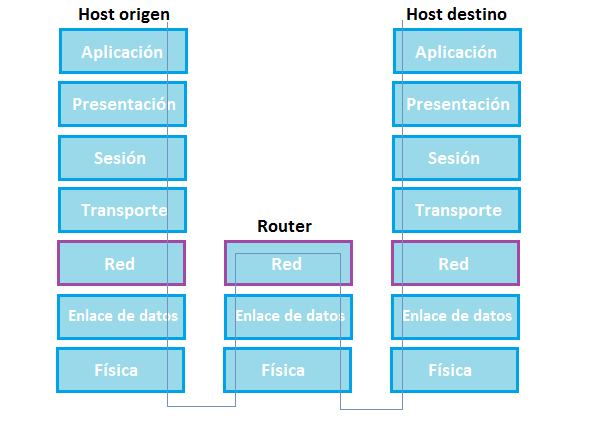
\includegraphics[width=\linewidth]{OSI_model_router.png}
    \vspace{-32pt}
    \captionof{figure}{Router en el modelo OSI (\href{https://es.wikipedia.org/wiki/Router\#/media/Archivo:OSI_model_router.png}{wikipedia})}
    \vspace{-10pt}
\end{wrapfigure}

Un router (o encaminador) es el encargado de enrutar (o encaminar) los paquetes que recibe de una red a otra red buscando la ruta más adecuada para ello.

Un router puede “unir” redes, por lo que para ello es necesario que tenga interfaces configuradas (IPs) en las redes que quiere comunicar. Tendrá tantas interfaces configuradas como redes a las que esté unido.


\begin{center}
    \vspace{-15pt}
    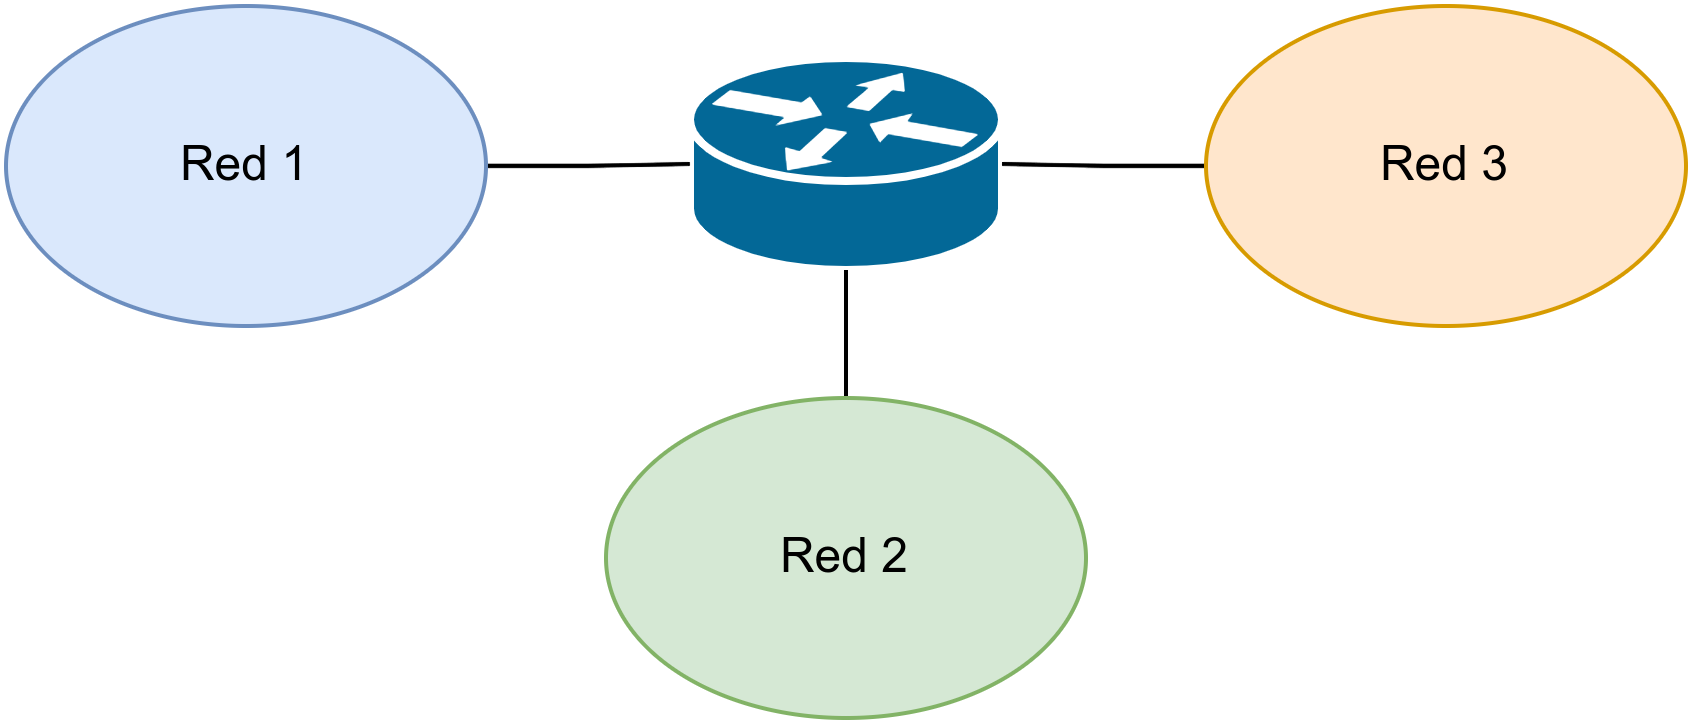
\includegraphics[width=0.6\linewidth]{router_redes.png}
    \vspace{-5pt}
    \captionof{figure}{Router conectado a 3 redes}
    \vspace{-15pt}
\end{center}

El ejemplo más sencillo de router lo tenemos en casa, que es proporcionado por nuestro ISP. Este router une la red privada donde conectamos nuestros equipos (PCs, tablets, móviles) y la red del proveedor que a su vez nos dará acceso a Internet.


\subsection{Puerta de enlace predeterminada}
La puerta de enlace predeterminada (en inglés \textit{\textbf{default gateway}}) es el dispositivo por defecto por el que irá la comunicación de un equipo cuando trate de comunicarse con una red que no es la suya.

Sin una puerta de enlace, nuestro PC sólo podría comunicarse con otros equipos de la misma red, ya que el switch se encarga de ello, pero no podríamos realizar ninguna comunicación con ningún equipo que estuviese fuera de la red.

\warnbox{\textbf{Los routers también pueden tener puertas de enlace predeterminadas.}}

Los gateway también tienen otras funciones a la hora de intercomunicar redes, como por ejemplo:
\begin{itemize}
    \item Traducir la información que se envía utilizando el protocolo de la red de origen al protocolo utilizado en la red de destino.
    \item Realizar enmascaramiento de la IP de la red origen cambiándola por la IP del dispositivo en la red de destino (también conocido como \hyperlink{nat}{NAT}).
\end{itemize}

Un equipo sólo podrá contar con una puerta de enlace predeterminada configurada, pero mediante \hyperlink{rutas_estaticas}{rutas estáticas} podremos elegir cómo encaminar tráfico a otras redes destino.

\infobox{\textbf{Un equipo sólo podrá contar con una puerta de enlace predeterminada configurada.}}

Para saber cuál es la puerta de enlace de un equipo informático, dependeremos del sistema operativo en el que nos encontremos. En un entorno GNU/Linux actual podremos obtenerlo por consola de la siguiente manera:

\begin{mycode}{Obtener puerta de enlace en GNU/Linux}{console}{}
ruben@ubuntu:~$ ip route
default via 192.168.1.1 dev enp1s0 proto dhcp metric 100
\end{mycode}

En distribuciones antiguas se hacía
\begin{mycode}{Obtener puerta de enlace en GNU/Linux}{console}{}
ruben@ubuntu:~$ route -n

Kernel IP routing table
Destination     Gateway      Genmask      Flags Metric Ref  Use Iface
0.0.0.0      192.168.1.1     0.0.0.0      UG    100    0    0   enp1s0
\end{mycode}


En un entorno Windows, podremos verlo a través del interfaz gráfico yendo a “\textbf{Configuración → Estado de red → Cambiar opciones del adaptador}”, donde veremos los adaptadores que tiene nuestro equipo. Seleccionaremos uno, y haciendo click derecho le daremos a “\textbf{Estado → Detalles}”

\begin{center}
    \vspace{-15pt}
    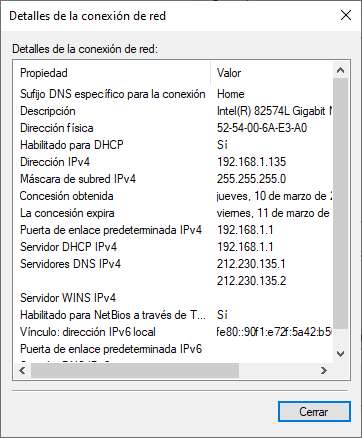
\includegraphics[frame,width=0.4\linewidth]{windows_network_status.png}
    \vspace{-15pt}
\end{center}

Para no dar tantos pasos, si ejecutamos en la terminal \textbf{CMD} el siguiente comando también lo veremos:

\begin{mycode}{Obtener puerta de enlace en Windows}{powershell}{}
C:\Users\ruben> ipconfig

Configuración IP de Windows
Adaptador de Ethernet Instancia de Ethernet 0 2:

Sufijo DNS específico para la conexión. . : Home
Vínculo: dirección IPv6 local. . . : fe80::90f1:e72f:5a42:b50d%7
Dirección IPv4. . . . . . . . . . . . . . : 192.168.1.135
Máscara de subred . . . . . . . . . . . . : 255.255.255.0
Puerta de enlace predeterminada . . . . . : 192.168.1.1
\end{mycode}

Pueden existir equipos sin puerta de enlace, pero no suele ser lo habitual. Esto sucede cuando queremos que equipos puedan ver a otros equipos de la red, pero no puedan comunicarse con el exterior. Suele ser más habitual realizar bloqueos a nivel de firewall.


\hypertarget{nat}{}
\section{NAT}
La traducción de direcciones de red, también llamado enmascaramiento de IP o NAT (del inglés \textit{\textbf{Network Address Translation}}), es un mecanismo utilizado por routers que conectan dos (o más) redes para que el paquete que llega a un equipo destino no parezca que llega desde la red de origen.

Vamos a tomar como ejemplo el siguiente esquema que es un ejemplo que podemos entender teniendo en cuenta la conexión de nuestra casa:

\begin{center}
    \vspace{-15pt}
    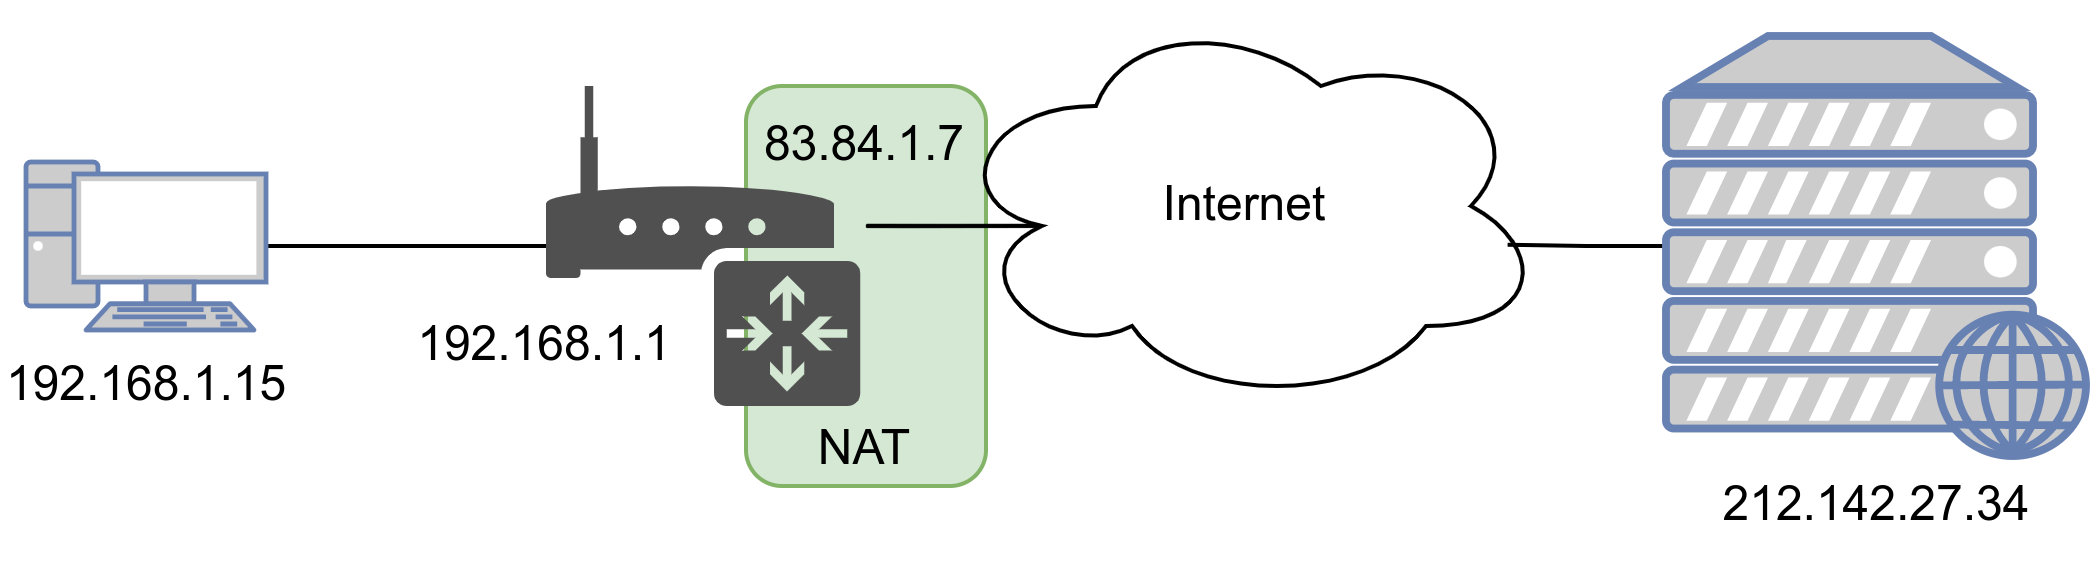
\includegraphics[width=0.8\linewidth]{NAT.png}
    \vspace{-25pt}
\end{center}

En este ejemplo tenemos conectado un equipo con IP 192.168.1.15 al router que tenemos en casa (cuya IP en la LAN es 192.168.1.1). Este router cuenta con una IP pública proporcionada por el ISP para el acceso a internet (83.84.1.7). Cuando nuestro equipo quiere comunicarse con algún equipo que no está en su red, al salir a internet, el router cambia la cabecera del paquete sustituyendo 192.168.1.15 por 83.84.1.7, y de esta manera al servidor remoto (212.142.27.34) el paquete le llega desde una IP pública.

Este es el ejemplo más sencillo y que hacemos uso cada día en casa, pero esto no significa que NAT sólo se realice entre redes públicas y privadas. Lo podemos utilizar entre dos redes públicas o dos redes privadas también.

Las traducciones de dirección se almacenan en una tabla, para recordar qué dirección y puerto le corresponde a cada dispositivo cliente y así saber donde deben regresar los paquetes de respuesta.

Existen distintos tipos de NAT:
\begin{itemize}
    \item \textbf{NAT de sobrecarga}: Varios equipos de la red de origen se traducen por una única dirección de la red de salida. Es el método más habitual (el que realizan nuestros routers en casa).

    \item \textbf{NAT estática}: También conocida como “NAT 1:1”, ya que una dirección IP privada se traduce siempre por una única dirección IP pública, y siempre será la misma. Este método es el habitual cuando queremos tener un servidor en la red interna y queremos que su comunicación con el exterior siempre sea con la misma IP pública

    \item \textbf{NAT dinámica}: Similar al caso anterior, pero en este caso el router contará con una tabla de IPs públicas y se asignará una que esté libre de esta tabla a un equipo interno cuando necesite comunicarse de manera pública. Cuando deje de necesitarlo, la IP se marcará como “libre” y se podrá asignar a otro equipo interno posteriormente.
\end{itemize}


\section{Encaminamiento de tráfico a otras redes}

Tal como hemos dicho, un router se encarga de encaminar el tráfico entre redes, ya sean redes a las que esté directamente conectado o no. En caso de que sea un paquete a una red ajena, existen distintas maneras de tratarlo:

\begin{itemize}
    \item Reenviar el tráfico a la puerta de enlace predeterminada.
    \item Consultar la tabla de enrutamiento (o tabla de rutas).
\end{itemize}

La tabla de enrutamiento se almacena en los routers y nos indicará cómo llegar a nodos u otras redes a las que no tenemos acceso de manera directa. La tabla de enrutamiento se puede genera haciendo uso de:

\begin{itemize}
    \item \textbf{Rutas estáticas}: deben ser introducidas a mano.
    \item \textbf{Rutas dinámicas}: mediante un protocolo de enrutamiento dinámico.
\end{itemize}


\hypertarget{rutas_estaticas}{}
\subsection{Rutas estáticas}
Las rutas estáticas sirven para obligar a los paquetes, cuyo destino coincide con la ruta, a ir a través de la puerta de enlace especificada, en lugar de ir por la puerta de enlace predeterminada. Lógicamente, para que esto suceda, la puerta de enlace tiene que ser alcanzable por el router, por lo que tenemos que tener acceso a través de la misma red.


La ruta estática se configura para conseguir conectividad con un dispositivo que no esté directamente conectado al equipo que tenga las rutas. Las rutas estáticas permiten la construcción manual de la tabla de enrutamiento.

\begin{center}
    \vspace{-15pt}
    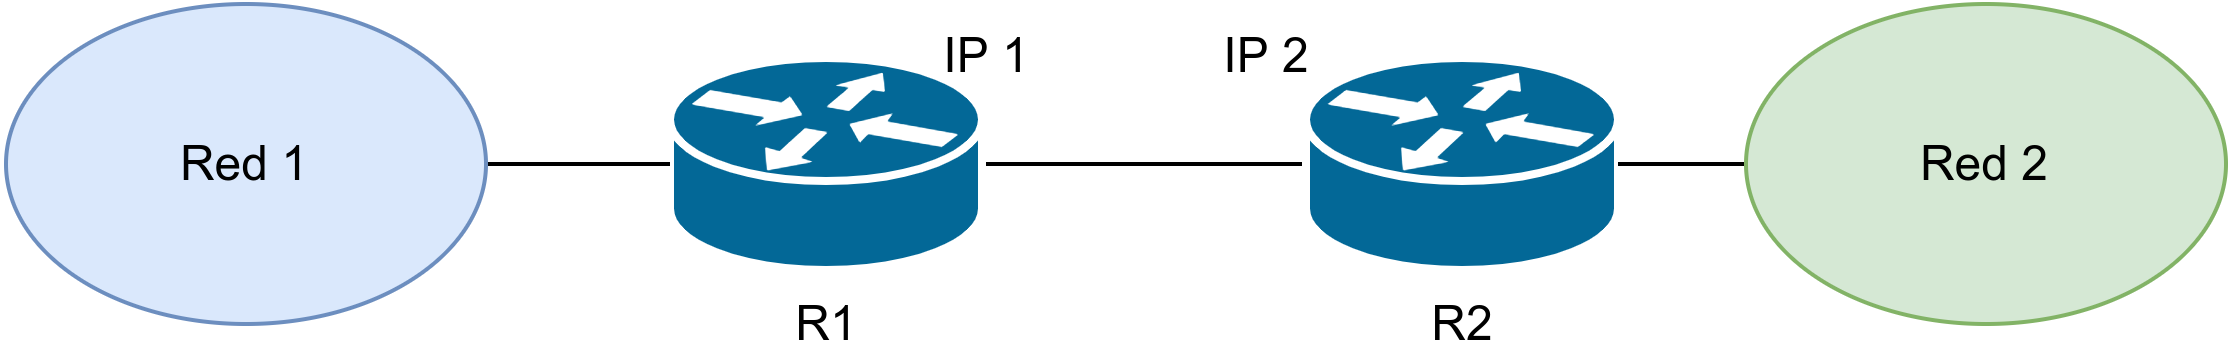
\includegraphics[width=0.8\linewidth]{rutas_estaticas.png}
    \vspace{-25pt}
\end{center}

Teniendo en cuenta el dibujo, para que un equipo de la red 1 pueda comunicarse con un equipo de la red 2 el tráfico debe ser enrutado por el router R1. En este caso, el router R1 no tiene conexión directa con la red 2, pero tiene una ruta estática que para poder llegar a la red 2 le puede redirigir el tráfico al router R2 a través de la IP2 (que está en la misma red que la IP1).

Para que la conectividad funcione, es necesario configurar la ruta en ambas direcciones. Es decir, para que la comunicación vuelva, el router R2 también tendrá que tener a su vez una ruta estática para llegar a la Red1 yendo a través del router R1.



\subsubsection{Rutas estáticas con distancia administrativa}
En algunas arquitecturas de red, puede existir la posibilidad de llegar a una misma red a través de dos rutas. En estos casos, debemos priorizar una de las rutas, quedando la otra como secundaria y que sólo será utilizada en caso de que la primera ruta falle.

Tomemos como ejemplo la siguiente arquitectura:

\begin{center}
    \vspace{-15pt}
    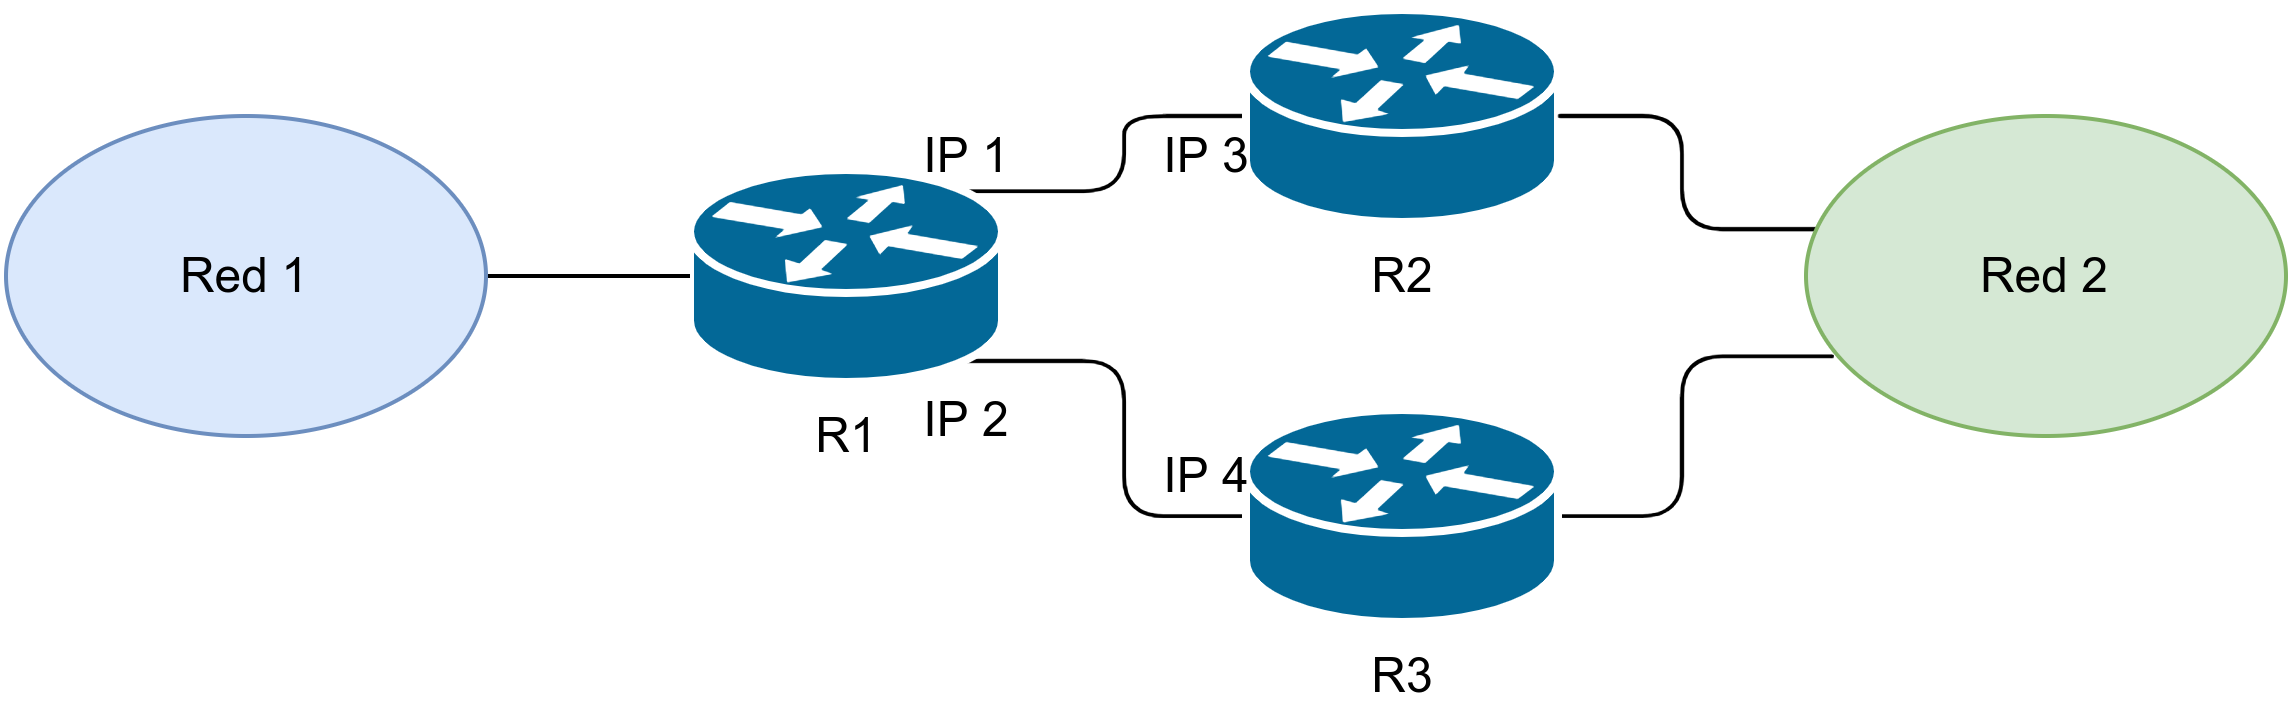
\includegraphics[width=0.8\linewidth]{rutas_estaticas_distancia.png}
    \vspace{-25pt}
\end{center}

Para que la red 1 se pueda comunicar con la red 2 el router R1 puede ir por dos caminos distintos. En este caso, las rutas estáticas a crear serían:
\begin{itemize}
    \item \textbf{Ruta principal}: priorizamos el tráfico por R2, a través de la IP3.
    \item \textbf{Ruta menos prioritaria}: en caso de falla la anterior ruta, el router R1 enviará el tráfico por router R3 llegando a él por la IP4.
\end{itemize}

En este caso, a las rutas menos prioritarias se les añade una “distancia administrativa” (a veces también llamado “peso”). Esta distancia es un número entero que indicará la prioridad (cuanto mayor el número, menor la prioridad).

\subsubsection{Ejemplos}

La creación de rutas estáticas se realiza con \commandbox{ip route RED  MÁSCARA  SALTO} siendo:
\begin{itemize}
    \item \textbf{ip config}: el comando que indica que vamos a crear una ruta.
    \item \textbf{RED}: la  red a la que queremos llegar.
    \item \textbf{MÁSCARA}: Máscara de la red a la que queremos llegar
    \item \textbf{SALTO}: IP del dispositivo a través del cual queremos llegar a la red indicada anteriormente.  Este dispositivo tiene que estar en nuestra misma red y tenemos que poder llegar a él.
\end{itemize}

Por lo tanto, un ejemplo real podría ser:


\begin{mycode}{Crear ruta estática para una red}{powershell}{}
Router(config)# ip route 172.20.10.0  255.255.252.0  10.0.0.2
\end{mycode}

También podemos realizar rutas estáticas sólo para una IP, siendo la máscara /32 en decimal:

\begin{mycode}{Crear ruta estática para un equipo}{powershell}{}
Router(config)# ip route 172.20.10.25  255.255.255.255  10.0.0.3
\end{mycode}

Cuando hay rutas distintas para una IP y una red, se prioriza de lo más específico a lo más genérico. Por lo tanto, se prioriza la ruta de una IP, aunque se indique que para toda la red haya que ir por otro salto.


\subparagraph{Crear ruta estática con “distancia administrativa”}
A la hora de crear una ruta estática con “distancia administrativa”, se realiza de la misma forma que acabamos de ver, pero añadiendo al final la distancia administrativa de la ruta, siendo un número entero. Este “peso” es utilizado cuando en la tabla de rutas existen dos rutas para llegar al mismo destino por caminos diferentes, por lo que se priorizará la ruta con el número más pequeño (o que no tenga número).

\begin{mycode}{Crear ruta estática y ruta con distancia administrativa}{powershell}{}
Router(config)# ip route 172.20.10.0  255.255.252.0  10.0.0.2

Router(config)# ip route 172.20.10.0  255.255.252.0  192.168.1.1  10
\end{mycode}

Como se puede ver, para llegar al mismo destino (172.20.10.0 /22) podemos elegir dos saltos por los que llegar: 10.0.0.2 y 192.168.1.1. La ruta que tenga menor distancia administrativa será la predeterminada, y por tanto los paquetes se irán por ella.


\subsection{Enrutamiento dinámico}

El enrutamiento dinámico permite a los encaminadores ajustar, en tiempo real, los caminos utilizados para transmitir paquetes IP. Cada protocolo posee sus propios métodos para definir rutas (camino más corto, utilizar rutas publicadas por pares, etc.).


\subsubsection{BGP (Border Gateway Protocol)}
El protocolo BGP (en castellano protocolo de “Puerta de Enlace de Frontera”) es un protocolo mediante el cual \textbf{se intercambia información de encaminamiento entre sistemas autónomos}.

%TODO: poner un dibujo de cómo es una red con BGP

Un \textbf{Sistema Autónomo} (o \textbf{AS}, de \textit{Autonomous System}) es un grupo de redes IP controladas por una misma compañía (normalmente un proveedor de internet ISP, o una gran compañía) que son gestionadas de manera independiente y realiza su propia gestión del tráfico. Los sistemas autónomos cuentan con un número (\textbf{ASN}) de 16 o 32 bits que debe ser respetado, ya que al igual que las IPs, existen ASN públicos y privados. En la wikipedia aparece una \href{https://es.wikipedia.org/wiki/Sistema_aut%C3%B3nomo#Tabla_con_ASN_de_16-bit_y_32-bit}{lista de estos rangos}.

El intercambio de esos rangos de IPs se realiza en los denominados “router frontera” o “router externos”, que son los que están comunicados con otros routers de otros AS. Estos routers son los encargados de \textbf{anunciar} las propias redes del AS a sus “vecinos” (neighbors en inglés), que a su vez propagarán esa información a sus propios vecinos ...

Si un AS decide anunciar una nueva red, automáticamente sus vecinos son actualizados, que a su vez propagan la actualización. Si un router recibe su propia actualización, la rechaza.

\errorbox{\textbf{Es importante que un router no anuncie redes IP que no le pertenecen.}}

En la \href{https://en.wikipedia.org/wiki/BGP_hijacking}{wikipedia} aparecen distintos incidentes por errores en la propagación de rutas.
Cuando un router propaga una red (ya sea suya o de otro AS) añade su ASN, y de esta manera se conoce para llegar a una ruta por cuántos AS se pasan (pero no por cuántos routers internos).

Hoy en día Internet funciona con el protocolo BGP y actualmente el protocolo anuncia más de 900.000 rutas (\href{https://blog.apnic.net/2022/01/06/bgp-in-2021-the-bgp-table/}{fuente}):

\begin{center}
    \vspace{-15pt}
    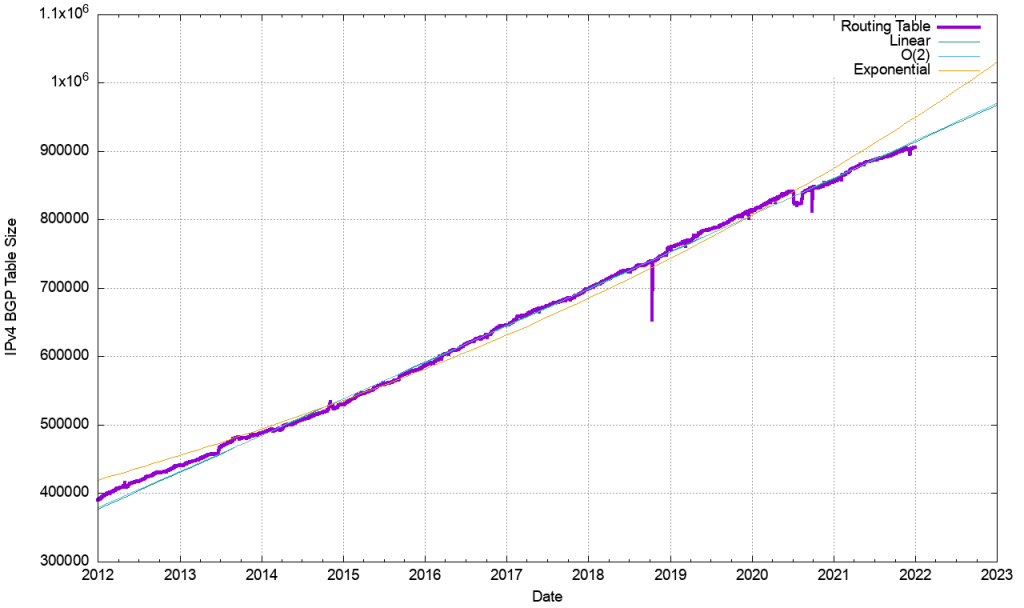
\includegraphics[width=0.8\linewidth]{bgpfig4-1024x608.png}
    \vspace{-25pt}
\end{center}


\subsubsection{Ejemplos}
En los routers debemos crear la configuración para que se convierta en un “\textit{Autonomous System}” (AS, Sistema Autónomo).

\begin{mycode}{Crear sistema autónomo}{powershell}{}
Router(config)# router bgp 100
\end{mycode}

Una vez dentro del sistema autónomo, habrá que indicar qué red se quiere propagar a los “vecinos”:

\begin{mycode}{Anunciar red a propagar}{powershell}{}
Router(config-router)# network 192.168.1.0 mask 255.255.255.0
\end{mycode}

Para poder propagar la red, debemos indicar a qué vecinos se los vamos a propagar:

\begin{mycode}{Vecinos a los que propagar la red}{powershell}{}
Router(config-router)# neighbor 10.10.2.1 remote-as 200
\end{mycode}

Para conocer el estado de las rutas BGP podemos realizar:

\begin{mycode}{Comprobar estado de BGP}{powershell}{}
Router#show ip bgp
BGP table version is 6, local router ID is 192.168.1.1
Status codes: s suppressed, d damped, h history, * valid, > best,
              i - internal, r RIB-failure, S Stale

Origin codes: i - IGP, e - EGP, ? - incomplete

Network               Next Hop           Metric LocPrf  Weight  Path
*> 192.168.1.0/24      0.0.0.0                0     0    32768       i
*> 192.168.2.0/24    10.10.2.1                0     0        0   200 i
\end{mycode}

\subsection{Tabla de rutas completa}
Los routers Cisco tienen una opción que nos muestra todas las rutas a las que el router puede acceder:

\begin{mycode}{Comprobar estado de BGP}{powershell}{{\small}}
Router# show ip route
Codes: C - connected, S - static, I - IGRP, R - RIP, M - mobile, B - BGP
    D - EIGRP, EX - EIGRP external, O - OSPF, IA - OSPF inter area
    N1 - OSPF NSSA external type 1, N2 - OSPF NSSA external type 2
    E1 - OSPF external type 1, E2 - OSPF external type 2, E - EGP
    i - IS-IS, L1 - IS-IS level-1, L2 - IS-IS level-2, ia - IS-IS inter area
    * - candidate default, U - per-user static route, o - ODR
    P - periodic downloaded static route

Gateway of last resort is not set

        8.0.0.0/25 is subnetted, 1 subnets
C       8.8.8.0 is directly connected, GigabitEthernet1/0

        10.0.0.0/30 is subnetted, 1 subnets
C       10.10.0.0 is directly connected, GigabitEthernet2/0

        83.0.0.0/27 is subnetted, 1 subnets
C       83.85.67.0 is directly connected, GigabitEthernet0/0

        95.0.0.0/26 is subnetted, 1 subnets
B       95.94.32.0 [20/0] via 10.10.0.2, 00:00:00

        212.140.23.0/28 is subnetted, 1 subnets
S       212.140.23.16 [1/0] via 83.85.67.4
\end{mycode}

Tal como aparece justo después del comando, hay unos códigos que nos indican si los rangos son:
\begin{itemize}
    \item[\textbf{B:}] Red que podemos llegar mediante el protocolo BGP.
    \item[\textbf{C:}] Red a la que estamos directamente conectados a través de un interfaz físico.
    \item[\textbf{S:}] Red a la que podemos llegar siendo una ruta estática.
\end{itemize}



\chapter{Redes virtuales}
Es habitual querer diferenciar distintas redes dentro de una arquitectura de red (para diferenciar departamentos en una empresa, separar servidores de equipos de trabajo, limitar el acceso entre redes, ...) pero eso supone la compra de distintos equipamientos físicos (distintos switches, puntos de acceso ...) que incrementa el coste de nuestra infraestructura.

Para evitar este incremento de precio, podemos hacer uso de las \textbf{VLAN} en nuestros dispositivos de red, ya sea en switches o en routers, que los soporten.

\section{VLAN}
Una VLAN, acrónimo de \textit{virtual LAN} (red de área local virtual), \textbf{es un método para crear redes lógicas independientes dentro de una misma red física}. Varias VLAN pueden coexistir en un único switch físico o en una única red física, y el tráfico estará separado entre distintas VLANs a nivel lógico.

Un equipo de una VLAN no se podrá comunicar con otro equipo de otra VLAN distinta salvo que haya un router que esté conectado en ambas VLANs y que encamine el tráfico de una a la otra. Lo mismo que si fuesen dos redes físicas, como hemos visto hasta ahora.

Las VLANs se diferencian a través de una cabecera extra la cual se añade dentro del encabezado original de la trama (\textbf{capa 2}). Esa cabecera consta de dos partes de 16 bits, siendo los últimos 12 los que correspondan al valor que identificará a la VLAN, y estará comprendido entre 1 y 4095, ya que el 0 está reservado. Esa cabecera indicará que el tráfico está etiquetado o “\textit{\textbf{tagged}}”.

\infobox{Las VLANs se diferencian a través de una cabecera extra la cual se añade dentro del encabezado original de la trama (\textbf{capa 2}).}

A continuación se puede ver cómo se muestra tráfico etiquetado mediante las cabeceras del \textbf{protocolo 802.1Q}:

\begin{center}
    \vspace{-10pt}
    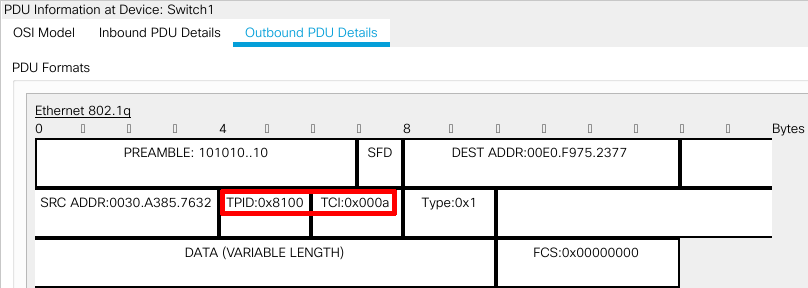
\includegraphics[frame,width=0.9\linewidth]{vlan-tag.png}
    \vspace{-10pt}
\end{center}

\begin{itemize}
    \item \textbf{TPID}: 16 bits en el que el valor  “\textbf{0x8100}” indica que es una trama etiquetada del protocolo \textbf{802.1Q}.
    \item \textbf{TCI}: 16 bits (formando 4 caracteres en hexadecimal):
    \begin{itemize}
        \item \textbf{PCP}: 3 bits que permiten priorizar el tráfico.
        \item \textbf{DEI}: 1 bit, en conjunto con PCP, que permite saber si esta trama se puede descartar en caso de congestión.
        \item \textbf{VID}: \textit{VLAN IDentificator}, 12 bits ($2^{12} = 4096$). En este caso los últimos 3 caracteres hexadecimales “00A” que indica que es la VLAN 10.
    \end{itemize}
\end{itemize}

Hay que tener en cuenta que aunque existe el límite de 4096 VLANs, algunos switches tienen una limitación de un número menor de VLANs activas. Es decir, puedes crear VLANs con el dígito que quieras (hasta 4095), pero quizá sólo te dejan crear 16 VLANs. Ejemplo de la limitación del número de VLANs que puede haber activas en switches “\href{https://www.cisco.com/c/dam/en/us/products/collateral/switches/small-business-100-series-unmanaged-switches/data_sheet_c78-634369_Spanish.pdf}{Cisco de la serie 200 Cisco Small Business}”:

\begin{table}[H]
    \centering
    \begin{tabular}{|L{0.1\linewidth}|L{0.84\linewidth}|}
        \tbody
        VLAN & Compatibilidad con hasta \textbf{256 VLAN simultáneas} (de 4096 ID de VLAN). \textbf{16 VLAN compatibles en SG200-08 y SG200-08P}. VLAN basadas en puertos y en etiquetas 802.1Q
        \\ \hline
        VLAN de voz & El tráfico de voz se asigna automáticamente a una VLAN específica de voz y se trata con los niveles apropiados de QoS
        \\ \hline
    \end{tabular}
    \vspace{-15pt}
\end{table}

Como se puede apreciar, en este modelo de Switch, el límite es de 256 VLAN activas (aunque se puede elegir el ID de la VLAN de las 4096 posibles), y de “sólo” 16 VLANs en el modelo de 8 bocas ethernet de esa serie.


\subsection{Diferencia de arquitecturas con y sin VLANs}
Para que quede más claro lo explicado hasta ahora, vamos a analizar una misma infraestructura de red separada a nivel físico y separada a nivel lógico mediante VLANs.

\subsubsection{Arquitectura sin VLAN}
En una arquitectura de red sin VLANs tendríamos que tener tantos switches como sean necesarios para realizar una separación física de las redes. Estos switches estarán conectados a un router que será el encargado de encaminar el tráfico entre las redes. La separación física de redes es más cara ya que se necesita más hardware y es posible que los switches estén infrautilizados.

\begin{center}
    \vspace{-15pt}
    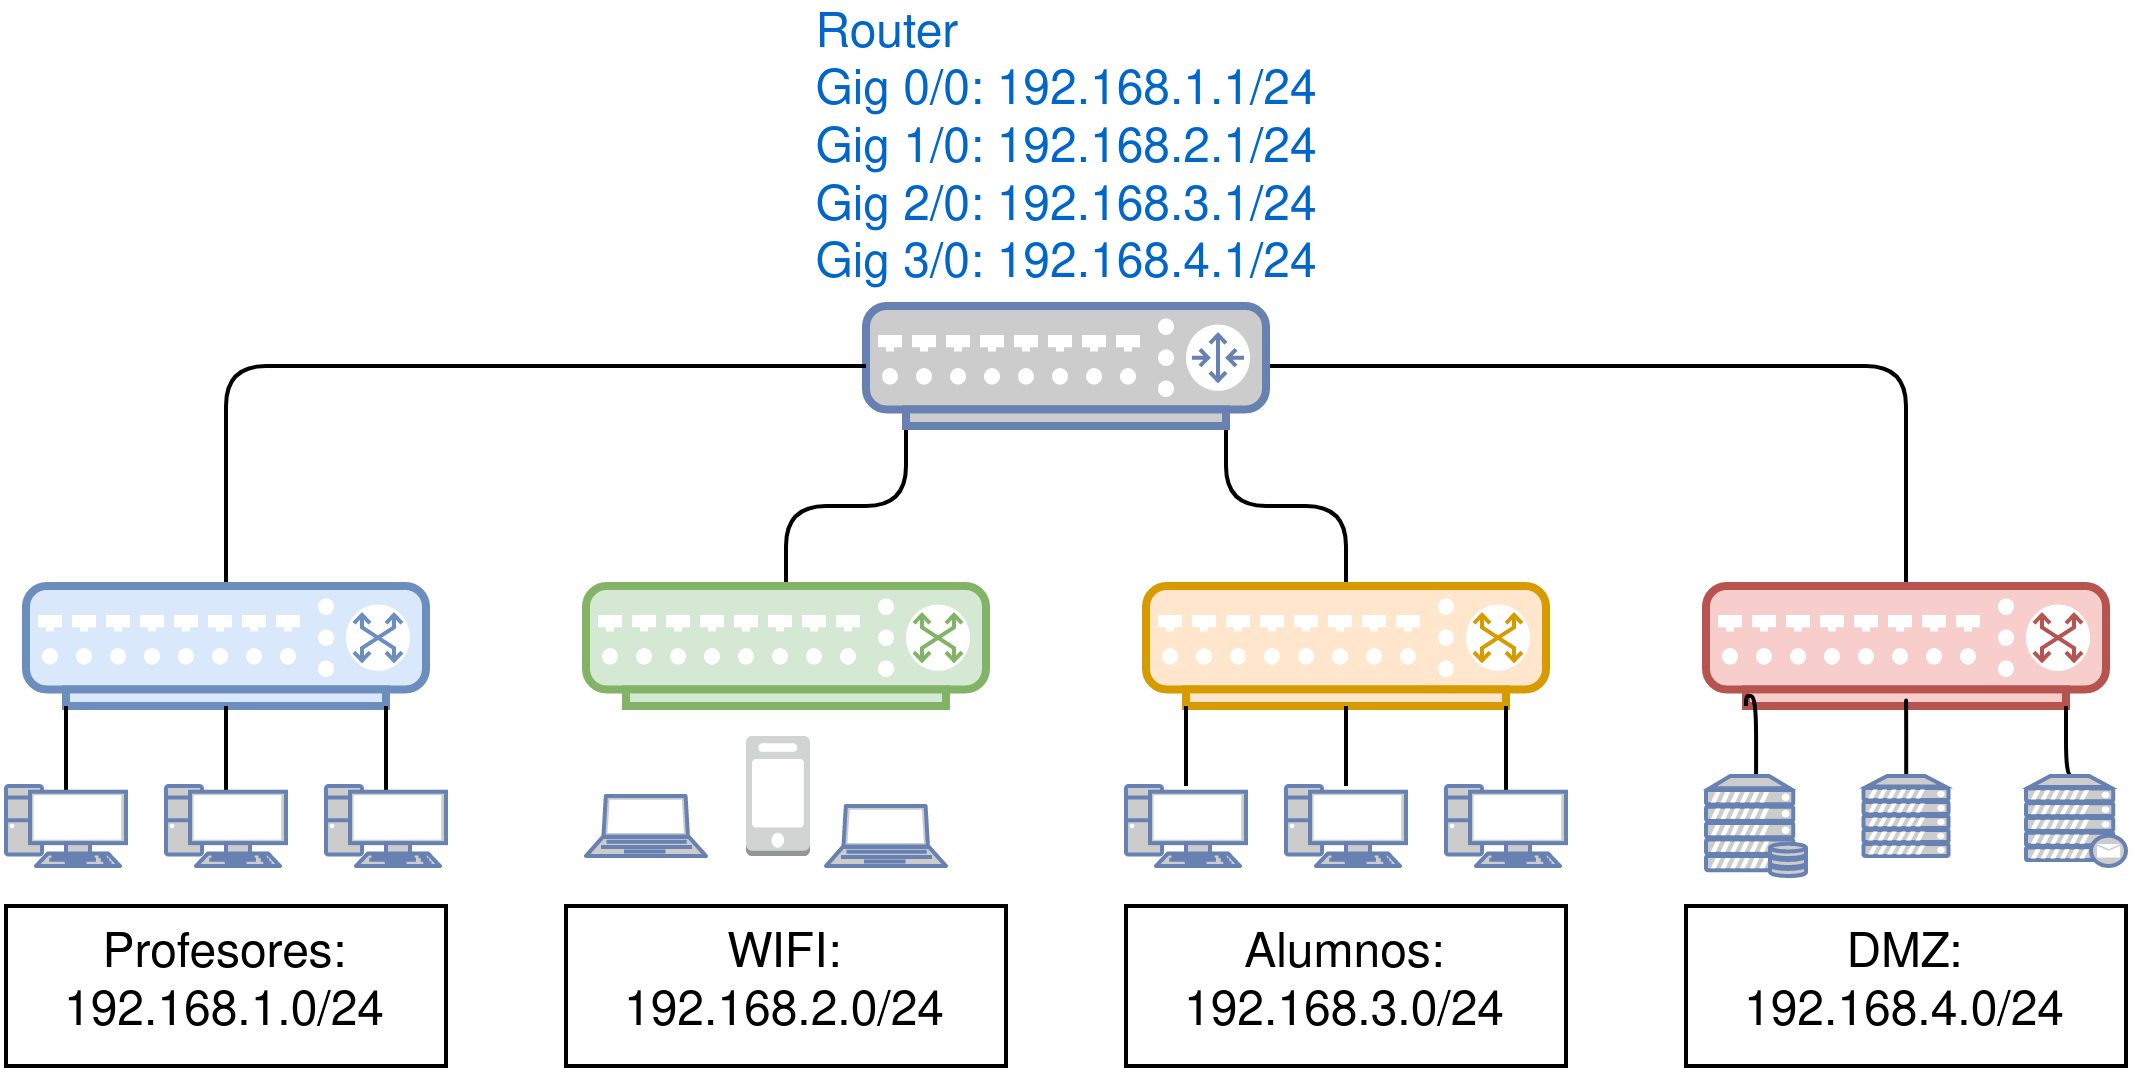
\includegraphics[width=0.8\linewidth]{red-sin-vlan.png}
    \vspace{-15pt}
\end{center}

Se puede observar una arquitectura en la que un router actúa de intermediación en una red en la que existen 4 redes separadas físicamente mediante distintos switches. Si en una red existen pocos dispositivos, el switch de esa red estará infrautilizado. Si por el contrario necesitamos ampliar alguna de las redes, deberemos añadirle un switch en cascada en la red correspondiente, pero aún así ese nuevo switch podría estar infrautilizado.


\subsubsection{Arquitectura con VLANs}

En una arquitectura con \textbf{VLAN}s, tendremos un router que estará conectado a un switch mediante un enlace \hyperlink{puerto_trunk}{trunk}, y en este switch se configurará cada interfaz en modo \hyperlink{puerto_access}{access} teniendo en cuenta el dispositivo que se vaya a conectar a dicha interfaz. En caso de necesitar ampliar las redes, se hará uso de las interfaces no utilizadas, y en caso de no haber más, el switch se podría expandir añadiendo uno nuevo y \hyperlink{stack_switches}{creando un stack} entre ellos.

\begin{center}
    \vspace{-15pt}
    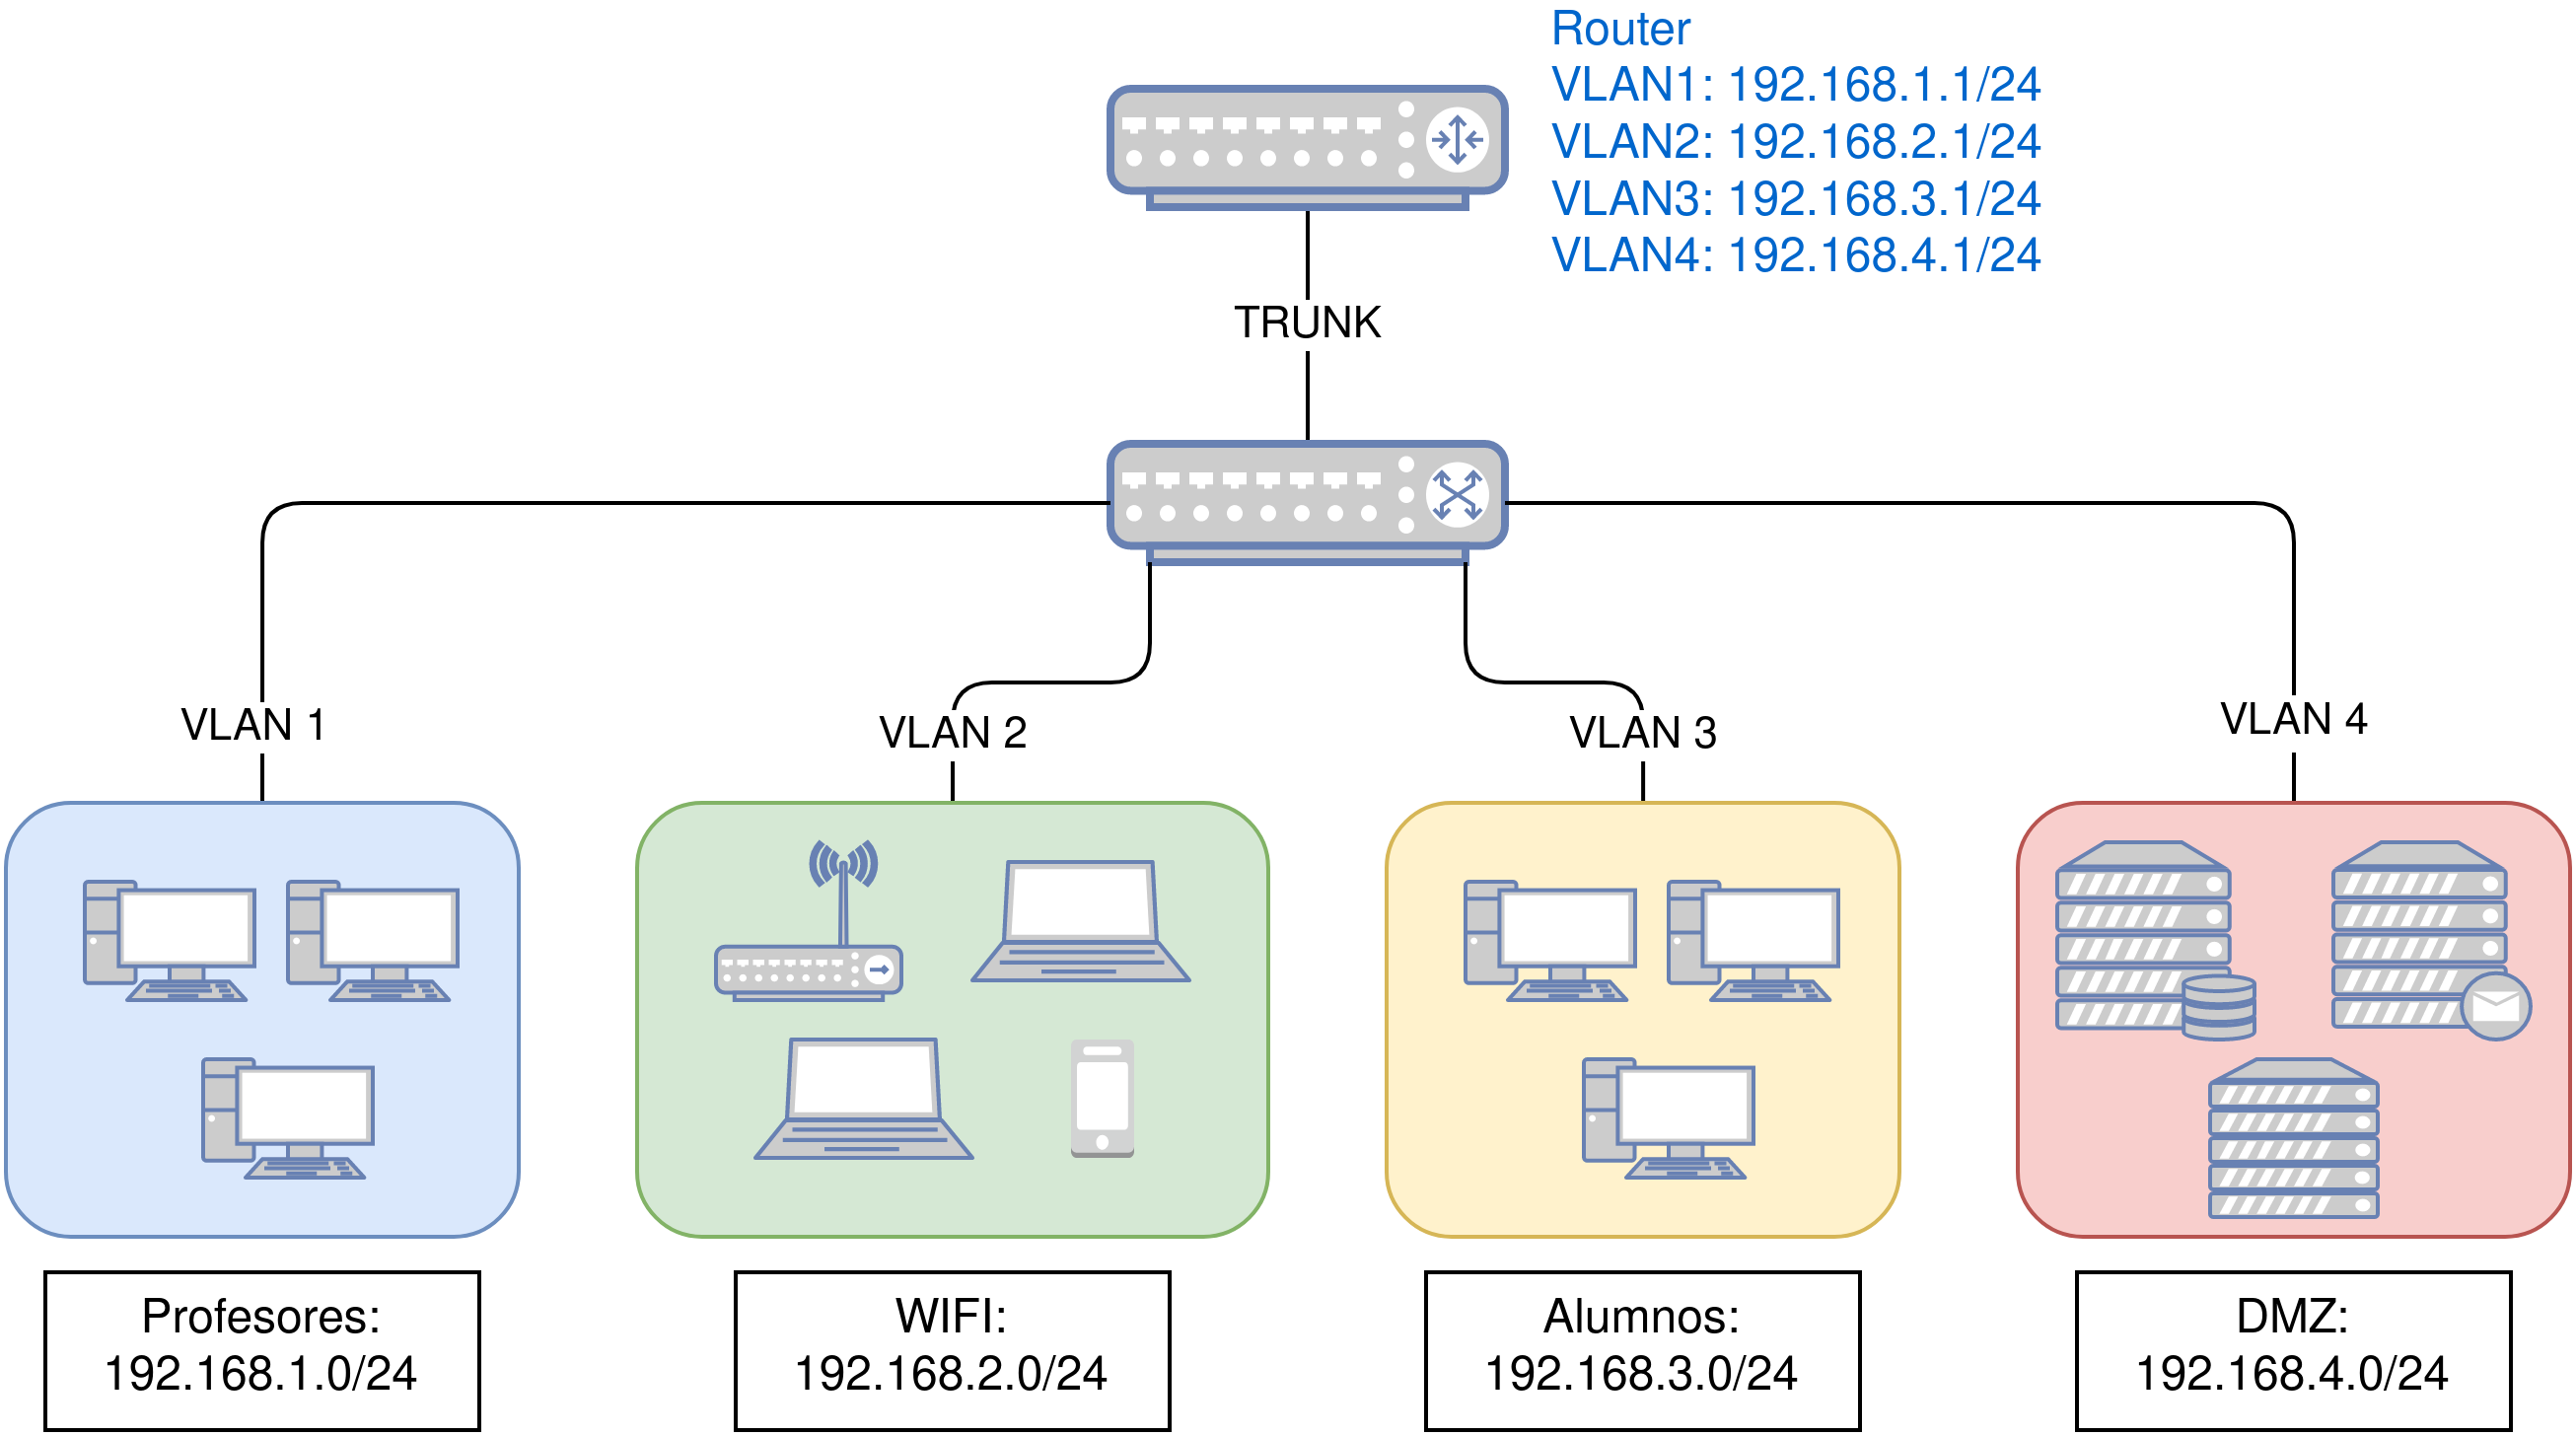
\includegraphics[width=0.8\linewidth]{red-con-vlan.png}
    \vspace{-15pt}
\end{center}

\section{VLANs en Switches}

En los switches se pueden realizar distintas configuraciones teniendo en cuenta las VLANs que vayamos a utilizar y la arquitectura de red que tengamos:

\begin{itemize}
    \item \textbf{VLAN por defecto en el switch}: Es la VLAN en la que trabajará el switch. Por defecto suele ser la \textbf{VLAN 1}. El tráfico por defecto va en esa VLAN y para ir por cualquier otra VLAN el tráfico deberá estar “\textit{tagged}” (etiquetado).

    \hypertarget{puerto_trunk}{}
    \item \textbf{Puerto en modo “\textit{trunk}”}: Normalmente utilizado para comunicación entre distintos switches y/o routers. A este enlace “\textbf{\textit{trunk}}” (o troncal, o tronco) se le asigna una VLAN por defecto y las VLANs “\textbf{tagged}” permitidas que pasarán por él. Los switches sabrán a qué VLAN pertenece cada trama observando la etiqueta VLAN de la capa 2.

    El tráfico que \textbf{entra} en esta boca, si no está etiquetado estará en la VLAN por defecto. Si está etiquetado en una VLAN permitida se permitirá el tráfico.

    El tráfico que \textbf{sale} de esta boca saldrá de la misma manera con la que llegó a él (sin etiquetar o etiquetado con la VLAN que sea). El equipo que reciba esta trama tendrá que lidiar con el tráfico recibido (ya sea etiquetado o no).

    \hypertarget{puerto_access}{}
    \item \textbf{Puerto en modo “\textit{access}”}: La boca del switch se define en modo “access” (o “acceso”) y se le asigna una \textbf{única VLAN} a la misma.

    Este tipo de configuraciones suele ser utilizada para conectar equipos en los que no podemos etiquetar VLANs en origen (impresoras por ejemplo), o nos resulte tedioso la configuración de la misma, pero queremos asegurar que su tráfico viaje por una VLAN.

    El \textbf{tráfico que entra} en esta boca, a partir de ese momento \textbf{se le añadirá la cabecera de la VLAN a la trama} convirtiéndose en tráfico “tagged”.

    Si el \textbf{tráfico sale} de una boca en modo “access” se quitará la cabecera VLAN, por lo que \textbf{al equipo remoto le llegará el tráfico sin estar “tagged”}.

\end{itemize}

Teniendo en cuenta lo explicado previamente, se puede observar en el siguiente dibujo en el que aparecen varios switches, configurados con distintas bocas en modo \textbf{access} y otras en modo \textbf{trunk}. Como se puede ver, las bocas que comunican los distintos dispositivos (switches con switches y switch con router) están configuradas en modo TRUNK, y en ellas se permiten varias VLANs.

Las interfaces que sólo tienen un color, están configuradas en modo \textbf{access} con una VLAN. Los interfaces en blanco no están configurados (ya que usan la VLAN por defecto, en este caso la VLAN 1). Para que el router pueda enrutar las distintas redes, le tendrán que llegar a través de un enlace configurado en modo \textbf{trunk}.
\textbf{}

\begin{center}
    \vspace{-10pt}
    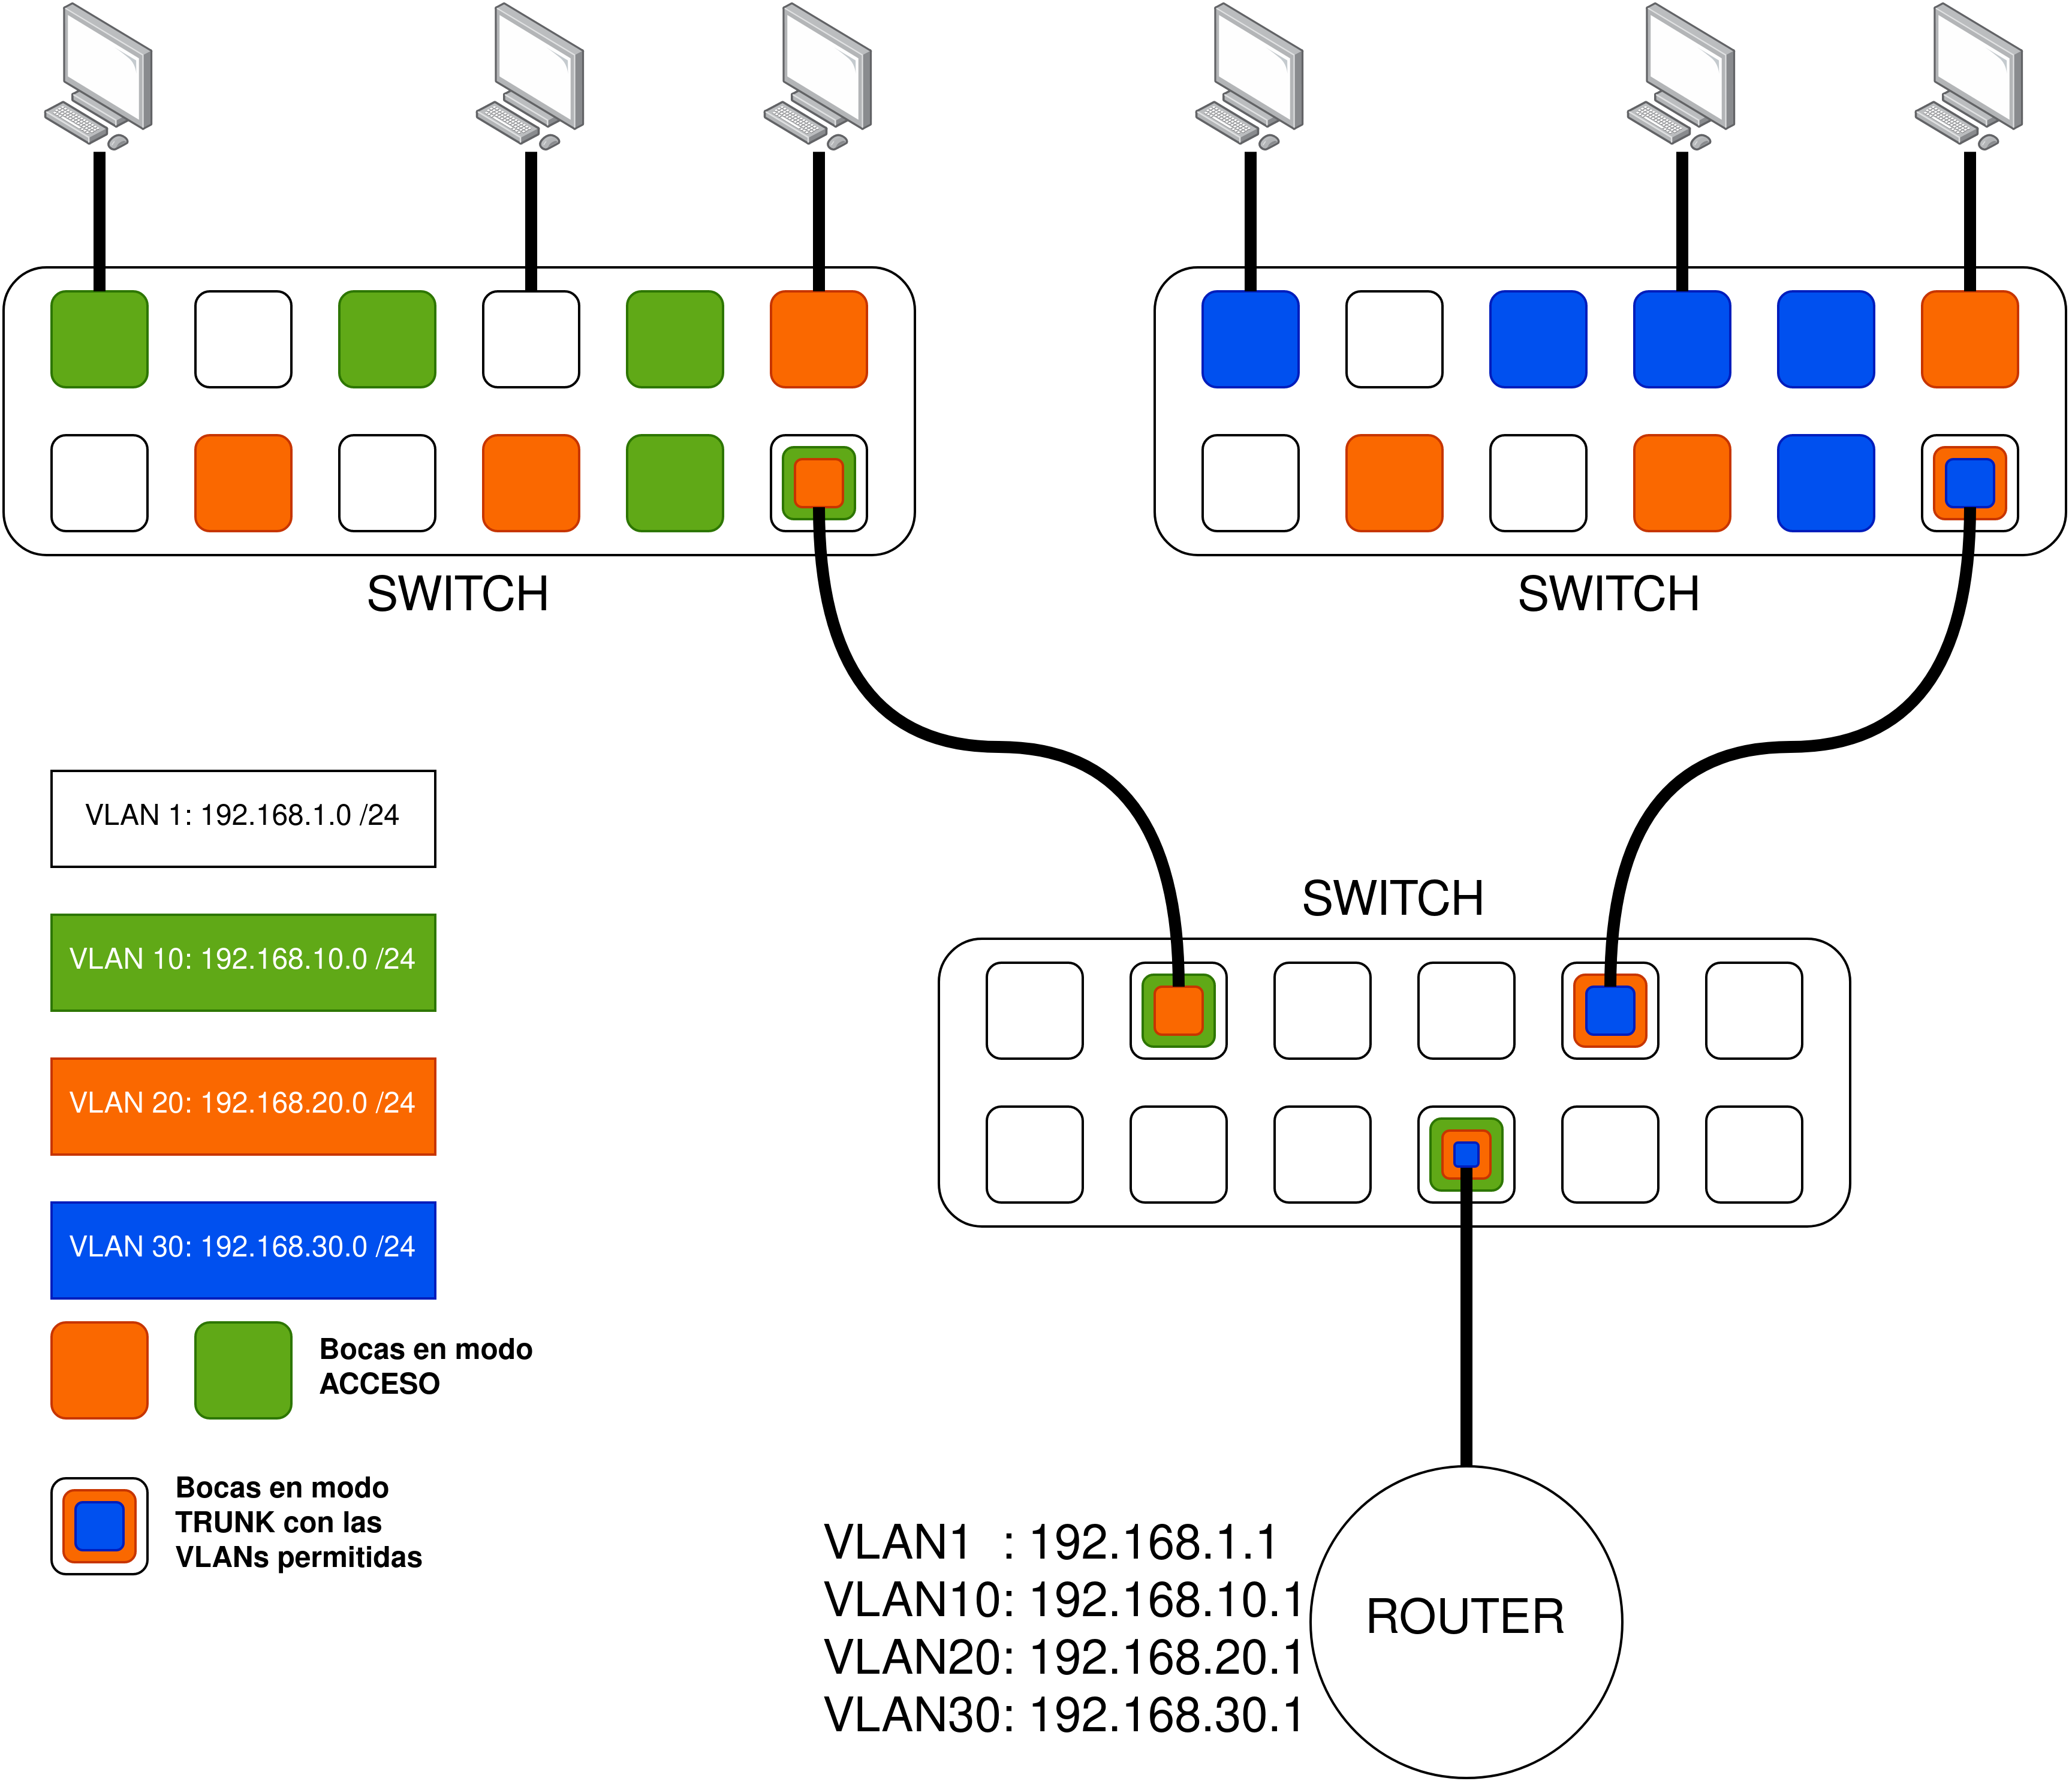
\includegraphics[width=0.9\linewidth]{switch_configuracion_access_trunk.png}
    \vspace{-10pt}
\end{center}


\subsection{Crear VLAN}
Para crear una VLAN primero deberemos identificar el identificador, y luego suele ser recomendable darle un nombre identificativo.

\begin{mycode}{Crear VLAN}{powershell}{}
Switch(config)# vlan 10
Switch(config-vlan)# name Profesores
\end{mycode}

\subsection{Añadir IP en una VLAN}
En caso de necesitarlo, se podrá añadir una IP a cada nueva vlan que se haya creado, tal como se hace con la VLAN 1, pero eligiendo la VLAN correspondiente.

\begin{mycode}{Añadir IP a la VLAN}{powershell}{}
switch(config)# interface vlan10
switch(config-if)# ip address 10.10.0.254 255.255.255.0
switch(config-if)# no shutdown
\end{mycode}

\subsection{Listar tabla de VLAN}
El siguiente comando nos muestra la base de datos interna de VLANs que tiene el switch, indicando el estado y un pequeño resumen de en qué bocas está activa. Hay que tener en cuenta que no nos indica en qué modo está configurada dicha VLAN en cada interfaz, por lo que deberemos comprobarlo mirando detalladamente la configuración completa.

\begin{mycode}{Listar la tabla de VLAN}{powershell}{}
Switch# show vlan

VLAN    Name            Status    Ports
---- ------------------ --------- --------
1    default            active    Gig1/1
10   profesores         active    Gig0/1
20   alumnos            active
...
\end{mycode}

También hay que tener en cuenta que aunque un interfaz esté configurado con una VLAN, si no aparece en la base de datos, es como si no existiese.

\subsection{Configurar interfaz con VLAN en acceso}
Para configurar un interfaz en modo \textbf{\textit{access}} tendremos que elegir primero el interfaz y después elegir el modo a configurar y para qué VLAN. Es importante haber creado primero la VLAN.
\begin{mycode}{Configurar interfaz en modo trunk}{powershell}{}
Switch(config)# interface GigabitEthernet 0/1
Switch(config-if)# switchport mode access
Switch(config-if)# switchport access vlan 10
\end{mycode}


\subsection{Configurar interfaz con VLAN en trunk}
Para configurar un interfaz en modo \textbf{\textit{trunk}} tendremos que elegir primero el interfaz y después elegir el método de configuración:

\begin{mycode}{Configurar interfaz en modo trunk}{powershell}{}
Switch (config)# interface GigabitEthernet 1/1
Switch(config-if)# switchport mode trunk
Switch(config-if)# switchport trunk allowed vlan  ???
\end{mycode}

Donde “???” pueden ser varias opciones:
\begin{itemize}
    \item \textbf{add}: add VLANs to the current list
    \item \textbf{all}: all VLANs
    \item \textbf{except}: all VLANs except the following
    \item \textbf{none}: no VLANs
    \item \textbf{remove}: remove VLANs from the current list
\end{itemize}
Podemos poner la VLAN por defecto en una boca en modo trunk con:

\begin{mycode}{Poner vlan por defecto en un trunk}{powershell}{}
Switch(config-if)# switchport trunk native vlan 10
\end{mycode}


\subsection{VLANs en Routers}
En los routers, las VLANs van asociadas a una interfaz física. Al añadir una VLAN, se crea una interfaz “virtual”, y dentro se le indica que va a ser de tipo “\textbf{encapsulation dot1Q}” y la VLAN que va a usar. Después, se le configura la IP como si fuera una interfaz normal. Como ejemplo para la VLAN 20:

\begin{mycode}{Crear VLAN 20 en Router y configurar una IP}{powershell}{}
Router(config)# interface GigabitEthernet0/0.20
Router(config-if)# encapsulation dot1Q 20
Router(config-if)# ip address 192.168.20.1 255.255.255.0
\end{mycode}




\subsection{VLANs en servidores/ordenadores}
El tráfico que “sale” de un servidor/ordenador, por defecto, no está etiquetado con ninguna VLAN. En caso de que queramos que el tráfico saliente salga con una VLAN etiquetada, tendremos que configurar el interfaz de red para que funcione con dicha VLAN.



\section{Protocolo VTP}
VTP, o \textbf{VLAN Trunk Protocol}, es un protocolo que nos permite configurar y administrar VLANs en equipos Cisco de manera centralizada. De esta manera conseguimos simplificar la tarea cuando tenemos una red en la que disponemos de muchas VLANs

El protocolo funciona en modo  servidor-cliente, por lo tanto debemos configurar un switch en modo servidor, que será en el que realizaremos la administración de las VLANs, que posteriormente serán propagadas por los switches que son clientes VTP y que pertenecen al mismo dominio.


\warnbox{La conexión entre switches debe estar en modo \textbf{trunk} para que el protocolo funcione de manera correcta.}

\subsection{Configurar switch como VTP Server}
Es tan fácil como elegir el modo servidor del protocolo VTP, indicar un dominio de propagación y una contraseña para el mismo.

\begin{mycode}{Crear configuración como VTP Server}{powershell}{}
Switch(config)# vtp mode server
Switch(config)# vtp domain instituto
Switch(config)# vtp password 1234
\end{mycode}

\subsection{Configurar switch como VTP Client}
Similar al caso anterior, pero esta vez eligiendo que queremos que el switch sea cliente:

\begin{mycode}{Crear configuración como VTP Client}{powershell}{}
    Switch(config)# vtp mode client
    Switch(config)# vtp domain instituto
    Switch(config)# vtp password 1234
\end{mycode}

\subsection{Ver estado de VTP}
Para comprobar el estado del servicio VTP, tanto en un switch que sea \textit{server} o \textit{client}:

\begin{mycode}{Ver configuración de estado de VTP}{powershell}{}
Switch# show vtp status

VTP Version                     : 2
Configuration Revision          : 2
Maximum VLANs supported locally : 255
Number of existing VLANs        : 7
VTP Operating Mode              : Server
VTP Domain Name                 : instituto
VTP Pruning Mode                : Disabled
VTP V2 Mode                     : Disabled
VTP Traps Generation            : Disabled
MD5 digest                      : 0x68 0x70 0x3B 0xF0 0x14 0xC8 0xF7 0xE9
Configuration last modified by 0.0.0.0 at 3-1-93 00:11:38
Local updater ID is 0.0.0.0 (no valid interface found)
\end{mycode}

Y nos ofrece un resumen del estado del mismo.



\chapter{Alta Disponibilidad en sistemas de red}
La \hyperlink{altadisponibilidad}{Alta Disponibilidad} en una arquitectura de red es vital si queremos asegurar el acceso a otras redes o servicios. Para ello podemos hacer uso de distintas tecnologías que nos ayudarán a conseguirlo.



\section{Agregación de enlaces: Etherchannel / LACP}
La agregación de enlaces consiste en combinar (agregar) varias conexiones en paralelo para aumentar el \textit{\textbf{throughput}} (la tasa de transferencia) que conseguiría una única conexión. Un grupo de agregación de enlaces (\textbf{LAG}, de \textit{Link Aggregation Group}) combina una serie de puertos físicos de manera que se consigue una única ruta con más ancho de banda que un único enlace.

A lo largo de los años ha habido distintos estándares para la creación de agregación de enlaces. El último es el conocido como \textbf{LACP} (\textit{Link Aggregation Control Protocol}), que provee un método para controlar la unión de varios puertos físicos formando un único canal lógico. LACP permite negociar automáticamente la unión entre dispositivos mediante el envío de paquetes LACP al otro dispositivo.
LACP permite el modo:

\begin{itemize}
    \item \textbf{activo}: Habilita LACP de manera incondicional. Esto puede hacer que si en las bocas que están habilitadas en modo LACP se conecta algo que no está configurado para ello, no funcione de manera correcta
    \item \textbf{pasivo}: Habilita LACP sólamente cuando se detecta un dispositivo configurado con LACP
\end{itemize}

Como ya se ha comentado, la finalidad es la de unir distintas conexiones para aumentar la tasa de transferencia, y esto no sólo se puede realizar entre switches, si no que también se puede realizar entre un switch y un servidor.

A continuación podemos ver cómo sería un sistema LACP entre dos switches.

\begin{center}
    \vspace{-10pt}
    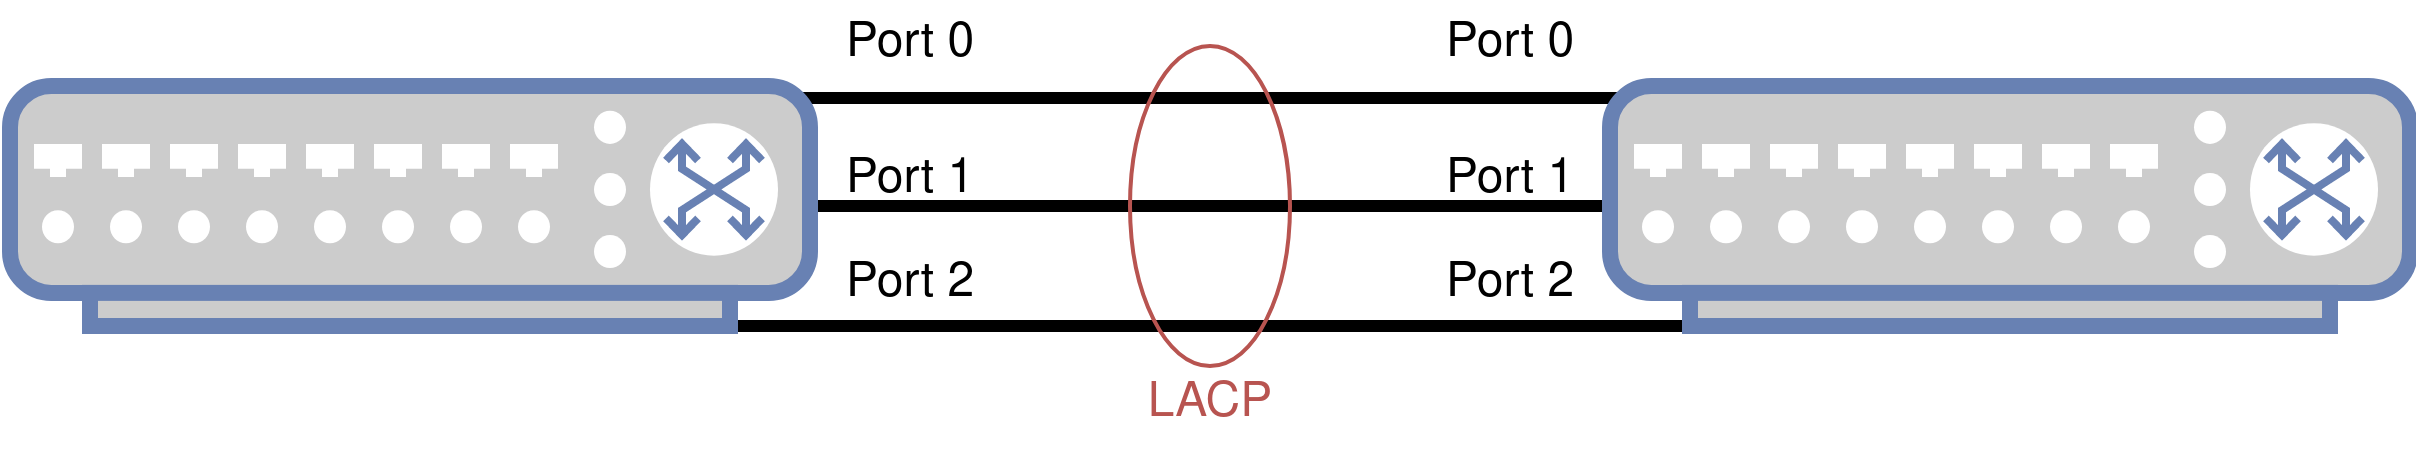
\includegraphics[width=0.7\linewidth]{LACP-switches.png}
    \vspace{-10pt}
\end{center}

Y aquí podemos ver cómo sería una agregación de enlaces entre un switch y un servidor (ya que en un servidor también podemos realizar la agregación de enlaces).

\begin{center}
    \vspace{-10pt}
    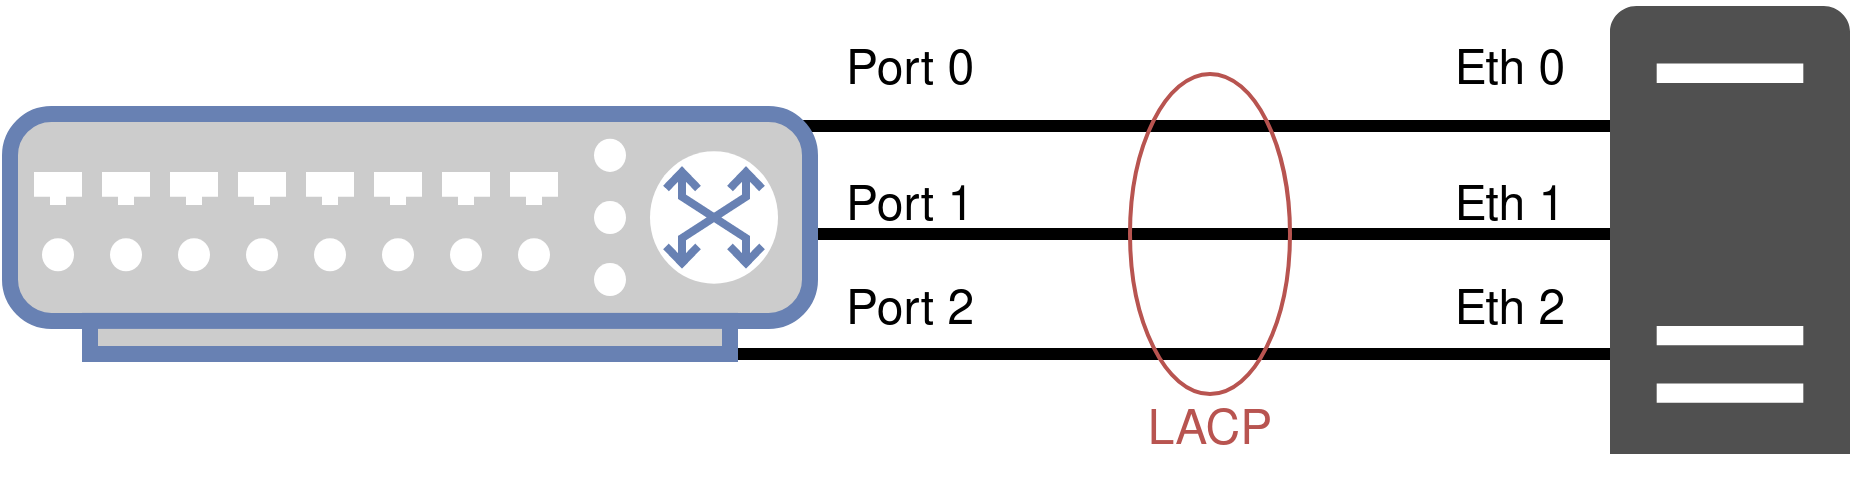
\includegraphics[width=0.6\linewidth]{LACP-switch-server.png}
    \vspace{-10pt}
\end{center}


\subsection{Configurar Etherchannel en Switches}
Antes de realizar ninguna configuración, debemos pensar qué interfaces queremos combinar en una agregación formada por el protocolo LACP.

Para realizar la configuración, deberemos entrar en cada interfaz y añadirlo a un channel-group (siendo el identificador entre el número 1 y el 6) y activar el protocolo a usar:


\begin{mycode}{Añadir interfaces a un \textbf{LAG}}{powershell}{}
Switch(config-if)# channel-group 1 mode active
Switch(config-if)# channel-protocol lacp
\end{mycode}

Cuando se crea un grupo de agregación de enlaces se crea un nuevo interfaz llamado “\textbf{Port-Channel}” (abreviado como “\textbf{Po}”). Es decir, si hacemos la agregación de enlaces con las bocas “0/1” y “1/1” del switch para generar un “channel-group 1”, el switch generará una boca nueva llamada “Port-Channel 1”, la cual podrá ser configurada para hacer lo que necesitemos. En Packet Tracer se pueden tener hasta 6 port-channels:

\begin{mycode}{Configurar Port-Channel 1 en modo \textbf{trunk}}{powershell}{}
switch(config)# interface Port-Channel 1
switch(config-if)# switchport mode trunk
\end{mycode}


Para poder ver el estado del etherchannel/agregación de enlaces:

\begin{mycode}{Ver el estado de los etherchannels}{powershell}{}
Switch# show etherchannel summary

Flags:  D - down        P - in port-channel
I - stand-alone s - suspended
H - Hot-standby (LACP only)
R - Layer3      S - Layer2
U - in use      f - failed to allocate aggregator
u - unsuitable for bundling
w - waiting to be aggregated
d - default port

Number of channel-groups in use: 2
Number of aggregators:           2

Group  Port-channel   Protocol   Ports
------+-------------+-----------+--------------------
1      Po1(SU)           LACP     Gig0/1(P) Gig1/1(P)
2      Po2(SU)           LACP     Gig2/1(P) Gig3/1(P)
\end{mycode}

En este ejemplo, el switch tiene dos agregaciones de enlaces creadas, dos port-channels:
\begin{itemize}
    \item \textbf{Po1}: Tiene configurados los interfaces: Gig 0/1 y Gig 1/1.
    \item \textbf{Po2}: Tiene configurados los interfaces: Gig 2/1 y Gig 3/1.
\end{itemize}

\warnbox{Cada interfaz de cada agregación de enlaces tiene que aparecer con un “\textbf{(P)}”.
    Eso significa que pertenece al port-channel y está correcto.
}


\hypertarget{stack_switches}{}
\section{Stack de switches}

\begin{wrapfigure}{r}{0.36\linewidth}
    \centering
    \vspace{-40pt}
    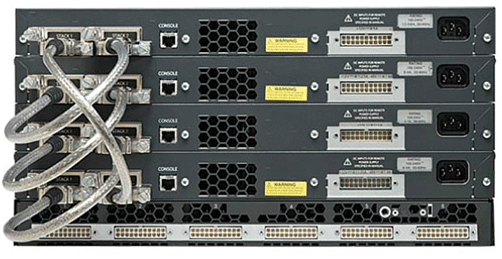
\includegraphics[width=\linewidth]{stack_fisico.png}
    \vspace{-32pt}
    \captionof{figure}{Stack mediante cables especiales}
    \vspace{-30pt}
\end{wrapfigure}
De manera resumida, es la configuración aplicada a varios switches para que actúen como uno sólo. Esto se realiza mediante la interconexión de los switches (formando un anillo) a través de unos puertos especiales o unas conexiones habilitadas para ello.

Tras la realización del “stackado” de switches las ventajas que obtendremos son muy significativas:

\begin{itemize}
    \item Podremos configurar todas las bocas del conjunto de todos los switches que lo forman desde un único punto central (ya sea mediante el CLI o mediante la web de gestión).
    \item Tendremos redundancia en las comunicaciones.
    \item Permite escalar el tamaño de las comunicaciones y podríamos añadir más switches en un momento dado (algunas marcas permiten 12 switches en un mismo stack).
\end{itemize}

Hay que tener en cuenta que no todos los switches permiten realizar un stack de switches, por lo que tendríamos que asegurarnos que si vamos a necesitar esta funcionalidad, a la hora de comprar los switches lo soporten.

\begin{center}
    \vspace{-10pt}
    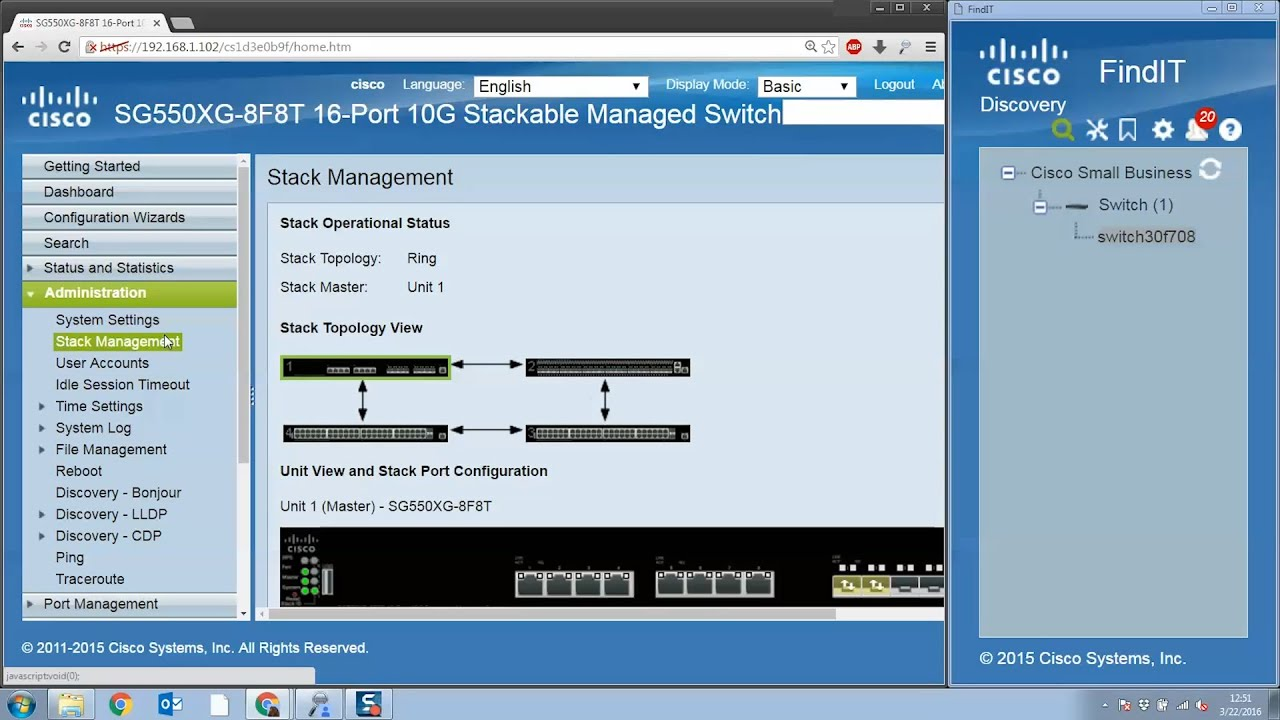
\includegraphics[frame,trim={5 255 572 75},clip,width=0.6\linewidth]{stack_cisco.jpg}
    \vspace{-10pt}
\end{center}


\subsection{Integración de Stack y LACP}
Si realizamos la combinación de configuraciones de Stack de switches junto con LACP con servidores, nos aseguraremos de tener una Alta Disponibilidad real en lo que se refiere a comunicaciones.

Veamos el siguiente dibujo:


\begin{center}
    \vspace{-10pt}
    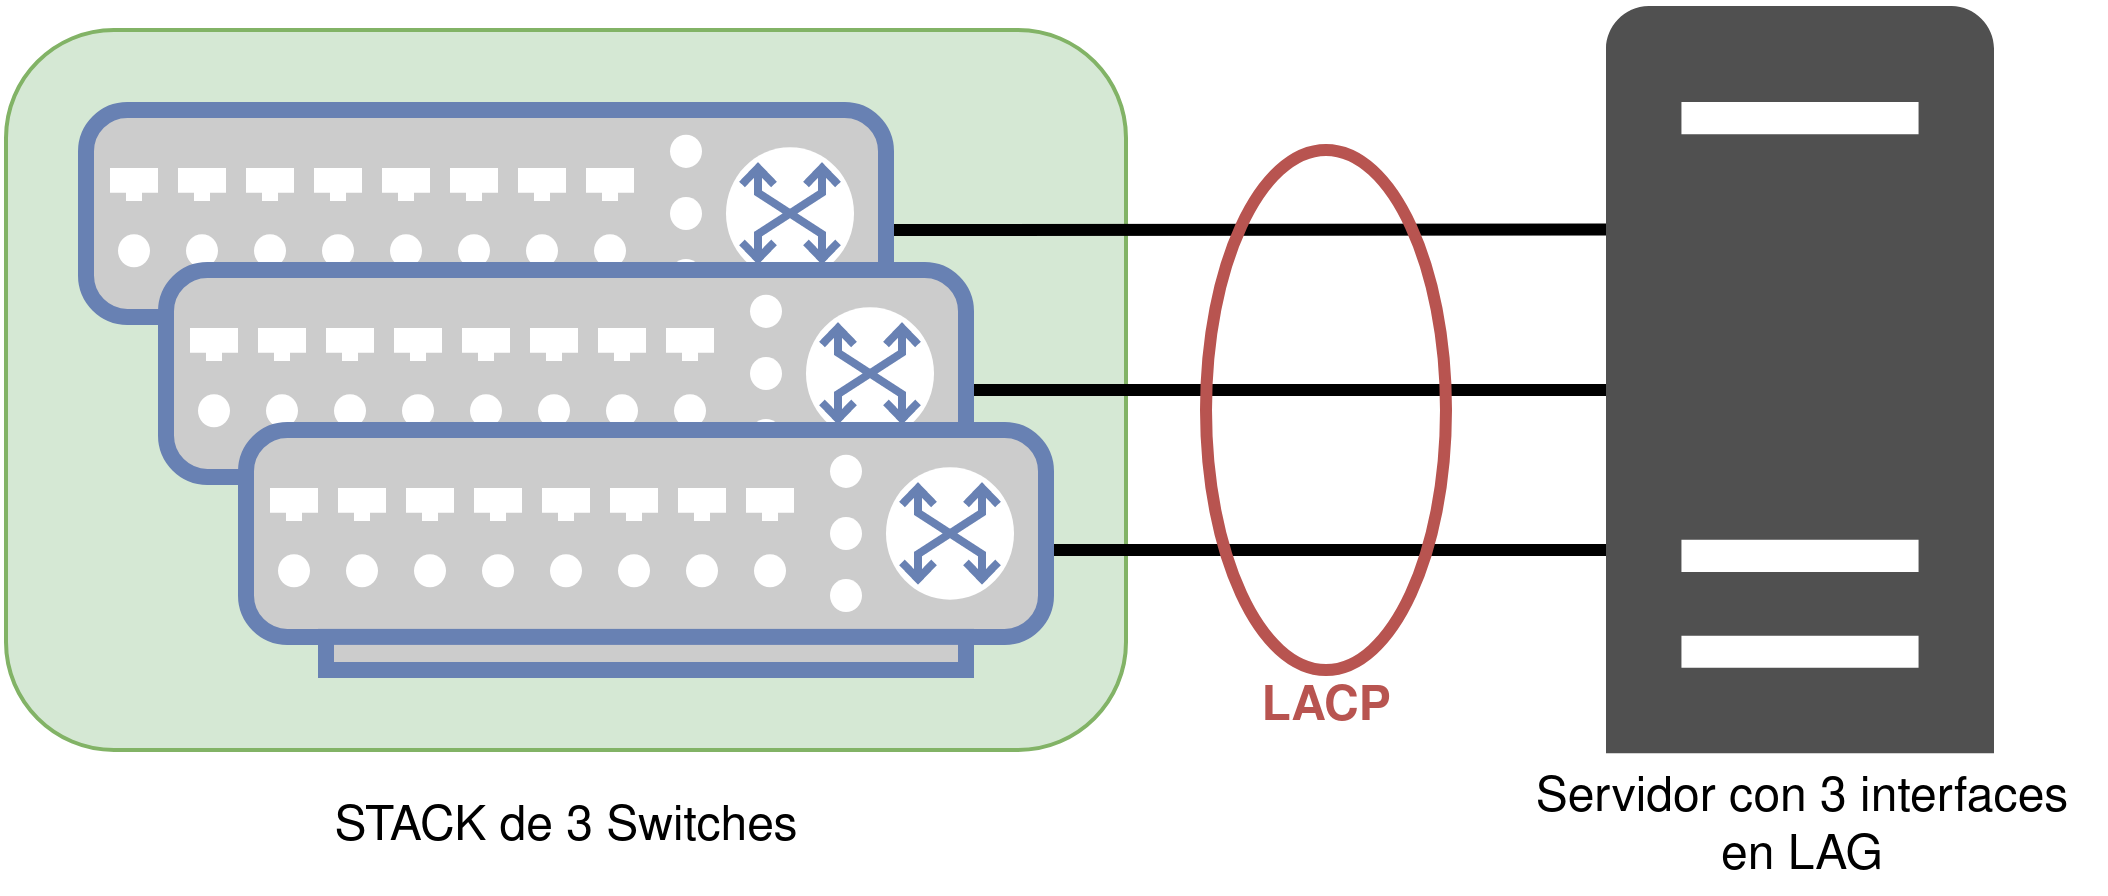
\includegraphics[width=0.6\linewidth]{LACP_stack_servidor.png}
    \vspace{-10pt}
\end{center}

Podemos observar cómo tenemos un stack de 3 switches, que como ya hemos visto previamente actúan como si se tratara de uno sólo. Por otro lado tenemos el servidor, que cuenta con 3 tarjetas ethernet que han sido configuradas a nivel de sistema operativo en modo LACP, y cada una de ellas se ha conectado a un switch distinto del stack.

\infobox{Con esta configuración, nos estamos asegurando que si un switch se estropea, la conectividad seguirá existiendo entre el servidor y el stack a través de los dos enlaces restantes.}

Es muy importante que nuestra infraestructura de red sea pensada para tener el menor número puntos de fallos posibles, y haciendo uso de stacks de switches y conexiones LACP podremos reducir esos puntos de fallo.



    \part{Ejercicios}
    \hypertarget{tabla_conversiones_directas}{}

\chapter{Sistemas de numeración: tabla de conversión}
La siguiente tabla sirve a modo de resumen de los sistemas de numeración.

\infobox{\textbf{Esta tabla no hay que aprenderla de memoria}.
    Hay que entender los sistemas de numeración y de esta manera se puede crear. }

\begin{yukitblr}{X X X X}
    Decimal       &      Binario     &      Octal    & Hexadecimal \\

    $  0_{(10} $  & $      0_{(2} $  & $  0_{(8} $   & $  0_{(16} $  \\
    $  1_{(10} $  & $      1_{(2} $  & $  1_{(8} $   & $  1_{(16} $  \\
    $  2_{(10} $  & $     10_{(2} $  & $  2_{(8} $   & $  2_{(16} $  \\
    $  3_{(10} $  & $     11_{(2} $  & $  3_{(8} $   & $  3_{(16} $  \\
    $  4_{(10} $  & $    100_{(2} $  & $  4_{(8} $   & $  4_{(16} $  \\
    $  5_{(10} $  & $    101_{(2} $  & $  5_{(8} $   & $  5_{(16} $  \\
    $  6_{(10} $  & $    110_{(2} $  & $  6_{(8} $   & $  6_{(16} $  \\
    $  7_{(10} $  & $    111_{(2} $  & $  7_{(8} $   & $  7_{(16} $  \\
    $  8_{(10} $  & $   1000_{(2} $  & $ 10_{(8} $   & $  8_{(16} $  \\
    $  9_{(10} $  & $   1001_{(2} $  & $ 11_{(8} $   & $  9_{(16} $  \\
    $ 10_{(10} $  & $   1010_{(2} $  & $ 12_{(8} $   & $  A_{(16} $  \\
    $ 11_{(10} $  & $   1011_{(2} $  & $ 13_{(8} $   & $  B_{(16} $  \\
    $ 12_{(10} $  & $   1100_{(2} $  & $ 14_{(8} $   & $  C_{(16} $  \\
    $ 13_{(10} $  & $   1101_{(2} $  & $ 15_{(8} $   & $  D_{(16} $  \\
    $ 14_{(10} $  & $   1110_{(2} $  & $ 16_{(8} $   & $  E_{(16} $  \\
    $ 15_{(10} $  & $   1111_{(2} $  & $ 17_{(8} $   & $  F_{(16} $  \\
    $ 16_{(10} $  & $  10000_{(2} $  & $ 20_{(8} $   & $ 10_{(16} $  \\
    $ 17_{(10} $  & $  10001_{(2} $  & $ 21_{(8} $   & $ 11_{(16} $  \\
    ... & ... & ... & ... \\
    $ 29_{(10} $  & $  11101_{(2} $  & $ 35_{(8} $   & $ 1D_{(16} $  \\
    $ 30_{(10} $  & $  11110_{(2} $  & $ 36_{(8} $   & $ 1E_{(16} $  \\
    $ 31_{(10} $  & $  11111_{(2} $  & $ 37_{(8} $   & $ 1F_{(16} $  \\
    $ 32_{(10} $  & $ 100000_{(2} $  & $ 40_{(8} $   & $ 20_{(16} $  \\
\end{yukitblr}

\clearpage

    \chapter{Conversiones}

\section{De decimal ...}

\subsection*{... a binario}

\begin{tblr}{XXXX}
    30 =  & 145 =  & 278 =  & 329 = \\
    512 = & 776 =  & 1024 = & 1376 = \\
\end{tblr}


\subsection*{... a octal}
\begin{tblr}{XXXX}
    31 =  & 88 =  & 127 =  & 234 = \\
    524 = & 876 = & 1098 =  & 2475 = \\
\end{tblr}


\subsection*{... a hexadecimal}
\begin{tblr}{XXXX}
    29 =   & 340 =  & 530 =   & 940 = \\
    1212 = & 1512 = & 2120 =  & 3201 = \\
\end{tblr}

\vspace{10pt}
\section{De binario ...}

\subsection*{... a decimal}

\begin{tblr}{XXXX}
    111001 =         & 11001010 =    & 110101101 =     & 1010101101 = \\
    10101010101110 = & 10101111101 = & 111100010110 =  & 111000100110110 = \\
\end{tblr}

\subsection*{... a octal}

\begin{tblr}{XXXX}
    111001 =         & 11001010 =    & 110101101 =    & 1010101101 = \\
    10101010101110 = & 10101111101 = & 111100010110 =  & 111000100110110 = \\
\end{tblr}


\subsection*{... a hexadecimal}
\begin{tblr}{XXXX}
    111001 =         & 11001010 =    & 110101101 =     & 1010101101 = \\
    10101010101110 = & 10101111101 = & 111100010110 =  & 111000100110110 = \\
\end{tblr}


\vspace{10pt}
\section{De octal ...}

\subsection*{... a decimal}

\begin{tblr}{XXXX}
    54 =  & 77 =  & 134 =   & 267 = \\
    345 = & 376 = & 412 =  & 564 = \\
\end{tblr}


\subsection*{... a binario}
\begin{tblr}{XXXX}
    54 =  & 242 =  & 356 =   & 654 = \\
    1235 = & 3457 = & 7652 =  & 21315 = \\
\end{tblr}

\subsection*{... a hexadecimal}

\begin{tblr}{XXXX}
    36 =   & 175 =  & 657 =    & 1456 = \\
    3245 = & 7541 = & 71727 =  & 754315 = \\
\end{tblr}


\section{De hexadecimal ...}

\subsection*{... a decimal}
\begin{tblr}{XXXX}
    1F =  & 23B =  & 86F =   & AA1 = \\
    FF3 = & 2F1C = & 4AD7 =  & 5CABD = \\
\end{tblr}


\subsection*{... a binario}
\begin{tblr}{XXXX}
    1D =  & 72A =  & F5C =   & 157A = \\
    9FAF = & 18ABFD = & 2A3D5F =  & F6A7DE1 = \\
\end{tblr}


\subsection*{... a octal}

\begin{tblr}{XXXX}
    3E =   & 7F =  & 1AD =   & FAD = \\
    4D1C = & 7A9D = & A2B7C =  & 741FA3 = \\
\end{tblr}


\pagebreak
\section{Mezcladas}
Ten en cuenta la base de origen y la base de destino.

\begin{tblr}{XXX}
$ 175 _{(10}  =   \hfill _{(16}$  & $ 475 _{(8}  =   \hfill _{(2}$   & $ 9A3 _{(16}  =   \hfill _{(10}$    \\
$ 175 _{(8}  =   \hfill _{(2}$   & $ 754 _{(8}  =   \hfill _{(16}$   & $ 101110111 _{(2}  =   \hfill _{(8}$    \\
$ 274 _{(10}  =   \hfill _{(2}$  & $ 4751 _{(8}  =   \hfill _{(16}$   & $ 5742 _{(16}  =   \hfill _{(8}$    \\

$ 1789 _{(10}  =   \hfill _{(2}$  & $ 1175 _{(8}  =   \hfill _{(16}$   & $ 3AB1 _{(16}  =   \hfill _{(2}$     \\
$ 101000111100 _{(2}  =   \hfill _{(10}$  & $ 101010 _{(8}  =   \hfill _{(2}$   & $ 1011101 _{(16}  =   \hfill _{(10}$    \\
$ 101000111100 _{(2}  =   \hfill _{(8}$  & $ 74513 _{(8}  =   \hfill _{(2}$   & $ 78954 _{(16}  =   \hfill _{(2}$    \\
$ 10100011011001100 _{(2}  =   \hfill _{(8}$  & $ 724123 _{(8}  =   \hfill _{(2}$   & $ 7
AB1FE4 _{(16}  =   \hfill _{(2}$    \\
\end{tblr}


    \part{Configuración básica de pfSense como firewall de red}
    \graphicspath{{../../../otros/PFsense/img/pfsense/}}
    \chapter{Introducción}

En este documento se va a explicar cómo realizar la instalación y configuración de un servidor que hará las funciones de cortafuegos basado en la distribución \href{https://www.pfsense.org/}{pfSense}.

Para completar la simulación, se usará un equipo que va a pertenecer a la LAN de la infraestructura, y lo usaremos para poder ver cómo se bloquea el tráfico y para realizar pruebas en la configuración del pfSense recién instalado.


\section{Antes de empezar}
La idea de este documento es crear una pequeña infraestructura de red haciendo uso de un firewall (o cortafuegos) basado en pfSense. Con ello vamos a ver cómo funciona el sistema de creación de reglas de filtrado de tráfico para un equipo que estará dentro de la red LAN detrás de dicho firewall.

El esquema de infraestructura real  quedaría de la siguiente manera, dependiendo de cómo realicemos la instalación y las posibilidades que tengamos con nuestro proveedor de internet:

\begin{center}
    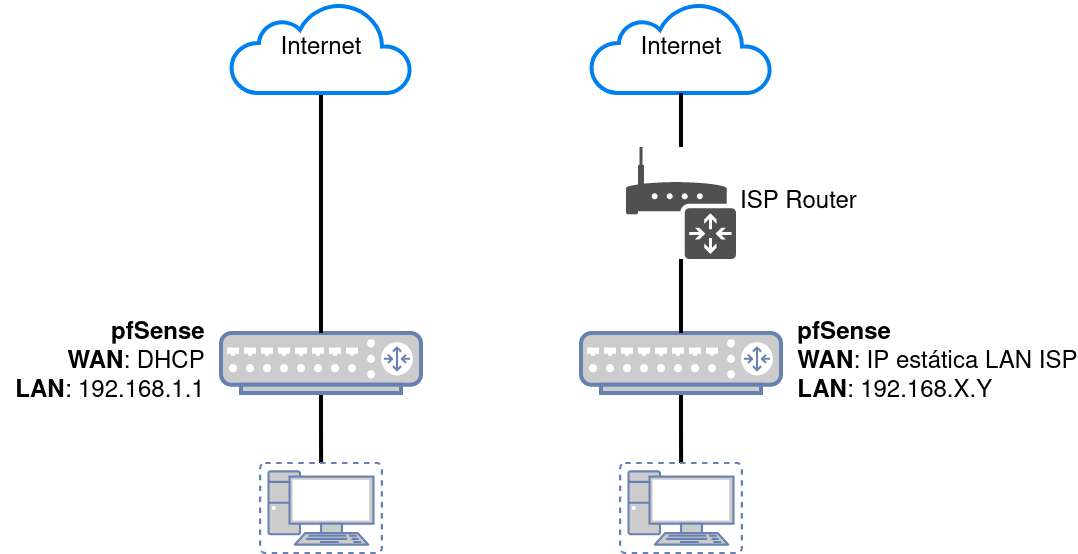
\includegraphics[width=\linewidth]{pfsense_infraestructure.png}
\end{center}


\begin{itemize}
    \item \textbf{1ª opción}: el pfSense actúa como conexión directa a internet. Para ello estará conectado a un router neutro, cable-modem, ONT  o lo habremos configurado como nuestro ISP nos indique. Por lo tanto pfSense tendrá IP pública a internet y actuará como firewall directo.
    \item \textbf{2ª opción}: haciendo doble NAT, detrás del router de nuestro proveedor de Internet. Para que todo funcione de manera correcta, en el router del proveedor deberemos hacer una redirección de puertos para que todas las conexiones vayan a la IP del servidor pfSense.
\end{itemize}

\section{Requisitos}
Esta simulación se puede realizar de dos maneras: haciendo uso de hardware o haciendo uso de máquinas virtuales. La manera más sencilla es realizarlo haciendo uso de máquinas virtuales con un virtualizador como es Virtualbox, por lo que se explicará esta modalidad.

En caso de querer realizar la instalación sobre hardware, sería necesario contar con un equipo que haga la función de servidor pfSense y que cuente con al menos 2 interfaces de red (uno para WAN y otro para LAN), así como otro PC que será el equipo de la LAN.


\chapter{PfSense}
\href{https://www.pfsense.org/}{PfSense} es una distribución de \href{https://es.wikipedia.org/wiki/FreeBSD}{FreeBSD} (no confundir con GNU/Linux, ya que FreeBSD es \href{https://es.wikipedia.org/wiki/Unix}{Unix}) que está adaptada para que actúe como un sistema de firewall, enrutador, control de tráfico, servidor DNS, DHCP, VPN, proxy y muchos servicios más.

Tal como veremos a continuación, la instalación es sencilla y la configuración de los servicios se realiza a través de un interfaz web desde el que se puede controlar las reglas de filtrado que se pueden crear, las configuraciones que se van a realizar, …
Hoy en día, la empresa que está detrás de pfSense, Netgate, vende unos sistemas appliance (hardware específico para realizar las funciones de firewall, con la distribución preinstalada), pero lo habitual suele ser que la instalación se realice sobre un sistema hardware de servidor o virtualizado.

A nivel de características técnicas lo único que se pide es un procesador basado en la arquitectura x86\_64 (Intel o AMD) de 600MHz, 512 MB de RAM y 4GB de disco duro. Lógicamente, este es el hardware mínimo recomendado, y dependiendo de la cantidad de tráfico que tenga nuestra infraestructura deberemos tener un hardware adecuado para el mismo. En la documentación oficial hacen referencia al \href{https://docs.netgate.com/pfsense/en/latest/hardware/size.html}{hardware que podamos necesitar} dependiendo del tráfico que vayamos a tener.

Dado que se va a optar por realizar la instalación en una máquina virtual, se va a necesitar un sistema de virtualización (Virtualbox) y el \href{https://www.pfsense.org/download/}{CD de instalación}. La instalación será idéntica si se realiza en hardware físico, o en otro sistema de virtualización.

\hypertarget{detalles_maquina_virtual}{}
\section{Detalles de la máquina virtual}
\begin{wrapfigure}{r}{0.27\linewidth}
    \centering
    \vspace{-20pt}
    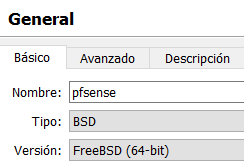
\includegraphics[frame,width=\linewidth]{vm-1.png}
\end{wrapfigure}
No se va a detallar cómo crear una máquina virtual, pero si las características técnicas que debe tener cuando se crea en Virtualbox.

Dado que pfSense está basado en un sistema Unix FreeBSD, la máquina tiene que crearse indicando el tipo “BSD” y la versión “FreeBSD” de 64 bits, tal como aparece en la imagen.

Por otro lado, a la máquina virtual se le van a añadir dos interfaces de red:

\begin{itemize}
    \item El primer adaptador de red será de tipo “Adaptador puente”, ya que en el sistema haremos que sea la interfaz que actuará como “WAN”.
    \item El segundo adaptador de red se creará de tipo “Red interna” y le pondremos el nombre de “LAN”, que hará esas funciones en nuestra infraestructura.
\end{itemize}

Dadas las explicaciones previas, una vez creada la máquina virtual nuestra infraestructura virtual quedaría de la siguiente manera:

\begin{center}
    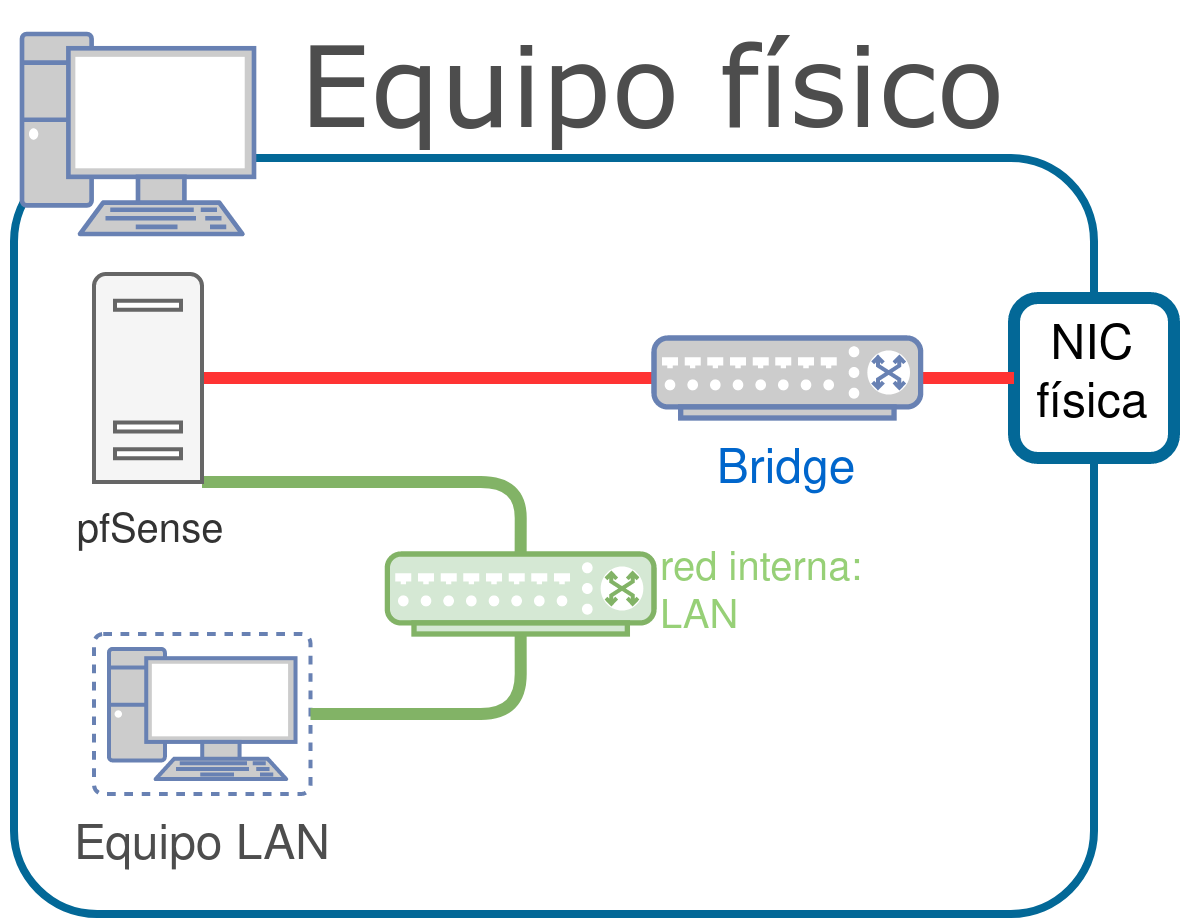
\includegraphics[width=0.5\linewidth]{infraestructura_virtualbox.png}
\end{center}

Visto este dibujo, la máquina virtual que actuará como PC dentro de la LAN le tendremos que modificar el adaptador virtual para que sea de tipo “Red interna” y escribiremos “\textbf{LAN}”, por lo que ambas máquinas estarán conectadas mediante un “switch virtual”.

El resto de parámetros de la máquina virtual, como se trata de una para pruebas, será:

\begin{itemize}
    \item 8 GB de disco duro
    \item 1GB de memoria RAM
\end{itemize}

\section{Instalación}
Tras poner el CD de instalación en la máquina virtual y arrancar veremos un pequeño menú como muestra la siguiente captura de pantalla:

\begin{center}
    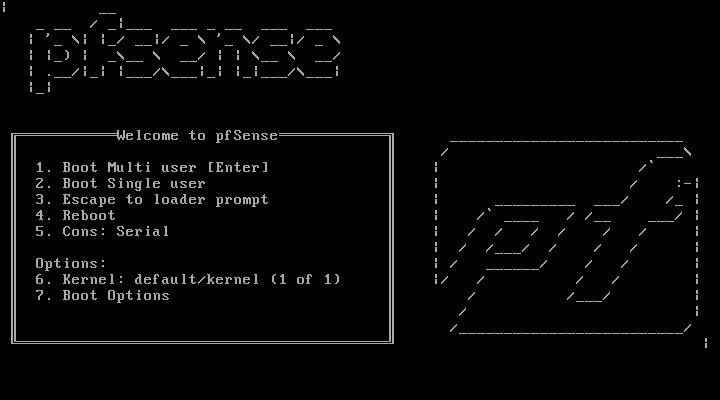
\includegraphics[width=0.7\linewidth]{install-1.png}
\end{center}

El menú contará con un sistema de cuenta atrás y si no se selecciona nada entrará en la primera opción por defecto. Se podrá ver cómo el sistema arranca y detecta el  hardware y al finalizar nos mostrará un menú con las opciones:

\begin{itemize}
    \item \textbf{Install}: Instalar pfSense
    \item \textbf{Rescue Shell}: Lanza una terminal para poder recuperar una instalación que esté dando problemas
    \item \textbf{Recover config.xml}: recupera el fichero de configuración config.xml de una instalación previa.
\end{itemize}
Tras seleccionar la opción de instalar, nos aparecerá un menú para seleccionar la distribución del teclado y a continuación el tipo de partición que queremos utilizar:

\begin{itemize}
    \item \textbf{Auto (UFS) BIOS}: si nuestro sistema usa BIOS
    \item \textbf{Auto (UFS) UEFI}: si nuestro sistema usa UEFI
    \item \textbf{Manual}: Nos permite particionar de manera manual, para expertos
    \item \textbf{Shell}: Abre una consola y podremos realizar el particionado a mano
    \item \textbf{Auto (ZFS)}: Sistema de particionado con el sistema de ficheros ZFS
\end{itemize}

Dado que nuestra máquina virtual tiene BIOS, haremos uso de la primera opción y comenzará automáticamente el particionado del disco duro. Tras terminar, nos preguntará si queremos abrir una terminal en el sistema recién instalado. Le diremos que no y que reinicie el sistema. Nos tendremos que asegurar de quitar la ISO de la máquina virtual para que arranque desde el disco duro en lugar del CD.


\chapter{Configuración básica}
En este apartado se va a detallar cómo realizar una configuración básica de pfSense para que actúe como firewall dentro de la red simulada que hemos creado.


\section{Primer arranque}
Tras realizar la instalación y reiniciar, al arrancar  desde el disco duro aparecerá un menú similar al que hemos visto al arrancar desde el CD, que si no se selecciona nada, usará la primera opción y terminará arrancando hasta llegar a otro menú.

El siguiente menú aparecerá por defecto, y en una instalación por hardware sería lo que veríamos en la pantalla tras el reinicio. Debido a que es un menú desde el que podemos realizar configuraciones es un posible fallo de seguridad el tenerlo activado, ya que un atacante con acceso al hardware (o al sistema de virtualización) podría realizar modificaciones sobre el mismo. Lo habitual suele ser deshabilitar este menú y que para poder acceder a él haya que introducir la contraseña de root.

De esta captura de pantalla del menú podemos sacar varios detalles:

\begin{center}
    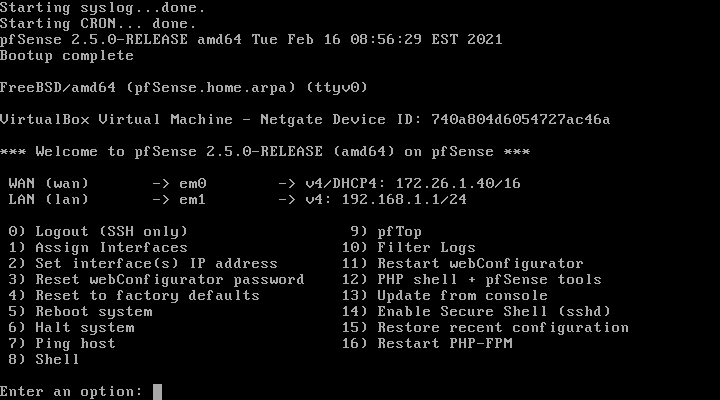
\includegraphics[width=0.7\linewidth]{boot-1.png}
\end{center}

\begin{itemize}
    \item \textbf{WAN}: Ha cogido IP por DHCP y en este caso ha obtenido la IP 172.26.1.40/16. Este será el interfaz que en una infraestructura real obtendría la IP de Internet, una IP pública.
    \item \textbf{LAN}: Automáticamente ha configurado el interfaz de la red local con la IP 192.168.1.1/24
\end{itemize}


Junto a esos nombre aparecen “em0” y “em1” que son el nombre de los interfaces “físicos” (en este caso, son interfaces de la máquina virtual). Tal como se puede ver, el primer interfaz de la máquina virtual lo ha cogido para que sea la WAN y el segundo para la LAN. Por ello, hemos tenido que realizar la configuración de los interfaces de la máquina virtual de manera correcta.


\section{Menú de configuración desde consola}
Tal como se ha comentado, el menú cuenta con distintas opciones de administración.

\begin{center}
    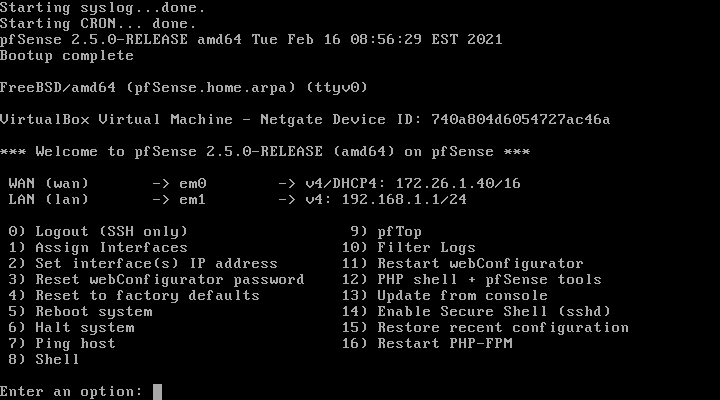
\includegraphics[trim={0 0 50 133},clip,width=0.7\linewidth]{boot-1.png}
\end{center}

Como se puede ver en la imagen previa, aparecen 16 posibles opciones a elegir, entre las que destacaremos:

\begin{enumerate}
    \item \textbf{Assign interfaces}: Para poder reconfigurar a qué red pertenecen los interfaces que tiene nuestro firewall (si es WAN, LAN, … ).
    \item \textbf{Set interfaces IP address}: Para poder modificar la IP de los interfaces que tiene nuestro firewall.
    \item \textbf{Reset webConfigurator password}: Cambiar la contraseña de acceso.
    \item \textbf{Reset to factory defaults}: Restaurar el servidor a los valores de “fábrica”, es decir, resetea todas las configuraciones propias realizadas.
    \item \textbf{Reboot}: Reinicia el servidor.
    \item \textbf{Halt}: Apaga el servidor.
    \item \textbf{Ping} host: Realiza un ping al equipo indicado.
    \item \textbf{Shell}: Nos abre una consola en el sistema para poder realizar modificaciones mediante comandos.
    \item \textbf{pfTop}: Nos muestra un listado de las conexiones establecidas en tiempo real.
    \item[14.] \textbf{Enable Secure Shell (sshd)}: Habilita el servidor SSH para poder realizar conexiones. Por defecto, sólo podremos conectarnos desde la LAN.
    \item[16.] \textbf{Restart PHP-FPM}: Reinicia el servicio del interfaz web.
\end{enumerate}

\section{Interfaz web de configuración}
El acceso a la interfaz web de configuración sólo está disponible desde la red LAN, por lo que accederemos desde la máquina virtual dentro de la LAN abriendo un navegador y apuntando a la IP por defecto de la LAN “https://192.168.1.1”. Tendremos que aceptar el certificado de seguridad (ya que es auto-firmado) y nos aparecerá la web de login.

\begin{center}
    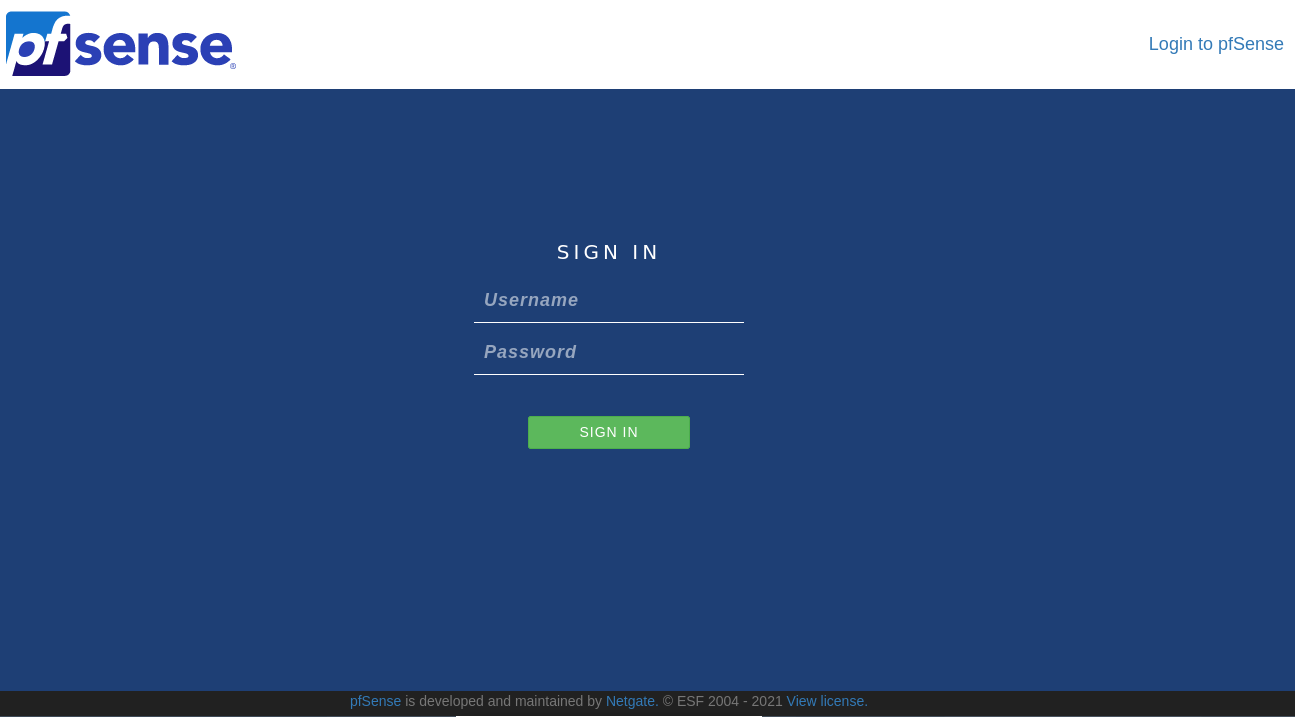
\includegraphics[frame,width=0.7\linewidth]{login.png}
\end{center}

Los credenciales por defecto son:
\begin{itemize}
    \item \textbf{username}: admin
    \item \textbf{password}: pfsense
\end{itemize}

El usuario admin de la web tendrá la misma contraseña que el usuario root por consola, por lo que tendrá que ser una contraseña segura y que sólo los administradores del servidor conozcan.

Cuando nos logueamos por primera vez nos aparecerá la primera página del asistente de configuración de pfsense, que nos guiará a través de nueve pasos donde podremos hacer una configuración básica de pfSense. Los pasos serán los siguientes:

\begin{enumerate}
    \setcounter{enumi}{0}
    \item \textbf{Bienvenida al asistente}: página de inicio
    \item \textbf{Soporte de Netgate}: detrás de pfSense hay una empresa, Netgate, que ofrece sus servicios de soporte para pfSense
    \item \textbf{Información general}: configuración básica del servidor:
    \begin{itemize}
        \item \textbf{hostname}: nombre del servidor
        \item \textbf{domain}: nombre del dominio al que pertenece el servidor
        \item \textbf{DNS Server}: servidores DNS externos al que mandar las peticiones.
    \end{itemize}
    \item \textbf{Servidor de tiempo}: configurar la zona horaria y el servidor NTP
    \item \textbf{Configurar interfaz WAN}: Dependiendo de cómo sea la infraestructura real, podremos configurar el interfaz WAN con IP pública estática, por DHCP, por PPPoE, … Por defecto está en DHCP. Si estamos tras doble NAT, habría que desactivar la opción “RFC1918 Networks”
    \item \textbf{Configurar interfaz LAN}: La IP de pfSense en el direccionamiento LAN. Por defecto es 192.168.1.1 con una máscara “/24”.
    \item \textbf{Cambio de contraseña del admin}: Para poner una contraseña más segura.
    \item \textbf{Recargar la configuración}: Si se ha realizado algún cambio, recargará la configuración
\end{enumerate}

\section{Reglas de filtrado}
PfSense es un servidor que actúa como firewall y por tanto permite la creación de reglas de filtrado de tráfico para todos los interfaces que tiene configurados. Las reglas se ejecutan cuando el tráfico \textbf{entra al interfaz} y son evaluadas en base a “primer acierto”.

Si el tráfico no coincide con alguna regla que sea explícitamente \textbf{pass} el tráfico será denegado. Por defecto pfsense deniega todo el tráfico entrante a sus interfaces. Las acciones principales de las reglas pueden ser:
Pass: Permite el tráfico al destino.

\begin{itemize}
    \item \textbf{Reject}: Rechaza el paquete y avisa al emisor.
    \item \textbf{Block}: Rechaza el paquete de manera silenciosa.
\end{itemize}

Aunque las opciones “\textit{block}” y “\textit{reject}” rechazan el paquete, la diferencia puede suponer una gran diferencia, ya que “reject” responde con \textbf{TCP RST }(o "\textit{port unreacheable}"), y eso puede permitir la posibilidad de recibir un ataque de denegación de servicio.

\errorbox{\textbf{¡Nunca se debería usar “\textit{reject}” en el interfaz  WAN!}}

En redes privadas es útil hacer uso de “\textit{reject}”, porque avisa a los programas que intentan realizar conexiones que la conexión está bloqueada, y por tanto la respuesta es más rápida ya que no se esperan timeouts.

\hypertarget{ciclo_vida_conexiones}{}
\subsection{Ciclo de vida de una conexión}
A continuación se explica cómo actúa pfSense al recibir un paquete de una nueva conexión:

\begin{itemize}
    \item El paquete, como parte de una nueva conexión, llega a un interfaz.
    \item Se comprueban las reglas de filtrado \textbf{en orden descendiente} contra el paquete.
    \item Cuando existe coincidencia, se ejecuta la acción de la regla de filtrado.
    \item Se para las comprobaciones de las reglas.
    \item Si no ha existido una coincidencia tras comprobar todas las reglas, el paquete es bloqueado por defecto.
\end{itemize}


\subsection{Reglas creadas por defecto}
Tras la instalación de PfSense podemos ir a “Firewall → Rules” y ahí aparecen los interfaces que están configurados actualmente y en los que se pueden crear reglas de filtrado. Los interfaces que existirán en nuestra infraestructura serán:

\begin{itemize}
    \item \textbf{Floating}: No es una interfaz al uso. Es para crear reglas de filtrado especiales que se pueden saltar el orden y/o aplicar a todos los interfaces. \textbf{Es mejor no utilizarlo salvo que sepamos qué estamos haciedno y hayamos leído detenidamente} la \href{https://docs.netgate.com/pfsense/en/latest/firewall/floating-rules.html}{documentación} sobre ello.
    \item \textbf{WAN}: Bloquea todos los paquetes.
    \item \textbf{LAN}: Existen varias reglas creadas por defecto que permiten tráfico:

    \begin{center}
        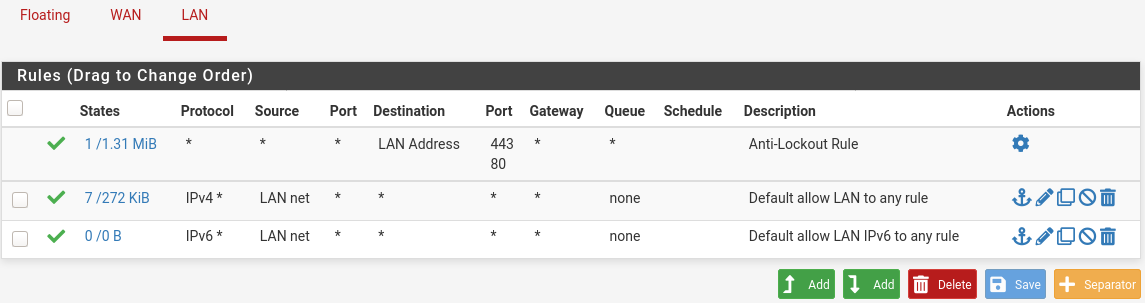
\includegraphics[frame,width=\linewidth]{firewall-1.png}
    \end{center}

    \begin{enumerate}
        \item[\faCheck] Permite el acceso a la IP de la LAN del pfsense al puerto 80 y 443 para poder administrarlo vía web. Esta regla está especialmente creada para que no se pueda eliminar desde este apartado, ya que el borrarla podría suponer no poder configurar pfSense vía web.
        \item[\faCheck] Permite cualquier tráfico de tipo IPv4
        \item[\faCheck] Permite cualquier tráfico de tipo IPv6
    \end{enumerate}
\end{itemize}

Las últimas dos reglas explicadas previamente permiten que el tráfico pueda salir de la LAN hacia internet y así se permita navegar por internet. Si se crease una nueva red LAN (para una red wifi, DMZ, …) estas reglas no estarían creadas, por lo que desde esa nueva LAN no se podría acceder a ninguna otra red, por lo que habría que crear reglas que permitieran el tráfico.

\subsection{Crear regla de denegación}
Tal como se ha comentado, actualmente desde la LAN se permite acceder a cualquier red, por lo que podemos hacer ping a cualquier equipo de internet. Como ejemplo se va a crear una regla que impedirá el acceso a un servidor de internet. Esta regla servirá de ejemplo para poder realizar cualquier otra regla que sea necesaria.

La regla se va a crear en el interfaz LAN, ya que queremos limitar el tráfico al entrar desde esta red. Para crear la regla existen dos botones de creación:

\begin{itemize}
    \item \textbf{Añadir la regla al principio de la lista}: como su propio nombre indica, creará la regla al principio de la lista en la que aparecen todas las reglas que ya están creadas.
    \item \textbf{Añadir la regla al final de la lista}: en este caso creará la lista al final de todas las reglas.
\end{itemize}

No importa dónde se cree la nueva regla, ya que se podrá modificar después su posición. Al crear la regla, tendremos que tener en cuenta los siguientes apartados:

\begin{itemize}
    \item \textbf{Action}: Qué queremos hacer con la regla: \textbf{pass}, \textbf{block} o \textbf{reject}.
    \item \textbf{Disabled}: Para deshabilitar la regla. Suele ser buena idea deshabilitar temporalmente las reglas que no se necesiten en lugar de borrarlas, por si nos hemos confundido y hay que recuperarlas.
    \item \textbf{Interface}: El interfaz sobre la que se va a crear la regla.
    \item \textbf{Familia de dirección}: Si queremos aplicar la regla sobre IPv4, IPv6 o ambas.
    \item \textbf{Protocolo}: Protocolo de la conexión: TCP, UDP, ICMP, Any…
    \item \textbf{Source}: Origen de la conexión. Si es “Any” será desde cualquier equipo de la red elegida. Podremos elegir un único equipo u otras opciones.
    \item \textbf{Destination}: El destino de la conexión. Si es “Any” será a cualquier equipo. Podremos elegir un equipo u otras opciones.
    \item \textbf{Extra options}: Opciones extra y avanzadas para la regla (limitar número de conexiones, modificar el gateway de salida, … ).
    \item \textbf{Description}: Suele ser recomendable añadir una descripción a las reglas para identificar el servicio o el servidor sobre el que se aplica.
\end{itemize}

Para el ejemplo se va a bloquear todo el tráfico desde la LAN, al servidor 1.1.1.1 (servidor DNS de la empresa Cloudflare). La regla quedaría:

\begin{center}
    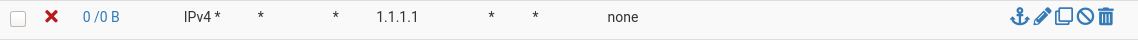
\includegraphics[trim={0 0 490 0},clip,frame,width=\linewidth]{firewall-2.png}
\end{center}


\begin{wrapfigure}{r}{0.2\linewidth}
    \centering
    \vspace{-10pt}
    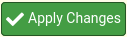
\includegraphics[width=\linewidth]{apply.png}
\end{wrapfigure}
Una vez creada la regla aparecerá un botón para aplicar los cambios, por lo que hasta que no sea pulsado ese botón, las nuevas reglas que se hayan creado no tendrán efecto y por tanto no entrarán en funcionamiento.


\subsection{Orden de las reglas}
Tal como se ha identificado en el ciclo de \hyperlink{ciclo_vida_conexiones}{vida de las conexiones}, el orden de las reglas es muy importante, ya que en el momento en el que el tráfico entra sobre el interfaz se comprobará si coincide con las reglas en orden descendente.

Por lo tanto, si existe una regla muy general que permite el tráfico y después una muy específica de bloqueo, es bastante probable que la regla específica de bloqueo no llegue a entrar en funcionamiento, ya que el tráfico coincidirá con la regla general que permite dicho tráfico.

Teniendo en cuenta la regla creada en el apartado anterior, vamos a analizar cuál es el comportamiento dependiendo del orden en el que se sitúa:

\begin{itemize}
    \item Al \textbf{final} del todo:
    \begin{center}
        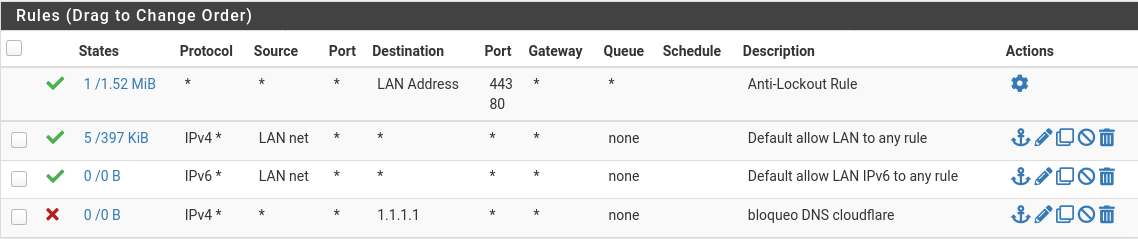
\includegraphics[frame,width=\linewidth]{firewall-3.png}
    \end{center}
    Teniendo en cuenta las reglas creadas sobre el interfaz LAN en este orden, la regla de bloqueo al servidor 1.1.1.1 no entrará nunca en funcionamiento. El tráfico cuyo origen sea la LAN coincidirá siempre con la regla que le permite ir a cualquier parte, por lo que al coincidir con esa regla no se analizará ninguna más.

    \item Al \textbf{comienzo} de las reglas:
    \begin{center}
        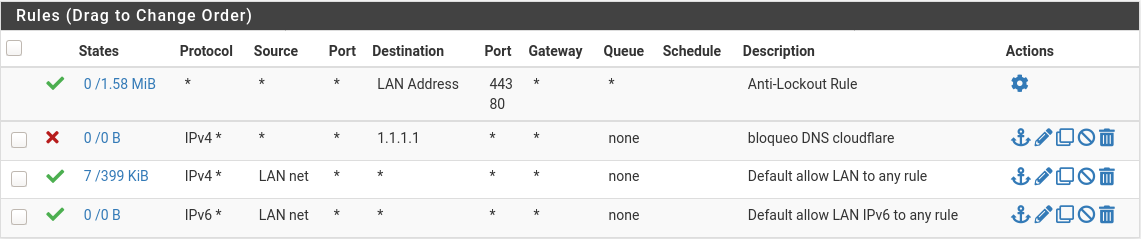
\includegraphics[frame,width=\linewidth]{firewall-4.png}
    \end{center}
    En este caso la regla más específica de denegación se ha puesto al principio, por lo que si el tráfico coincide con esta hará lo que indica la regla, bloquear el tráfico al servidor 1.1.1.1. Si no coincide, se seguirán analizando el resto de reglas, y en este caso se permitirá el resto de tráfico.
\end{itemize}

Es de vital importancia tener en cuenta el orden de las reglas, analizarlo con cuidado y realizar las pruebas oportunas para confirmar que lo que se pretende hacer es lo que termina sucediendo.

\errorbox{\textbf{¡El orden de las reglas de filtrado es muy importante en cualquier Firewall!}}


\chapter{Crear una nueva red}
Teniendo en cuenta lo visto hasta ahora, nuestra infraestructura cuenta con una única red LAN detrás del firewall y, aparte, el acceso a WAN. En este apartado se va a explicar cómo crear una nueva red para una sección DMZ (\href{https://es.wikipedia.org/wiki/Zona_desmilitarizada_(inform%C3%A1tica)}{zona desmilitarizada}) en la que se instalarán servidores.
Normalmente lo habitual suele ser que el acceso desde y hasta la DMZ cumpla con las siguientes restricciones:

\begin{itemize}
    \item \textbf{LAN → DMZ: permitido/limitado}, para el acceso a servicios como carpetas compartidas, páginas web, … Se permitirá sólo a los servicios que se ofrecen.
    \item  \textbf{DMZ → LAN}: bloqueado. El acceso desde la DMZ a la LAN suele estar bloqueado ya que los servidores no deberían poder acceder a los equipos de los usuarios.
    \item \textbf{DMZ → Internet}: limitado. Dependerá de los servicios que estén instalados en los servidores. Para el acceso total a internet (para actualizaciones de software, por ejemplo) se suele permitir el acceso a través de un proxy que realizará el bloqueo y sólo permitirá las webs correspondientes.
    \item \textbf{Internet → DMZ}: limitado. Dependerá de los servicios que estén instalados en los servidores. Sólo se permitirá el acceso a los puertos de los servicios necesarios.
\end{itemize}

\section{Modificando la infraestructura creada}
Dado que se va a crear una red nueva, deberemos realizar cambios en la máquina virtual de nuestro servidor pfSense. La nueva infraestructura será la siguiente:

\begin{center}
    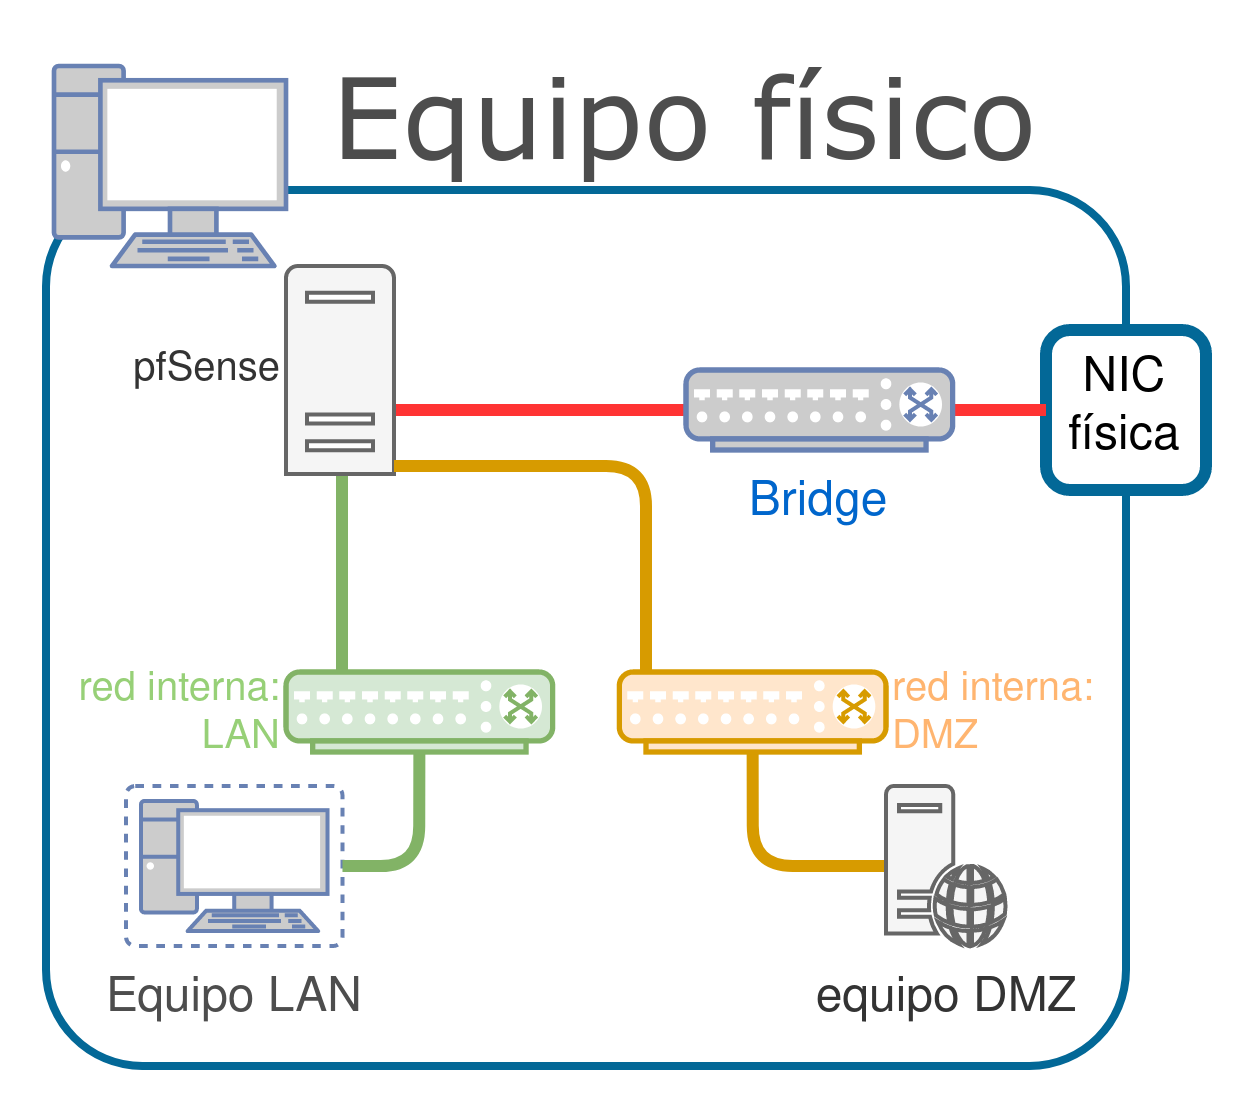
\includegraphics[width=0.5\linewidth]{infraestructura_dmz_virtualbox.png}
\end{center}

Tal como se puede apreciar al compararlo con la \hyperlink{detalles_maquina_virtual}{infraestructura anterior}, se ha creado una nueva red interna, por lo que al pfSense se le tendrá que activar una nueva interfaz de tipo “Red interna” y le daremos el nombre de DMZ.

Virtualbox no nos permite realizar esta modificación “en caliente”, por lo que habrá que apagar la máquina virtual de pfSense. Algunos sistemas profesionales de virtualización sí que permiten hacer algunas modificaciones hardware en las máquinas virtuales sin tener que apagarlas, y dependiendo del sistema operativo, se dará cuenta de dichos cambios y por lo tanto no será necesario realizar un apagado.

Crearemos otra máquina virtual que actuará a modo de servidor en la red DMZ, por lo que en su configuración la configuraremos también como “Red interna” en DMZ.


\section{Modificación de la configuración en pfSense}
Tal como se ha visto, tras la instalación de pfSense aparece un pequeño asistente de configuración que nos lleva a través de unos pasos que nos permitirá realizar la configuración de una infraestructura basada en una red con parte WAN y LAN.

En caso de tener más interfaces de red durante la instalación, o a posteriori como sucede ahora, no se configurarán y por tanto queda en nuestra mano realizar dicha configuración.


\subsection{Añadir y configurar interfaz}
Dado que pfSense cuenta con un nuevo interfaz, por defecto aparece deshabilitado y sin configurar. Debemos activarlo, darle el direccionamiento que veamos adecuado y lo habitual también suele ser darle un nombre representativo de la red que va a servir.

Todas estas modificaciones se realizan desde el interfaz web, a través de “\textit{\textbf{Interfaces → Assignments}}”:

\begin{center}
    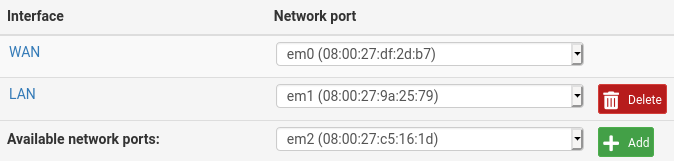
\includegraphics[frame,width=0.8\linewidth]{interfaces.png}
\end{center}

Tal como se puede ver, aparece la nueva interfaz junto a un botón “Add” que indica que lo podemos añadir a la configuración. Una vez pulsado el botón se le asigna el nombre “OPT1” como nombre por defecto, pero la idea es cambiarlo. Para ello se hace click en el interfaz, y se entra en su configuración.

Entre las modificaciones que vamos a realizar están:

\begin{itemize}
    \item \textbf{Enable}: hay que habilitar el interfaz, ya que aunque esté configurado, si no está habilitado no entrará en funcionamiento.
    \item \textbf{Description}: El nombre que le daremos al interfaz, en este caso “DMZ”.
    \item \textbf{IPv4 Configuration Type}: Tipo de IPv4 que se le va a asignar. Crearemos un direcconamiento estático, por ejemplo: 172.16.0.1 /25 . La configuración de la red se hace en la misma página, un poco más abajo.
\end{itemize}

Una vez realizados los cambios, habrá que aplicar los cambios.


\subsection{Configurar DHCP Server}
Aunque no suele ser habitual configurar el DHCP Server en la red DMZ, se va a explicar cómo realizar la configuración ya que en otro tipo de redes (para el WIFI, departamento de marketing, … ) es útil.

Para realizar la configuración se hace en “\textbf{\textit{Services → DHCP Server}}”, donde aparecerán las interfaces sobre las que podemos gestionar dicho servicio, actualmente en LAN y DMZ.

La configuración que se tendrá en cuenta a la hora de modificar el DHCP en el interfaz será:

\begin{itemize}
    \item \textbf{Enable}: Habilitar servicio
    \item \textbf{Range}: Si queremos limitar el DHCP para que sólo de IPs a una parte de la red
    \item \textbf{Other Options}: Los servidores DHCP no sólo se encargan de dar IPs, por lo que hay muchas opciones extra que se pueden modificar
\end{itemize}

\subsubsection{Mapear IPs de DHCP a estática}
Existe la posibilidad de dar a los equipos siempre la misma IP cuando hacen una petición DHCP. Los servidores DHCP suelen crear una pequeña base de datos con las IPs que han otorgado y durante cuánto tiempo las tienen reservadas para esos equipos.

Es posible realizar mapeos de IPs a equipos que sean permanentes, por lo que los equipos que pidan DHCP, si tienen dicho mapeo creado, siempre se les asignará la misma IP y esa IP estará reservada sólo para ese equipo.

Suele ser habitual el realizar estos mapeos para tener controlados los equipos y conocer sus IPs sin tener que ir a ellos a configurarlos de manera estática, ya que todo se queda centralizado en el servidor DHCP.

Para realizar estos mapeos hay que ir a “Status → DHCP Leases” donde podremos ver todas las IPs que se han otorgado:

\begin{center}
    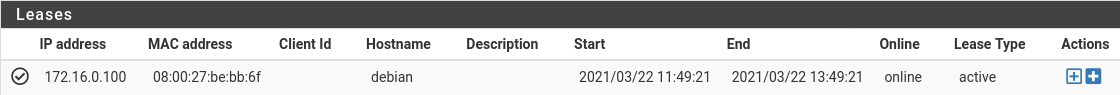
\includegraphics[frame,width=0.9\linewidth]{dhcp_lease.png}
\end{center}

\subsection{Modificación de reglas de filtrado}

    \part{Anexos}
    \graphicspath{{../../../anexos/instalar_ubuntu_lts/img/}}
    \hypertarget{instalar_ubuntu_lts}{}

\chapter{Instalar Ubuntu 20.04 LTS}
En este anexo realizaremos la instalación de la distribución Ubuntu 20.04 LTS en su versión para servidores. En este anexo no se va a explicar cómo realizar la creación de una máquina virtual donde se aloja el sistema operativo, ya que existen distintos tipos de virtualizadores.

No se realizará una guía “paso a paso”, sino que se centrará en las partes más importantes de la instalación y en las que más dudas puedan surgir.

\section{Descargar Ubuntu 20.04}
La ISO la obtendremos de la \href{https://ubuntu.com/#download}{web oficial} y seleccionaremos la versión 20.04 LTS de Ubuntu Server. Esta ISO contendrá el sistema base de Ubuntu y nos guiará para realizar la instalación del sistema operativo.

Una vez descargada la ISO tendremos que cargarla en el sistema de virtualización elegido y arrancar la máquina virtual.


\section{Instalar Ubuntu 20.04}
Tras arrancar la máquina virtual nos aparecerá un menú para seleccionar el idioma durante la instalación y le daremos a “Instalar Ubuntu Server”.

\begin{center}
    \vspace{-10pt}
    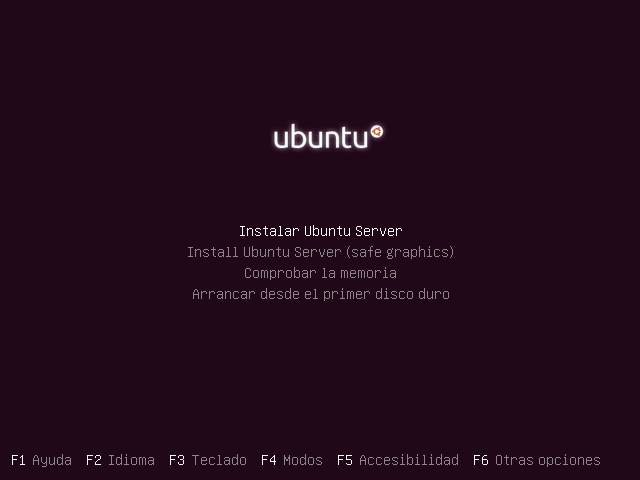
\includegraphics[width=15cm]{ubuntu_1.png}
    \vspace{-20pt}
\end{center}

A partir de aquí comenzará el instalador y los pasos que nos aparecerán serán los siguientes (algunos de estos pasos puede que no estén 100\% traducidos al castellano):

\begin{enumerate}
    \item Elegir el idioma del sistema
    \item Actualización del instalador:
    \begin{itemize}
        \item Si la máquina virtual se puede conectar a internet, comprobará si existe una actualización del propio instalador de Ubuntu.
        \item Podemos darle a “Continuar sin actualizar”
    \end{itemize}
    \item Configuración del idioma del teclado
    \item Configuración de la red
    \item Configuración del proxy de red
    \item Configuración del “mirror” o servidor espejo desde donde descargarse los \hyperlink{paquete_de_software}{paquetes de software} para las actualizaciones posteriores.
    \item Selección del disco duro donde realizar la instalación
    \item Elegir el particionado de disco.
    \item Configuración del perfil. Introduciremos el nombre de usuario, el nombre del servidor y la contraseña del usuario que vamos a crear.
    \item Configuración de SSH Server. Aceptaremos que se instale el servidor SSH durante la instalación. En caso de no seleccionar esta opción, posteriormente podremos realizar la instalación.
    \item “Featured Server Snaps”. En esta pantalla nos permite instalar software muy popular en servidores.
\end{enumerate}


Una vez le demos a continuar, comenzará la instalación en el disco duro. Debido a que durante la instalación tenemos conexión a internet, el propio instalador se descarga las últimas versiones de los paquetes de software desde los repositorios oficiales.


Al terminar la instalación, tendremos que reiniciar la máquina virtual.

\section{Post-instalación}
Tras realizar el reinicio de la máquina virtual nos encontraremos con que el sistema arranca en el sistema recién instalado, y que tendremos que loguearnos introduciendo el usuario y la contraseña utilizadas en la instalación.

\subsection{Actualización del sistema}
Por si acaso, realizaremos la actualización del índice del repositorio, actualizaremos el sistema y en caso necesario realizaremos un nuevo reinicio:

\begin{mycode}{Actualizar Ubuntu}{console}{}
mikeldi@ubuntu:~$ sudo su
[sudo] password for mikeldi:
root@ubuntu:~# apt update
...
root@ubuntu:~# apt upgrade
...
\end{mycode}

Con estos comandos nos aseguramos que el sistema está actualizado a los últimos paquetes que están en el repositorio.


\hypertarget{configurar_ip_estatica_ubuntu}{}
\subsection{Poner IP estática}
Debido a la configuración de red de nuestro servidor, la IP está puesta en modo dinámica, esto quiere decir que nuestro equipo ha cogido la IP por configuración de DHCP de nuestra red. Debido a que un servidor debe de tener IP estática, tenemos que realizar la modificación adecuada para ponerle la IP estática que mejor nos convenga. Para ello editaremos el fichero de configuración situado en la siguiente ruta: \configfile{ /etc/netplan/00-installer-config.yaml }

Lo modificaremos para que sea parecido a (siempre teniendo en cuenta la IP y gateway de nuestra red):


\begin{mycode}{Configurando IP estática en Ubuntu}{yaml}{}
network:
  ethernets:
    enp1s0:
      dhcp4: false
      addresses: [192.168.1.199/24]
      routes:
      - to: default
        via: 192.168.1.1
      nameservers:
        addresses: [8.8.8.8,1.1.1.1]
  version: 2
\end{mycode}

El fichero de configuración que hemos modificado es de tipo \href{https://es.wikipedia.org/wiki/YAML}{YAML}, que es un formato de texto que suele ser utilizado en programación o en ficheros de configuración. Este tipo de ficheros tiene en cuenta los espacios para el uso de la identación, y no suele permitir el uso de tabuladores.

Para aplicar los cambios realizados en el fichero de configuración deberemos ejecutar el siguiente comando que aplicará los cambios:

\begin{mycode}{Aplicar configuración de IP}{console}{}
root@ubuntu:~# netplan apply
\end{mycode}

\clearpage

    \graphicspath{{../../../anexos/virtualbox_networking/img}}
    \chapter{Virtualbox y adaptadores de red}

\section{Introducción}
\href{https://www.virtualbox.org/}{Virtualbox} es una herramienta de virtualización para crear máquinas virtuales de manera sencilla. Es multiplataforma por lo que se puede utilizar en Windows, MacOS y Linux y aparte, es \hyperlink{software_libre}{Software Libre}.

Este documento no va a entrar en detalle en cómo se crean las máquinas virtuales, sino que va a explicar los distintos modos y adaptadores de red que puede tener una máquina virtual en este sistema de virtualización.

\section{Adaptadores de red}
Virtualbox permite que cada máquina virtual cuente con hasta cuatro adaptadores de red, lo que comúnmente se llaman interfaces o NIC (network interface controller).

Al crear las máquinas virtuales sólo tienen un único adaptador activo y suele estar configurado en modo NAT, pero tal como se ve a continuación, en el desplegable se puede ver que existen otras opciones:

\begin{center}
    \vspace{-10pt}
    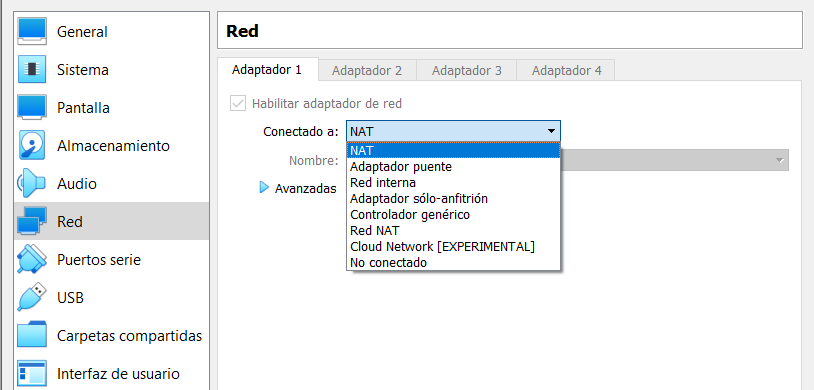
\includegraphics[frame,width=0.7\linewidth]{virtualbox_1.png}
    \vspace{-20pt}
\end{center}

En la \href{https://www.virtualbox.org/manual/ch06.html}{documentación oficial} aparece la explicación de los distintos modos, y es buena práctica leer y entender la documentación del software que utilizamos. También hay que entender que cada tipo de adaptador contará con una serie de ventajas y una serie de limitaciones que aparecen reflejadas en la documentación. Estos modos son comunes a otros  sistemas de virtualización (VmWare, Proxmox, …), pero el nombre o el modo de uso puede variar así como las posibles limitaciones que puedan existir.

A continuación se va a dar una pequeña introducción a cada tipo de adaptador.

\subsection{Adaptador puente}
Es el tipo de adaptador que se usará si queremos que las máquinas virtuales aparezcan en la red física como si fueran un equipo más. Para poder entenderlo de mejor manera, podríamos pensar que este tipo de adaptador lo que hace es crear un “switch virtual” entre las máquinas virtuales y el interfaz físico, por lo que es como si fueran un equipo más en la red física.

Si el equipo físico anfitrión cuenta con más de un NIC (por ejemplo, en un portátil el NIC por cable y el NIC wifi) tendremos que elegir en la máquina virtual sobre qué NIC queremos hacer el puente. En la siguiente imagen en el desplegable sólo se puede seleccionar un interfaz porque el equipo sólo cuenta con un NIC físico.

\begin{center}
    \vspace{-10pt}
    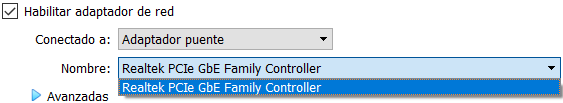
\includegraphics[frame,width=0.7\linewidth]{virtualbox_2.png}
    \vspace{-20pt}
\end{center}

Es el método utilizado cuando virtualizamos servidores, ya que podrán dar sus servicios a toda la red.

\begin{center}
    \vspace{-10pt}
    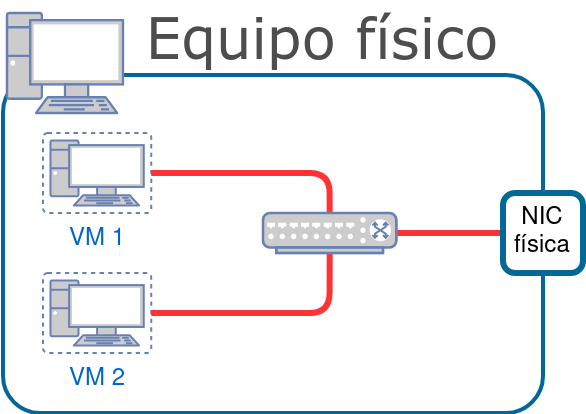
\includegraphics[width=7cm]{virtualbox-bridge.png}
    \vspace{-10pt}\captionof{figure}{Red como Adaptador Puente}
    \vspace{-20pt}
\end{center}

\subsection{NAT}
Cada máquina virtual contará con su propio “router virtual” que hará NAT, y por eso todas las máquinas virtuales que usen este modo suelen tener la misma IP, pero no pertenecen a la misma red.
Por defecto no se puede realizar conexión desde la red física al equipo virtualizado.

\begin{center}
    \vspace{-10pt}
    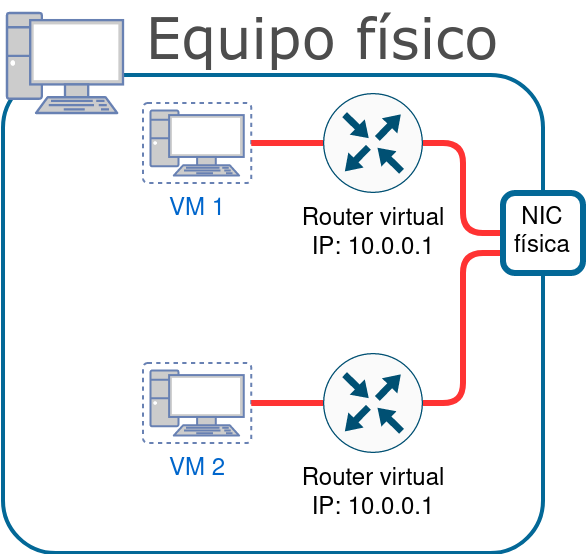
\includegraphics[width=7cm]{virtualbox-NAT.png}
    \vspace{-10pt}\captionof{figure}{Red en modo NAT}
    \vspace{-20pt}
\end{center}

\subsection{Red interna}
Este tipo de adaptador lo que hace es “crear” un “switch virtual” que unirá las distintas máquinas virtuales que estén conectadas al nombre de esa red interna.

En el siguiente ejemplo la VM1 tiene 2 NICs, cada una con una red interna distinta. La VM2 tiene un NIC conectado a una de las redes internas creadas previamente y VM3 está conectada a la otra red interna.

Virtualbox no se encarga de dar IPs en estas redes, por lo que deberemos configurar cada interfaz de la máquina virtual con el direccionamiento que nos interese.

Este método se utiliza si queremos comunicar máquinas virtuales entre sí y que estén aisladas, ya que no podrán conectarse con el exterior, ni siquiera con el propio equipo físico.

\begin{center}
    \vspace{-10pt}
    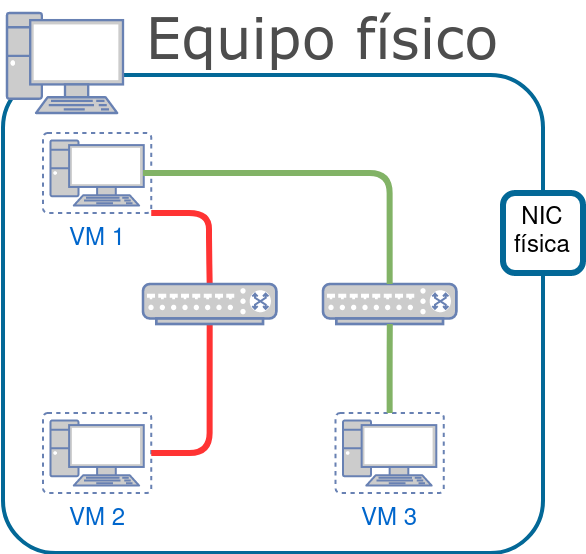
\includegraphics[width=7cm]{virtualbox-red_interna.png}
    \vspace{-10pt}\captionof{figure}{Red Interna}
    \vspace{-20pt}
\end{center}

\subsection{Red NAT}
Podría definirse como una mezcla de NAT y red interna. Las máquinas virtuales podrán pertenecer a una única red, se podrán comunicar entre ellas, estarán detrás de un NAT de la red física y se podrán comunicar con el exterior.

Para poder usar ese modo hay que crear la “red NAT” en Virtualbox yendo a “\textit{Archivo → Preferencias → Red}” y ahí se creará las redes NAT que queramos con el direccionamiento interno que nos interese.

\begin{center}
    \vspace{-10pt}
    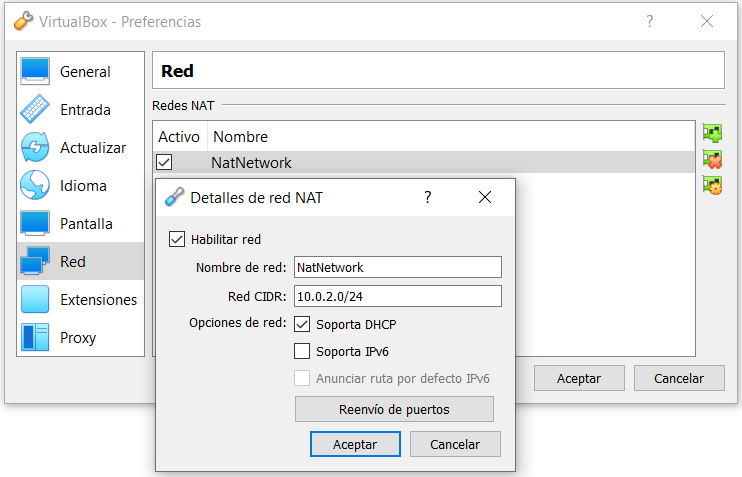
\includegraphics[width=8cm]{virtualbox-red-NAT_config.png}
    \vspace{-20pt}
\end{center}

A la hora de crear la máquina virtual y elegir la opción “Red NAT” se podrá elegir entre las redes creadas en el paso anterior.

\begin{center}
    \vspace{-10pt}
    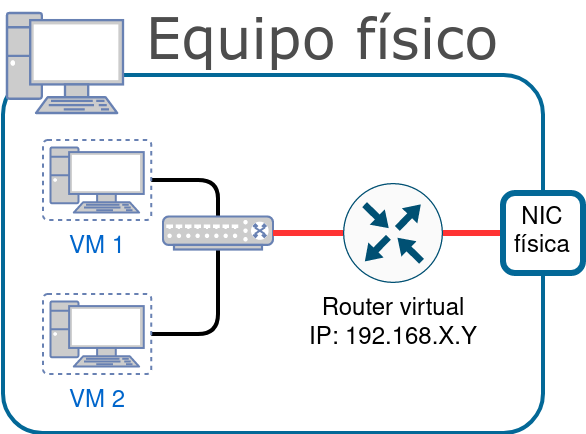
\includegraphics[width=7cm]{virtualbox-red-NAT.png}
    \vspace{-10pt}\captionof{figure}{Red NAT}
    \vspace{-20pt}
\end{center}

\subsection{Adaptador sólo-anfitrión}
Este tipo de adaptador es similar al de “red interna” pero con la posibilidad de comunicarse con el equipo físico anfitrión. En el equipo físico se crea un interfaz virtual y a través de él se podrá comunicar con las máquinas virtuales.

\begin{center}
    \vspace{-10pt}
    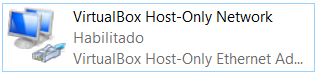
\includegraphics[width=7cm]{virtualbox-host_only_nic.png}
    \vspace{-20pt}
\end{center}

El direccionamiento que existe entre las VMs y el host se define en Virtualbox, dentro de “\textit{Archivo → \textbf{Administrador de red de anfitrión}}”. Las máquinas virtuales podrán coger IP de ese direccionamiento  por DHCP.

Mismo uso que “red interna” pero añadiendo la opción de comunicarnos con el host anfitrión.

\begin{center}
    \vspace{-10pt}
    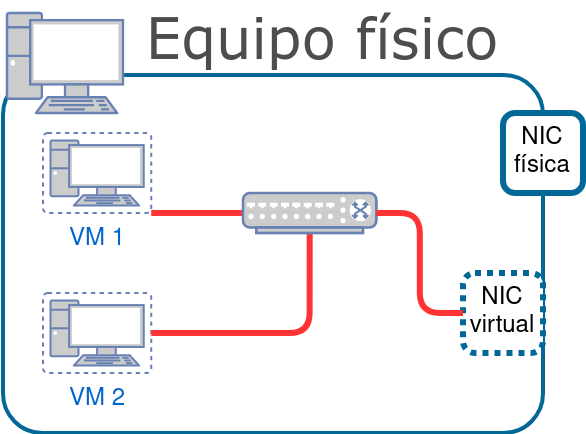
\includegraphics[width=7cm]{virtualbox-host_only.png}
    \vspace{-10pt}\captionof{figure}{Red en modo “Sólo Anfitrión”}
    \vspace{-20pt}
\end{center}

\section{Resumen de los adaptadores}
A continuación se expone una tabla que resume los distintos tipos de adaptadores que existen y la conectividad posible entre las máquinas virtuales que usan esos adaptadores y el host anfitrión (\href{https://www.virtualbox.org/manual/ch06.html#networkingmodes}{fuente}).

\begin{center}
    \vspace{-10pt}
    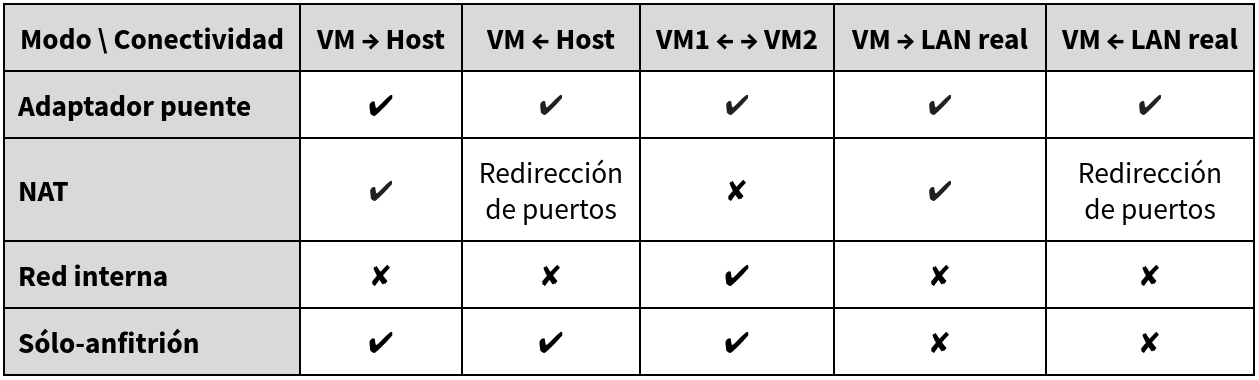
\includegraphics[width=\linewidth]{virtualbox_tabla.png}
    \vspace{-20pt}
\end{center}

En la \href{https://www.virtualbox.org/manual/ch06.html#natforward}{documentación} se explica cómo realizar la redirección de puertos.


\clearpage
    %
    \graphicspath{{../../../anexos/}}
    \chapter{Glosario}

A continuación se expone un glosario de términos con sus correspondientes definiciones:

\begin{description}
    \hypertarget{altadisponibilidad}{}
    \item[Alta Disponibilidad:] Es un diseño de arquitectura de sistemas y la implementación que asegura que el servicio instalado y otorgado sea funcional sin que haya parada en el mismo. Esta arquitectura trata de que no haya ningún \hyperlink{spf}{\textit{single point of failure} (punto único de fallo)} en la misma.

    \hypertarget{cluster}{}
    \item[Clúster:] Se denomina clúster a un conjunto de ordenadores unidos entre sí mediante conectividad de red que actúan como si de un único servidor se tratara. Dependiendo del tipo de clúster que se va a crear, debe de ser pensado desde el diseño del servicio, ya que es la aplicación o servicio quién se encarga de crear el clúster (como ocurre con MySQL Cluster).

    \hypertarget{dependencia_software}{}
    \item [Dependencia de software:] Cuando se crea cualquier tipo de software lo habitual es hacer uso de otro software (librerías de seguridad, acceso a disco, codecs de vídeo, librerías 3D…) que son necesarias para el correcto funcionamiento de nuestro programa. Este otro software (que puede ser propio o ajeno) se denomina \textbf{dependencia}, ya que sin él, nuestro programa no funcionará y es necesario que exista en el sistema para hacer funciona nuestro programa.

    En las \hyperlink{distribucion_gnu_linux}{distribuciones GNU/Linux} se hace uso de los denominados \hyperlink{paquete_de_software}{paquetes de software} en los cuales se indican las dependencias que necesitan para funcionar y que por tanto se instalarán a la par que el programa elegido, por lo que nos aseguramos que el software instalado funcionará en cuanto termine la instalación.

    En caso de descargar un software ajeno de los \hyperlink{repositorio_de_software}{repositorios} oficiales de la distribución, es posible que necesitemos completar esas dependencias por nuestra cuenta, pero hoy en día es habitual que los creadores de software lo tengan en cuenta y esas dependencias estén en los repositorios oficiales.

    \hypertarget{distribucion_gnu_linux}{}
    \item [Distribución GNU/Linux:] Es una distribución de software basada en el núcleo Linux que incluye software \hyperlink{gnu}{GNU} para componer un Sistema Operativo que pueda ser utilizado por los usuarios. Cada distribución suele \hyperlink{paquete_de_software}{empaquetar el software} en un formato propio que aparte del propio software indica las \hyperlink{dependencia_de_software}{dependencias} de software que necesita para funcionar, por lo que hace que la instalación del software se realice de manera sencilla. El software de la distribución está almacenado en los \hyperlink{repositorio_de_software}{repositorios de software} oficiales de la distribución.

    Las distribuciones suelen estar orientadas para un uso generalizado, pero es cierto que algunas, por su historia o por su manera de entender el empaquetado de software, se necesitan más conocimientos, pero hoy en día no es lo habitual.

    Existen muchas distribuciones GNU/Linux, pero las que podríamos destacar son \hyperlink{ubuntu}{Ubuntu}, Debian, Red Hat y CentOS, que son las de mayor uso hoy en día a nivel profesional.

    \hypertarget{escalado_horizontal}{}
    \item[Escalado Horizontal:] Se llama escalado horizontal a la infraestructura que crece de manera horizontal añadiendo más servidores del mismo servicio. Estos servidores serán accesibles mediante un proxy o de manera directa, y todos contarán con el mismo servicio (web, base de datos, …). No confundir con un clúster, ya que la relación de los servidores en el escalado horizontal no tienen por qué ir en clúster.

    \hypertarget{escalado_vertical}{}
    \item[Escalado Vertical:] Es el incremento de hardware de un servidor. Supongamos que un servidor empieza a tener problemas de carga, pues con el escalado vertical se le añadiría más RAM, más procesador y/o discos duros más rápidos (en caso de ser una máquina virtual sería sencillo, en caso contrario habría que realizar la migración a un servidor nuevo).

    \hypertarget{gnu}{}
    \item[GNU:] Del acrónimo \textbf{GNU’s Not Unix} (GNU no es Unix) es un sistema operativo y un conjunto de programas libres cuyo origen surgió de la idea de crear un sistema operativo Unix basado en \hyperlink{software_libre}{Software Libre}.

    El desarrollo de GNU nació en 1983 por Richard Stallman comenzando por el compilador GCC, al que se fueron uniendo todo tipo de software y creando la Free Software Foundation (o FSF, fundación por el software libre) la cual creó la \hyperlink{licencias_libres}{licencia libre} más conocida actualmente: la \textbf{GPL} (GNU General Public License).

    El proyecto GNU avanzó en el tiempo y creó el kernel Hurd, pero bien es cierto que nunca llegó a ser funcional del todo y actualmente el kernel más utilizado es Linux, pero no es el único, ya que el software GNU también es usado en conjunto con otros kernels como son los \textbf{*BSD}, de ahí la importancia que cuando hacemos referencia al sistema operativo se haga uso de \hyperlink{gnu_linux}{GNU/Linux}.

    \hypertarget{gnu_linux}{}

    \itemimage{GNU/Linux:}{r}{0.21}
    {img/Gnulinux.svg.png}
    {\href{https://es.wikipedia.org/wiki/GNU/Linux\#/media/Archivo:Gnulinux.svg}{GNU/Linux: Wikipedia}}
    {
        Aunque comúnmente solemos llamar a las \hyperlink{distribucion_gnu_linux}{distribuciones} como “Linux” esto no suele ser correcto ya que en la distribución aparte del kernel va un conjunto enorme de software del proyecto GNU. Por lo tanto, lo ideal siempre es hacer uso del nombre completo GNU/Linux.

        El proyecto \hyperlink{gnu}{GNU} y sus herramientas y software son usados con otros kernels como son los *BSD en distribuciones como FreeBSD u OpenBSD. También existen versiones con kernel BSD para la distribución Debian, por lo que en ese caso sería “Debian GNU/BSD”.
    }


    \hypertarget{json}{}
    \item[JSON:] Es un formato de texto sencillo para el intercambio de datos. Aunque originalmente fue creado como notación de objetos para Javascript, su amplia utilización ha hecho que sea utilizado como alternativa a XML.


    \hypertarget{licencias_libres}{}
    \item[Licencias libres:] Una licencia de software es un contrato entre el creador (o el titular de los derechos de autor) del software y el usuario. Todo software que usamos suele exigir la lectura de esta licencia y es por ello muy importante conocer qué se puede y no se puede hacer con dicho software.

    Las licencias libres son aquellas que nos permiten hacer con el software lo que las cuatro libertades del \hyperlink{software_libre}{Software Libre} exige.

    Entre las licencias libres más utilizadas hoy en día están la GPL (General Public License del proyecto \hyperlink{gnu}{GNU}), la Apache License, algunas de las versiones de las licencias Creative Commons, …


    \hypertarget{linux}{}
    \item[Linux:] Creado originalmente por Linus Torvalds en 1991 y actualmente desarrollado por cientos de desarrolladores de todo el mundo, Linux es el núcleo (o kernel) gratuito y libre similar al núcleo de los sistemas operativos Unix.

    Comenzó como un proyecto personal de Linus (siendo estudiante universitario) para su ordenador 386 y actualmente está portado a \href{https://es.wikipedia.org/wiki/Portabilidad\_del\_n\%C3\%BAcleo\_Linux\_y\_arquitecturas\_soportadas}{decenas de plataformas hardware}. Es el proyecto más grande y ambicioso del \hyperlink{software_libre}{Software Libre}, aunque originalmente no se permitía el uso comercial del mismo (hasta la versión 0.12).

    Al poco tiempo de comenzar su desarrollo el proyecto \hyperlink{gnu}{GNU} lo adoptó como su kernel naciendo lo que actualmente conocemos como \hyperlink{gnu_linux}{GNU/Linux} y con ello cientos de \hyperlink{distribucion_gnu_linux}{distribuciones}.

    Es un núcleo de tipo monolítico que permite la carga de módulos en tiempo de ejecución


    \hypertarget{lts}{}
    \item[LTS:] Del inglés \textit{\textbf{L}ong \textbf{T}erm \textbf{S}upport} (en castellano “soporte a largo plazo”), es una característica en informática que hace referencia a versiones especiales de software que contarán con un soporte más largo del habitual, por lo que serán las versiones idóneas para usar en servidores.

    Estas versiones suelen contar con actualizaciones de seguridad, pero no con cambios notorios en la forma del software para fomentar la fiabilidad del mismo. Lo habitual es utilizar este tipo de versiones en servidores, que aunque puedan no tener las últimas modificaciones de las versiones más recientes del software, nos aseguramos la fiabilidad. Esto hace que tengamos que decidir si es necesario contar con las características de las últimas versiones (ya sea nuevos servicios, opciones nuevas, velocidad, … ) o si preferimos contar con una versión que tendrá un ciclo de vida más longevo pero con actualizaciones de seguridad.

    Es habitual verlo en proyectos de \hyperlink{software_libre}{Software Libre}, como ejemplos podemos tomar el kernel \hyperlink{linux}{Linux} (actualmente la versión 5.4.58 es la denominada LTS) y la distribución \hyperlink{ubuntu}{Ubuntu} (en este caso la versión 20.04).


    \hypertarget{paquete_de_software}{}
    \item[Paquetes de Software:] Un paquete de software no es más que una manera de poder distribuir el software creado. En \hyperlink{distribucion_gnu_linux}{distribuciones GNU/Linux} estos paquetes determinan las \hyperlink{dependencia_software}{dependencias} que necesitan para que su instalación sea lo más sencilla posible.

    Lo habitual es que estos paquetes estén gestionados mediante un sistema de gestión propio para conocer cuáles están instalados, sus dependencias, desinstalarlos de manera sencila...

    No sólo se usa en distribuciones GNU/Linux, ya que varios lenguajes de programación hacen lo propio para distribuir software en forma de paquetes. Como ejemplos:
    \begin{itemize}
        \item En distribuciones GNU/Linux tenemos APT, Yum, Zypper, Portage, ...
        \item En lenguajes de programación tenemos Gem para Ruby, Eggs para Python, CPAN en Perl, ...
    \end{itemize}


    \hypertarget{repositorio_de_software}{}
    \item[Repositorio de Software:] Se podría denominar repositorio como el almacén donde se guardan los \hyperlink{paquete_de_software}{paquetes de software}. Las \hyperlink{distribucion_gnu_linux}{distribuciones GNU/Linux} cuentan con sus repositorios oficiales, donde se almacena el software para cada versión que tiene la distribución.

    Aparte del software que podemos instalar, también cuentan con un índice para saber los paquetes y las versiones que se almacena en ellos. Este índice es necesario que lo actualicemos de manera periódica (en Ubuntu ejecutando: “apt update”) ya que gracias a él sabremos si tenemos que realizar actualizaciones de los paquetes instalados.

    También podemos utilizar repositorios externos al de la distribución, repositorios oficiales de un software por ejemplo, que nos permiten instalar la última versión de ese software sobre nuestra distribución. Cuando un paquete con el mismo nombre existe en distintos repositorios, siempre se instalará del repositorio que tenga la versión más nueva.

    No es buena práctica, y \textbf{está completamente desaconsejado}, mezclar repositorios de distribuciones distintas aunque el gestor de paquetes sea el mismo (usar repositorios de Debian en Ubuntu o viceversa).


    \hypertarget{spf}{}
    \item[Single Point of Failure:] O punto único de fallo, es un componente de un sistema que tras un fallo en su funcionamiento ocasiona un fallo global en el sistema completo, dejándolo inoperante. Un SPOF puede ser un componente de hardware, software o eléctrico.


    \hypertarget{software_libre}{}
    \item[Software Libre:] El movimiento del Software Libre fue creado por Richard Stallman a la par que creaba el proyecto \hyperlink{gnu}{GNU}. Para que un software sea considerado como Software Libre debe contener una \hyperlink{licencias_libres}{licencia libre} que debe otorgar las cuatro libertades siguientes:
    \begin{itemize}
        \item Libertad de usar el software para cualquier propósito.
        \item Libertad de estudiar el software y su funcionamiento interno (es por ello necesario poder acceder al código fuente).
        \item Libertad de distribuir el software con quien queramos.
        \item Libertad de poder modificar y mejorar el software según nos interese.
    \end{itemize}

    Es muy importante tener en cuenta que Software Libre no significa gratis, ya que en inglés el término viene de Free Software donde “Free” puede significar libre y gratis. Es cierto que la gran mayoría del Software Libre puede ser gratis, pero no todo el software gratis es Software Libre.


    \hypertarget{ssh_server}{}
    \item [SSH Server]: De \textbf{S}ecure \textbf{SH}ell, es el nombre de un protocolo y del programa (tanto servidor, como cliente) cuya función principal es la de acceder de manera remota a través de un canal seguro a un servidor.

    SSH permite no sólo la conexión a un servidor sino también la transferencia de ficheros y creación de túneles cifrados por los que pueden viajar otros protocolos. El puerto habitual de uso para este protocolo es el \textbf{22}.


    \hypertarget{systemd}{}
    \item [Systemd]: es un conjunto de demonios de administración de sistema, bibliotecas y herramientas diseñados como una plataforma de administración y configuración central para interactuar con el núcleo del Sistema operativo \hyperlink{gnu_linux}{GNU/Linux}.


    \hypertarget{ubuntu}{}

    \itemimage{Ubuntu:}{r}{0.21}
    {img/ubuntu.svg.png}
    {\href{https://es.wikipedia.org/wiki/Ubuntu}{Ubuntu: Wikipedia}}
    {
        Es una \hyperlink{distribucion_gnu_linux}{distribución de GNU/Linux} originalmente basada en Debian y creada por la compañía Canonical en el 2004. En su momento fue una de las distribuciones que apostaron por un sistema de instalación sencillo y con la intención de detectar el máximo hardware posible para acercarse a la gran cantidad de usuarios posibles.

        Hoy en día es una de las distribuciones más utilizadas tanto a nivel de escritorio como a nivel de servidores ya que cuenta con dos versiones separadas a la hora de realizar la instalación (aunque realmente es la misma distribución).

        Una de sus ventajas es la creación de versiones \hyperlink{lts}{LTS} cada dos años, que son versiones que garantizan su soporte técnico durante más tiempo por lo que supone una ventaja a la hora de realizar la instalación en servidores. Con ellos nos aseguramos que el software va a ser actualizado ante fallos de seguridad durante más tiempo que las versiones que no son LTS.
    }


\end{description}

\clearpage

\end{document}